\documentclass[12pt,twoside,letterpaper]{article}

\topmargin -0.25cm
\textwidth 15.5cm
\textheight 22cm
\oddsidemargin 0.5cm
\evensidemargin 0.5cm


%\usepackage{epsfig,rotating}
\usepackage{amssymb}
\usepackage{amsmath}
\usepackage{graphicx}
\usepackage{epstopdf}
\usepackage[figuresright]{rotating}
\usepackage{verbatim}
\usepackage[section] {placeins}
\usepackage{multirow}

%\usepackage{doublespace}

\usepackage{setspace}

\newcommand{\vbb}{0\nu\beta\beta}
\newcommand{\vvbb}{2\nu\beta\beta}
\newcommand{\Te}{^{130}Te}
\newcommand{\Se}{^{82}Se}
\newcommand{\B}{^{8}B}
\newcommand{\Bten}{^{10}B}
\newcommand{\Cten}{^{10}C}

\usepackage{lineno}
\linenumbers

\begin{document}

\vspace*{-3.5cm}
\begin{flushright}
Draft for NIMA\\
version 6.3\\
\today
\end{flushright}

%\vspace{0.25in}

%\tableofcontents
%\newpage

\begin{center}
  \begin{Large}
%  {\bf Double-beta decay event topology reconstruction using fast photo-detector in a kiloton-scale liquid scintillator detectors}
  {\bf Separating double-beta decay events from solar neutrino interactions in kiloton-scale liquid scintillator detectors}
  \end{Large}
\end{center}

%\vspace{0.25in}

\begin{center}
Andrey Elagin$^1$, Henry Frisch$^1$, Lindley Winslow$^2$, $et$ $al$ {\bf (opt-in)}\\
\emph{$^1$Enrico Fermi Institute, University of Chicago\\ 
$^2$Massachusetts Institute of Technology}
\end{center}

\setstretch{1.5}


\begin{abstract}
We propose a technique for separating $\vbb$-decay events from background due to $\B$ solar neutrino interactions in a liquid scintillator detector. The technique compares event topology of the signal and background events using spherical harmonics analysis of the early light emitted in $\vbb$-decay and $\B$ events. Selection of early photons using fast photo-detectors allows for separation of directional Cherenkov from isotropic scintillation light and identification of two event topologies based on the spatial distribution of the early photons in the detector.
\end{abstract}

\newpage
\tableofcontents
\newpage





\section{Introduction}

{\bf Introductory paragraphs saying that $\vbb$-decay is important and we'd like to improve sensitivity of liquid scintillator detectors.}


In a large liquid scintillator detector two dominant backgrounds to $\vbb$-decay signal are $\vvbb$-decay and electron scattering (ES) of $\B$ solar neutrinos. As an example we show simulation of the energy spectrum for the $\vbb$-decay signal and various backgrounds in SNO+ experiment in Fig.~\ref{fig:SNOp_bkgs}.


\begin{figure}[htb]
\centering
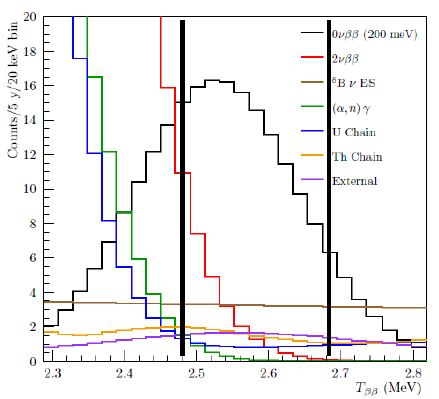
\includegraphics[angle=0,width=0.75\textwidth]{plots/SNOp_backgrounds.JPG}
\caption{SNO+ Phase I signal and background energy spectrum (visible kinetic energy reconstructed under a $\vbb$ hypothesis). Plot taken from~\cite{SNOp_paper}}
\label{fig:SNOp_bkgs}
\end{figure}

The event topology of $\vbb$- and $\vvbb$-decays are very similar - both produce two electron tracks in the detector. As shown in Fig.~\ref{fig:Kinematics}, in the region of interest (ROI) where total kinetic energy of the electrons is close to the energy spectrum end point (Q-value), there is almost no difference in kinematic distributions between $\vbb$- and $\vvbb$-decays. Therefore the energy resolution is the key parameter for discrimination between these two processes in any detector searching for $\vbb$-decay.

\begin{figure}[htb]
\centering
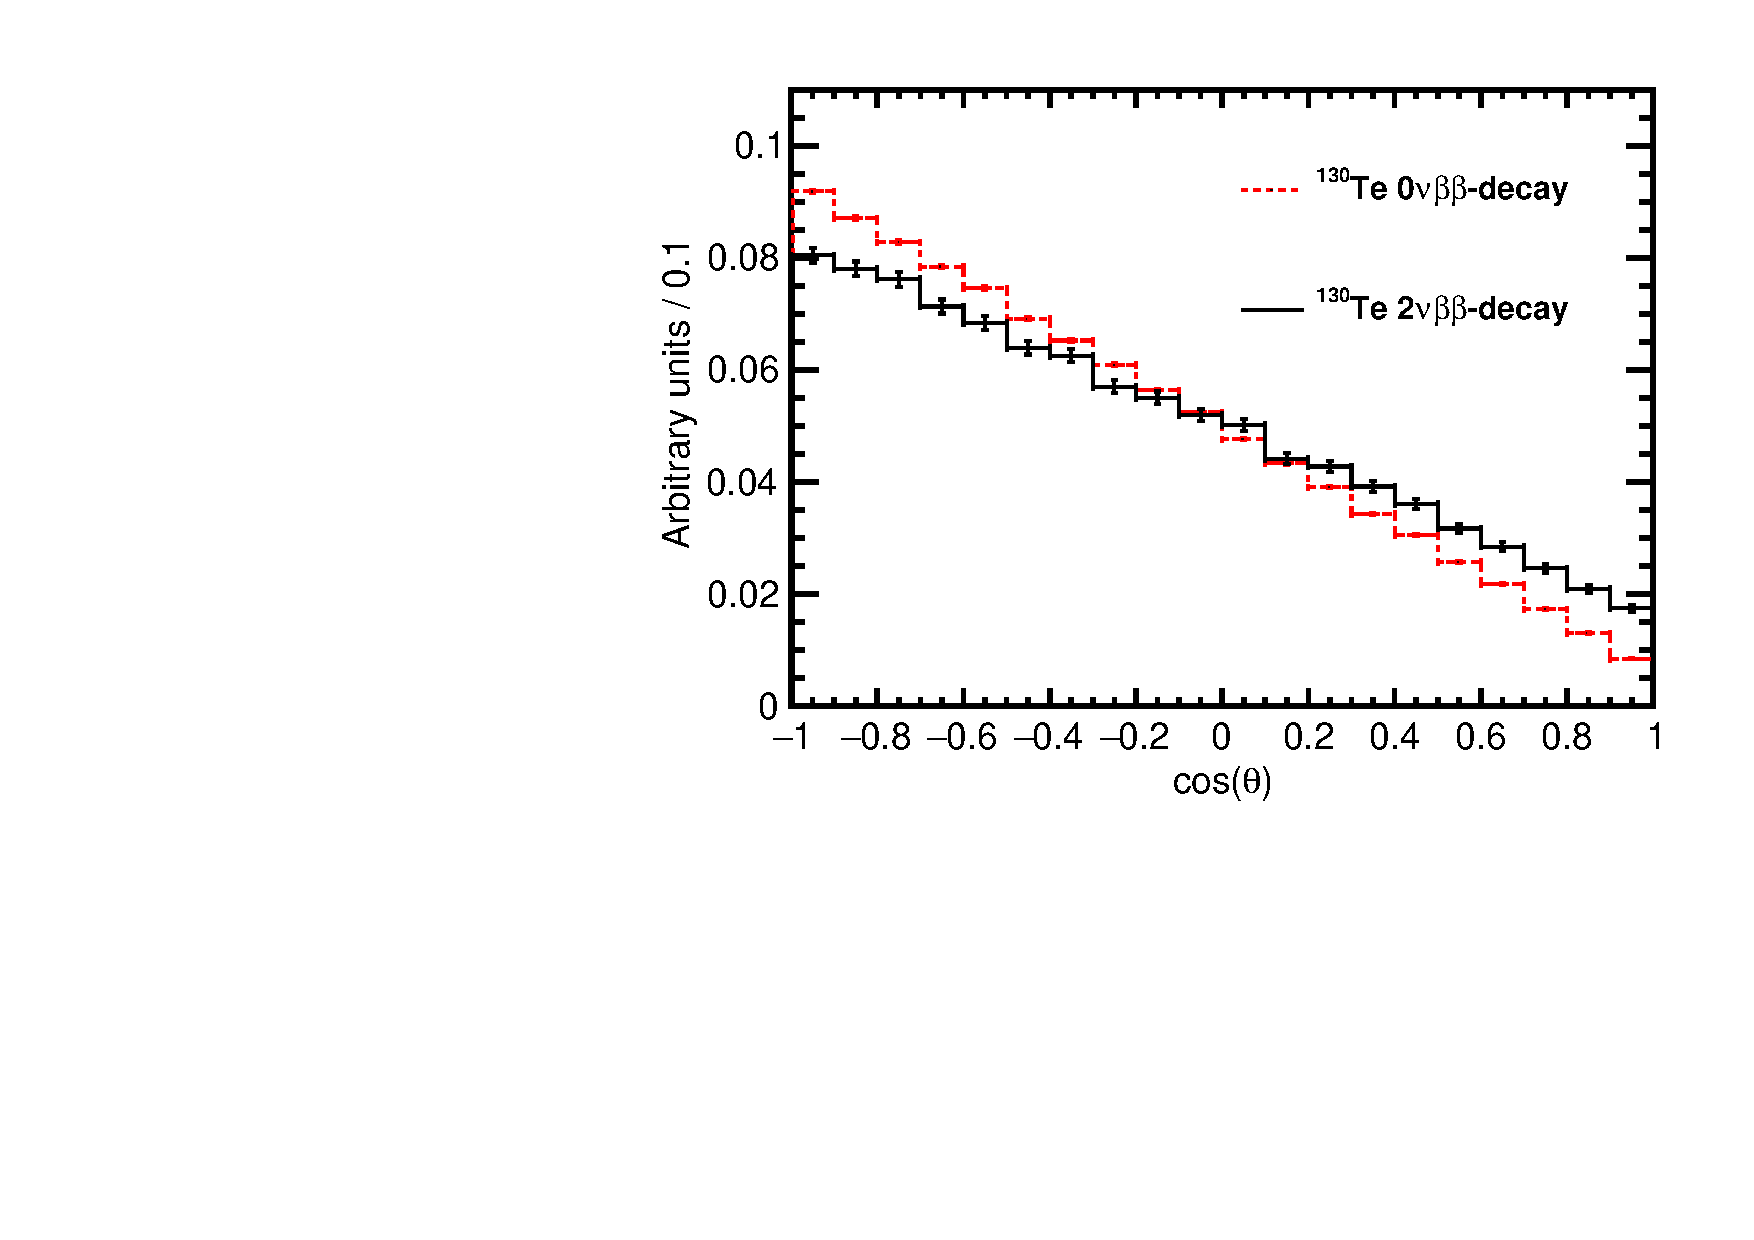
\includegraphics[angle=0,width=0.49\textwidth]{plots/hCos_Te130.pdf}
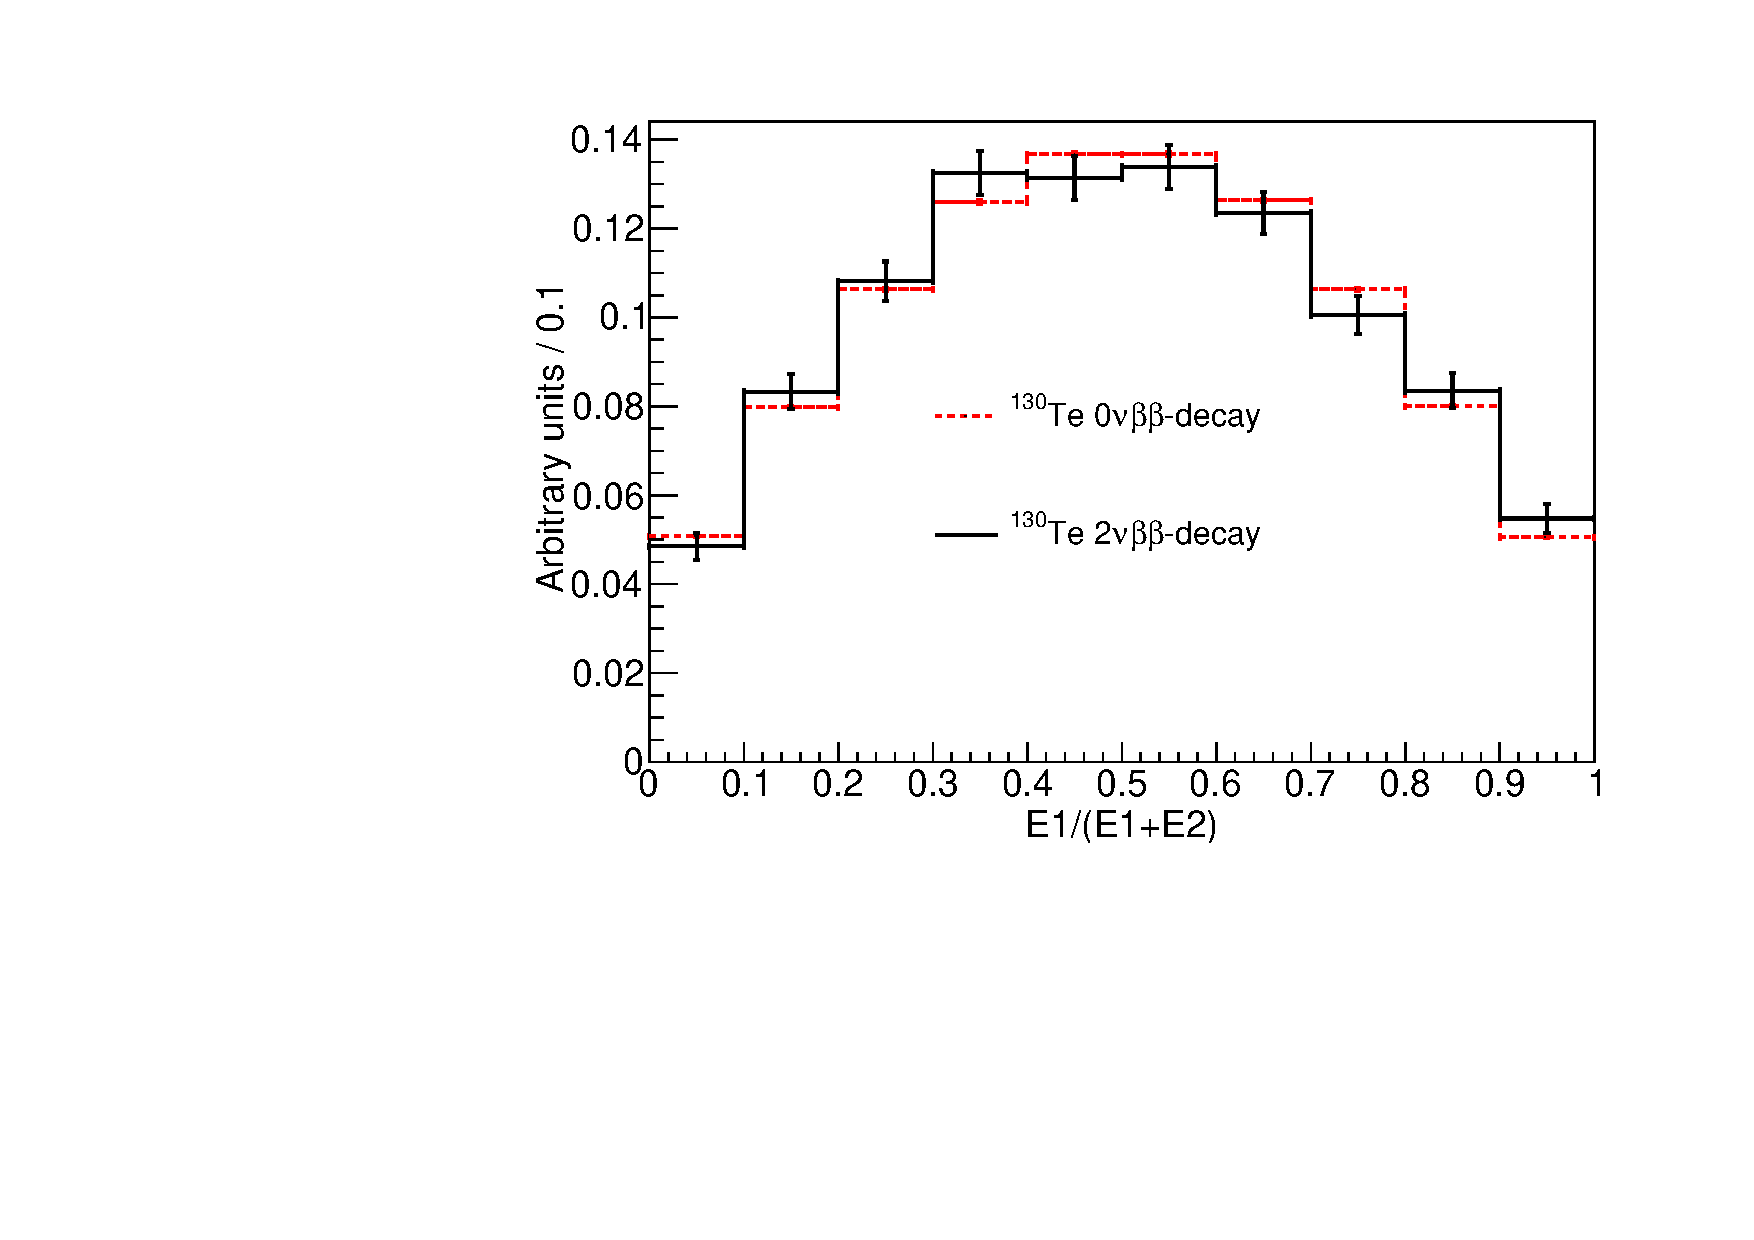
\includegraphics[angle=0,width=0.49\textwidth]{plots/hE1toQ_Te130.pdf}
\caption{Comparison between kinematics of $\vbb$- (dashed red lines) and $\vvbb$-decays (solid black lines) for events with the total kinetic energy of the electrons above 90\% of the Q-value. (Left) Cosine of the angle between two electrons. (Right) Fraction of energy carried by one of the two electrons. Due to limited statistic around the energy spectrum end point for $\vvbb$-decay we show statistical errors for each bin.}
\label{fig:Kinematics}
\end{figure}


While the event topology of $\vvbb$-decay is very similar to the $\vbb$-decay, the topology of the next largest background coming from the $\B$ solar neutrino is sufficiently different and can be used to suppress this type of background. 

$\B$ solar neutrino interactions produce only one electron. In a liquid scintillator detector the difference between two electrons and one electron will show up in the distribution of the Cherenkov photons. Abundant scintillation light makes it challenging to extract small Cherenkov light contribution from low energy electrons. However, as have been shown in our previous work, photo-detectors with time resolution of $\sim$100~ps can allow for selection of photons that contain significant fraction of Cherenkov light produced by 1-5~MeV electrons in a kilo-ton scale liquid scintillator detector. Cherenkov photons on average arrive to the detector surface earlier than scintillation light due to longer wavelength of the Cherenkov photons and a delay in the scintillation process. Thus early light primarily consist of Cherenkov photons.

In this paper we propose to use spherical harmonics to analyze distributions of the early photo-electrons (PE) for discrimination between $\B$ background and $\vbb$-decay signal.

Section~\ref{sec:detector_description} describes our detector model. Section~\ref{sec:topology_and_harmonics} introduces spherical harmonics analysis. Performance and experimental challenges are discussed in Sec.~\ref{sec:performance_and_challenges}


\section{Detector Model}
\label{sec:detector_description}
{\bf Copy info from~\cite{Directionality}.

Figures~\ref{fig:Arrival_time} and~\ref{fig:NPhot} show simulation output relevant for further discussion.}

\begin{figure}[htb]
\centering
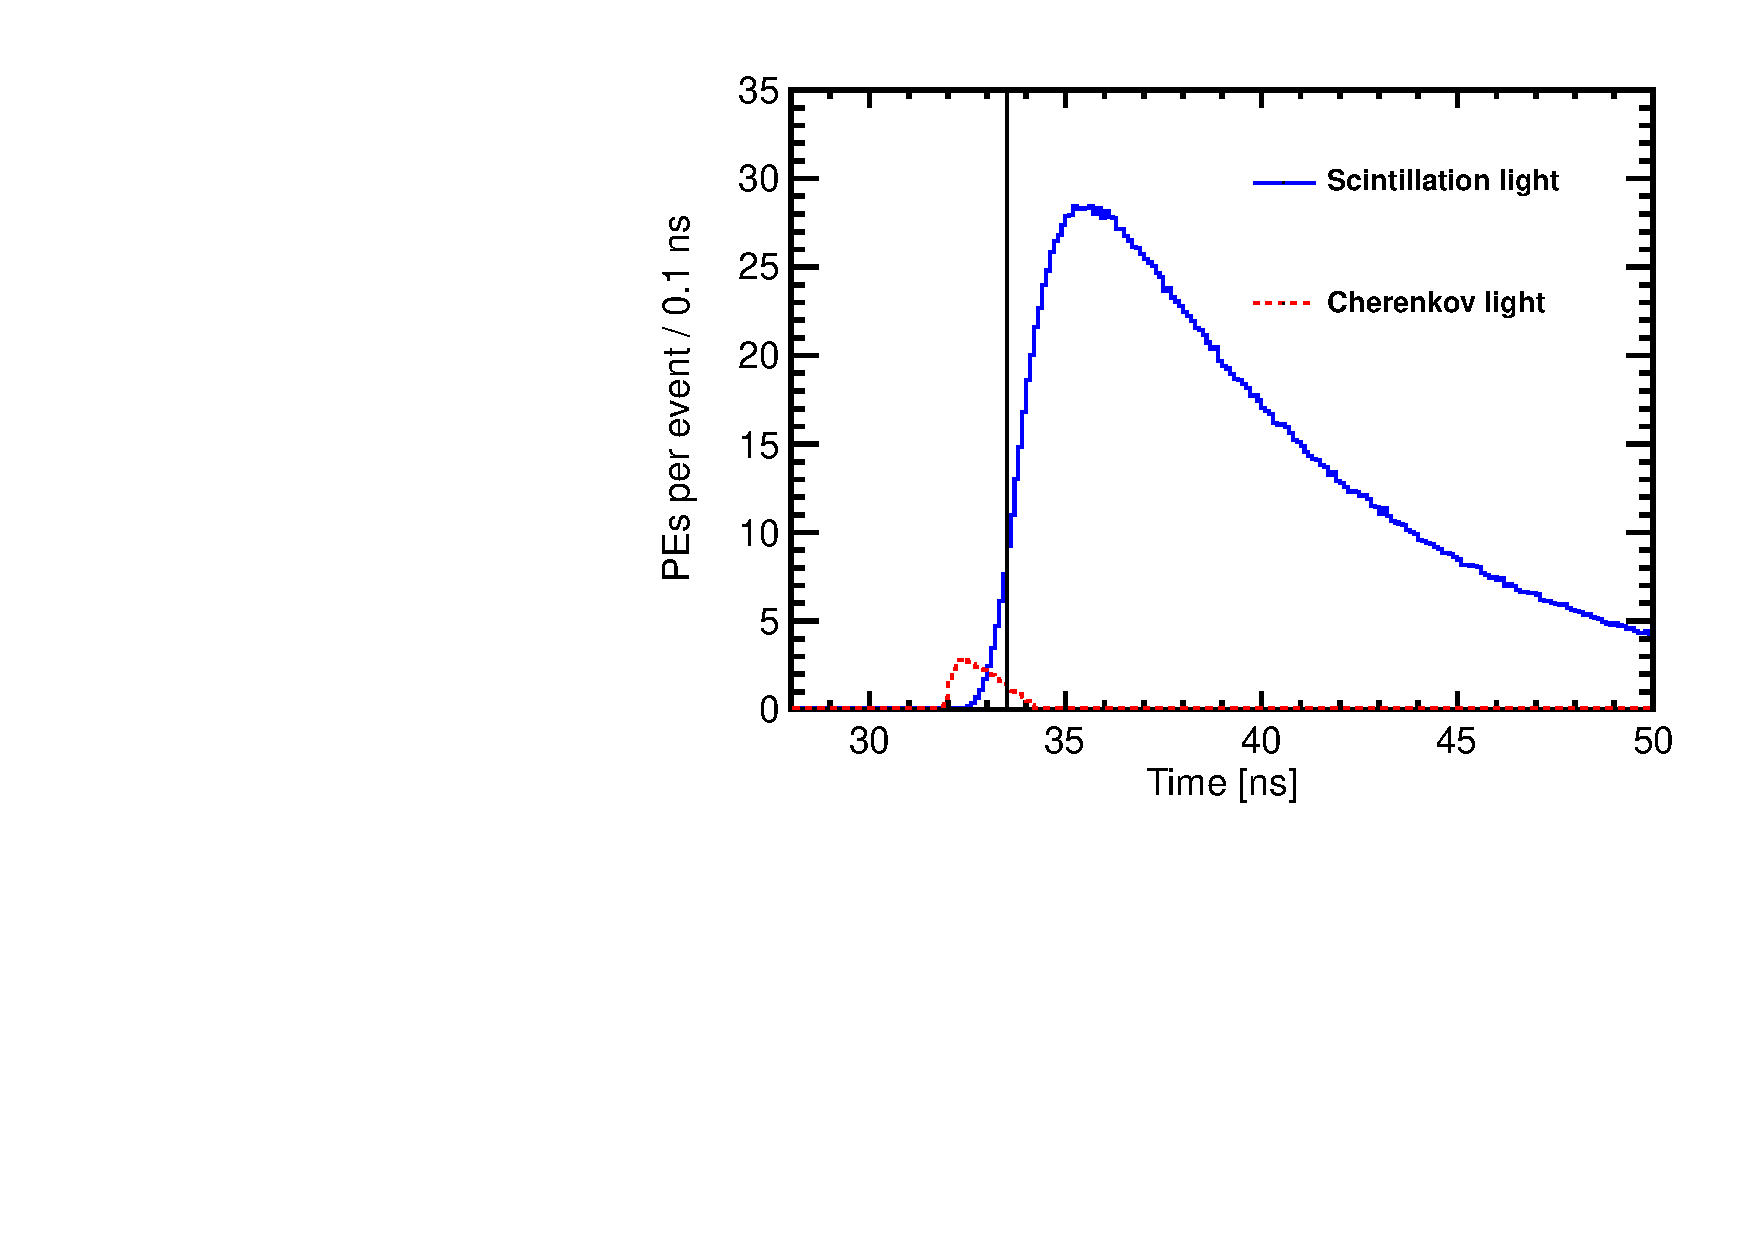
\includegraphics[angle=0,width=0.45\textwidth]{plots/hT_Te130.pdf}
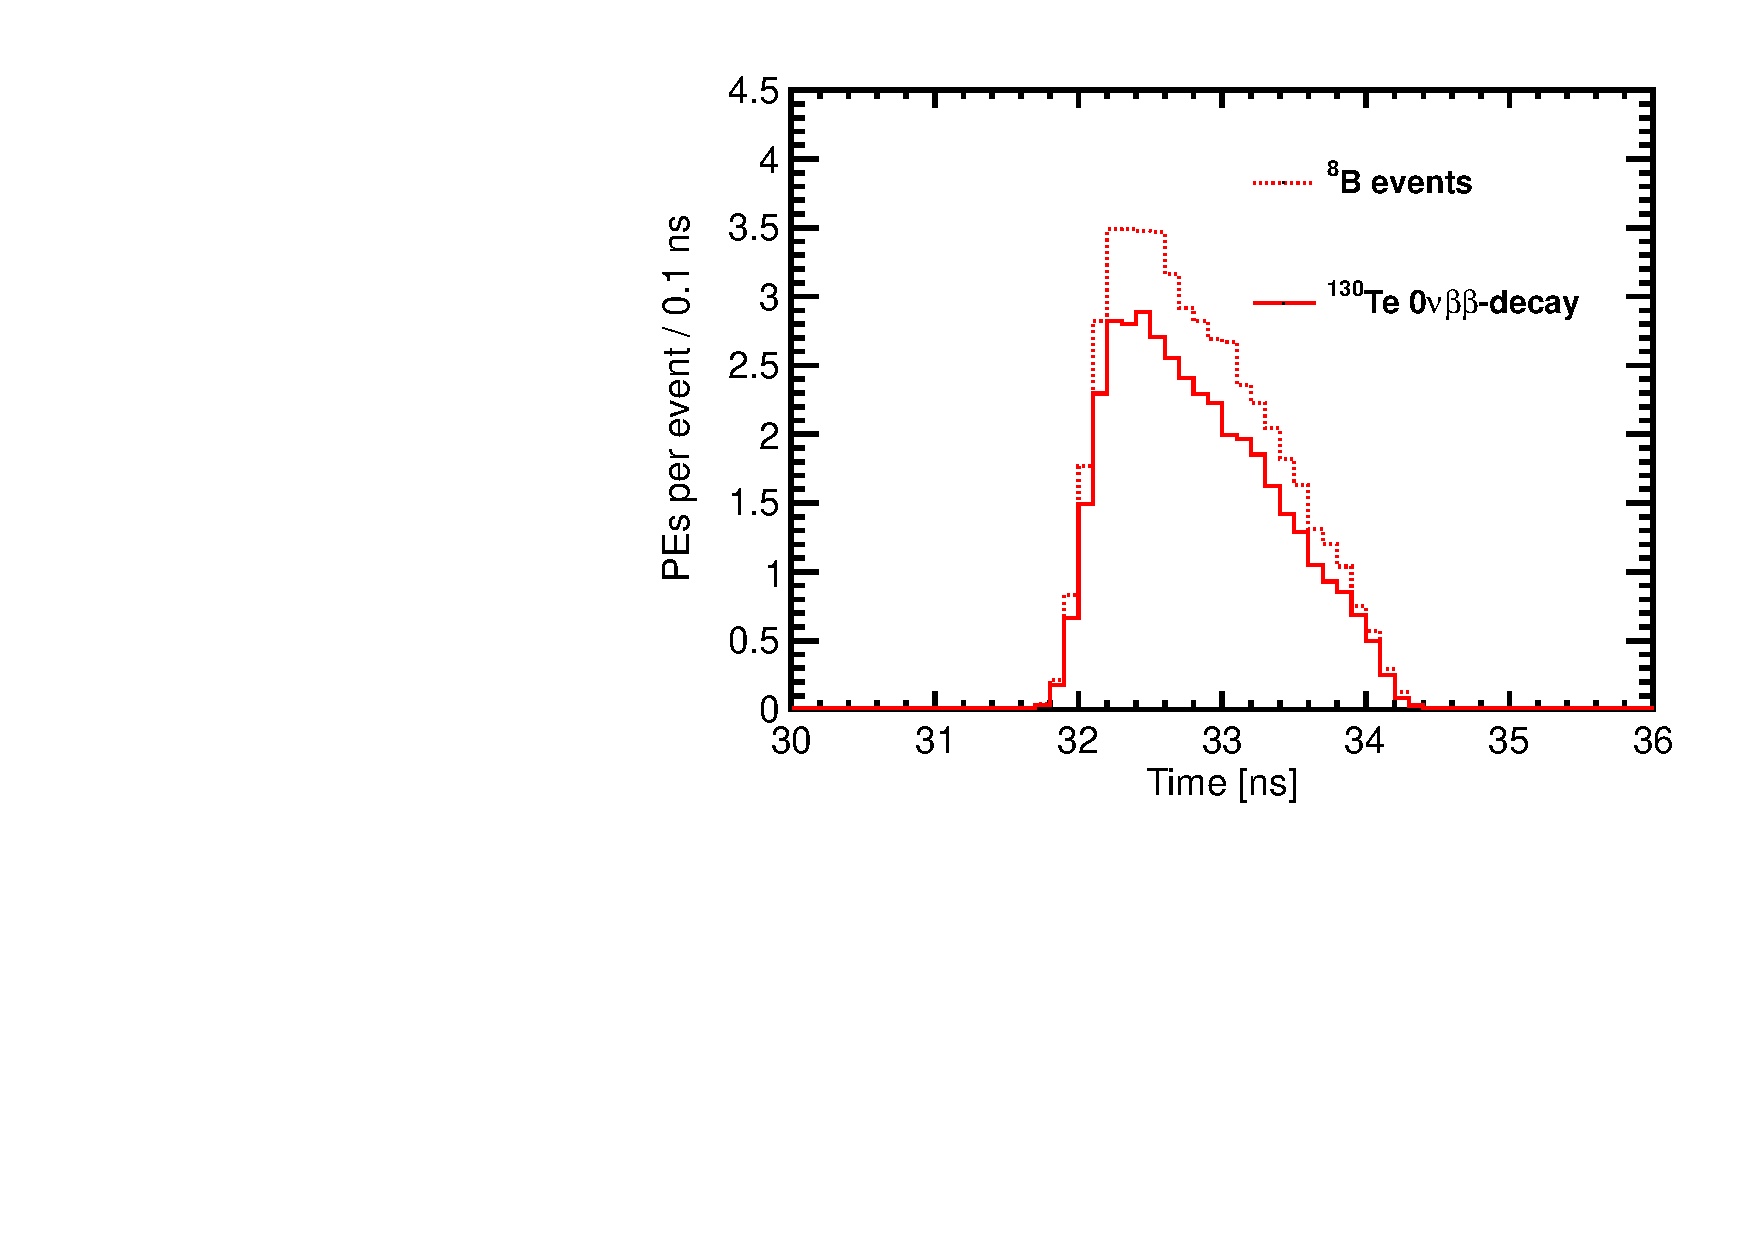
\includegraphics[angle=0,width=0.45\textwidth]{plots/hTche_Te130_B8.pdf}
\caption{(Left) Photo-electron (PE) arrival times after application of the photo-detector transit time spread (TTS) of 100~ps for the simulation of 1000 $\vbb$-decay events of $\Te$ at the center of the detector. PEs from Cherenkov light (red, dash line) and scintillation light (blue, solid
line) are compared. The black vertical line illustrates a time cut at 33.5 ns. (Right) Comparison between Cherenkov PEs arrival time for $\Te$ $\vbb$-decay (solid line) and $\B$ (dotted line) events. {\bf Distributions of the scintillation PEs arrival time are indistinguishable between $\Te$ $\vbb$-decay and $\B$ due to identical total energy in the event, Q($\Te$)$=$2.529~MeV.} }
\label{fig:Arrival_time}
\end{figure}


\begin{figure}[htb]
\centering
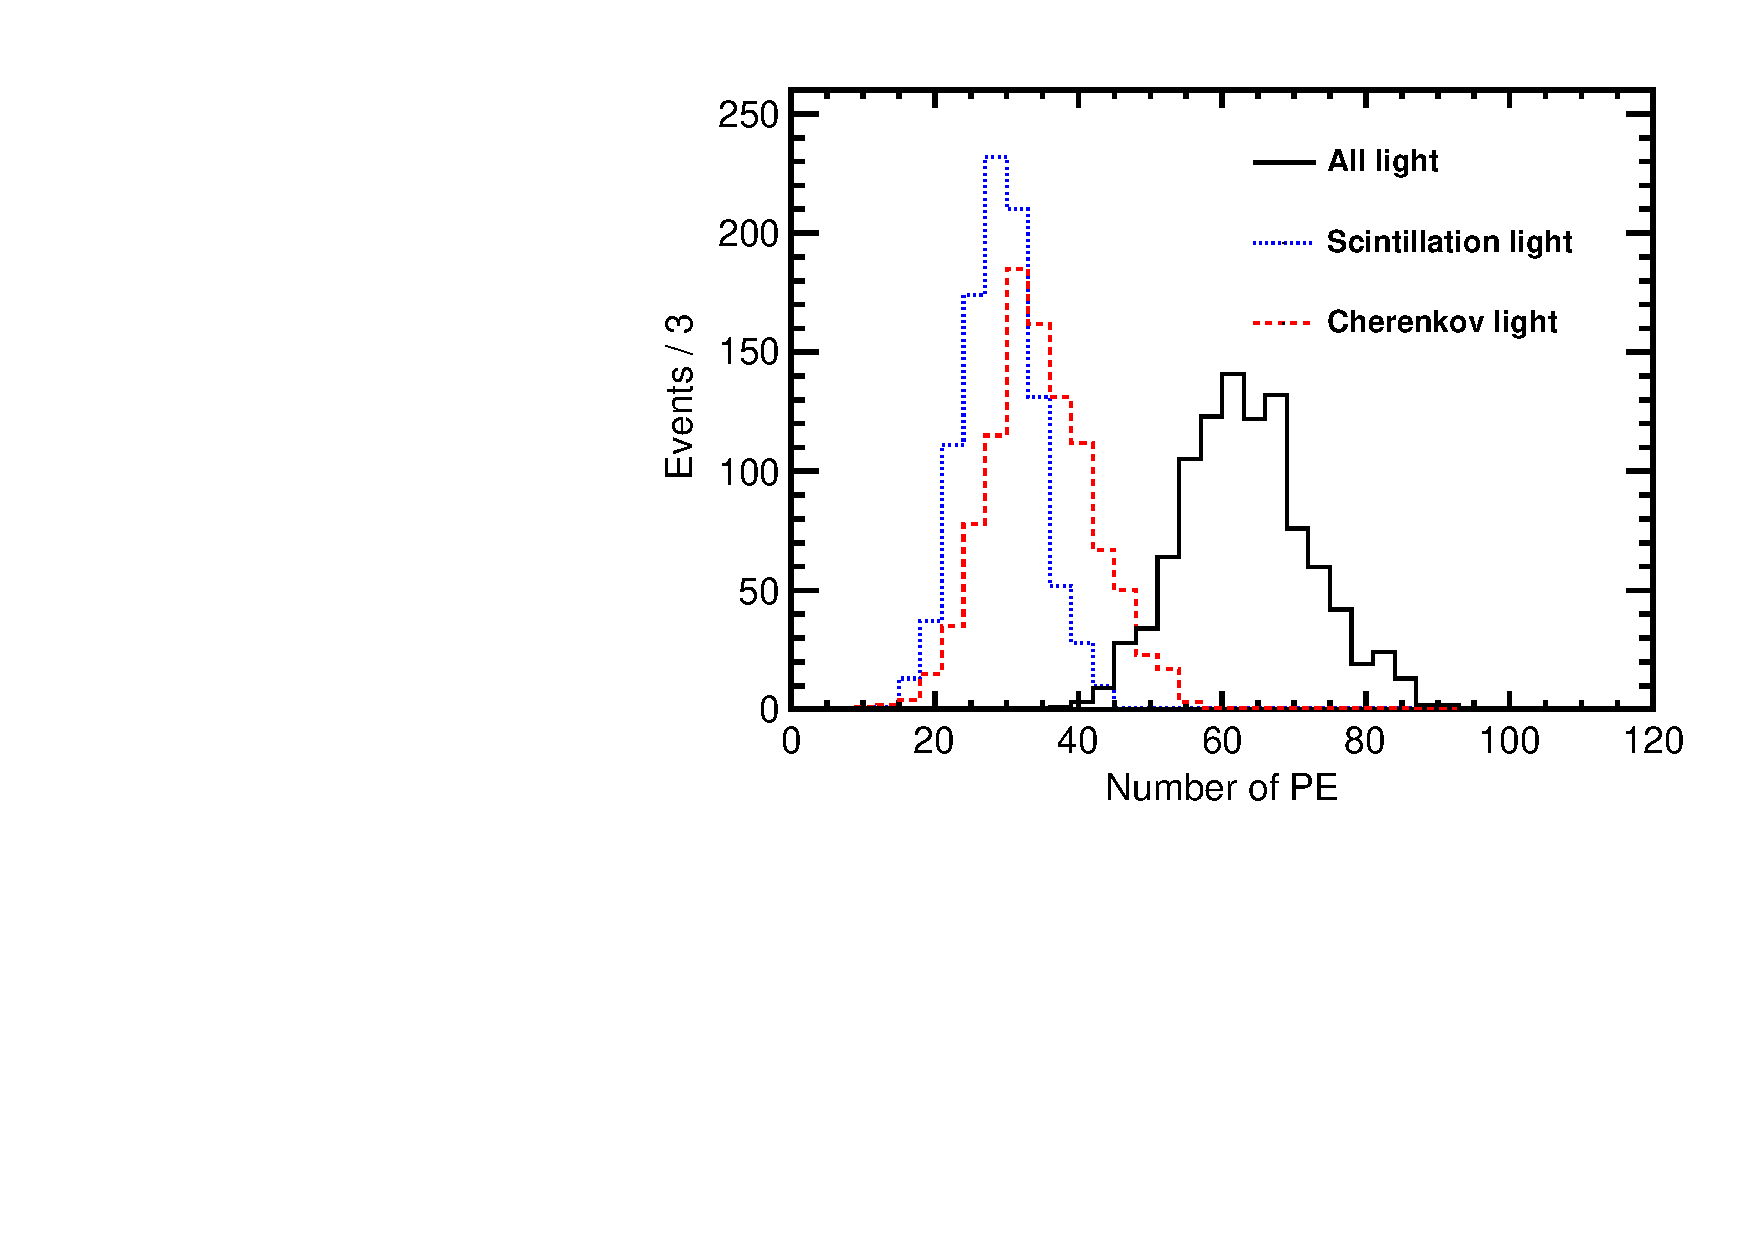
\includegraphics[angle=0,width=0.45\textwidth]{plots/hMomNPhot_Te130.pdf}
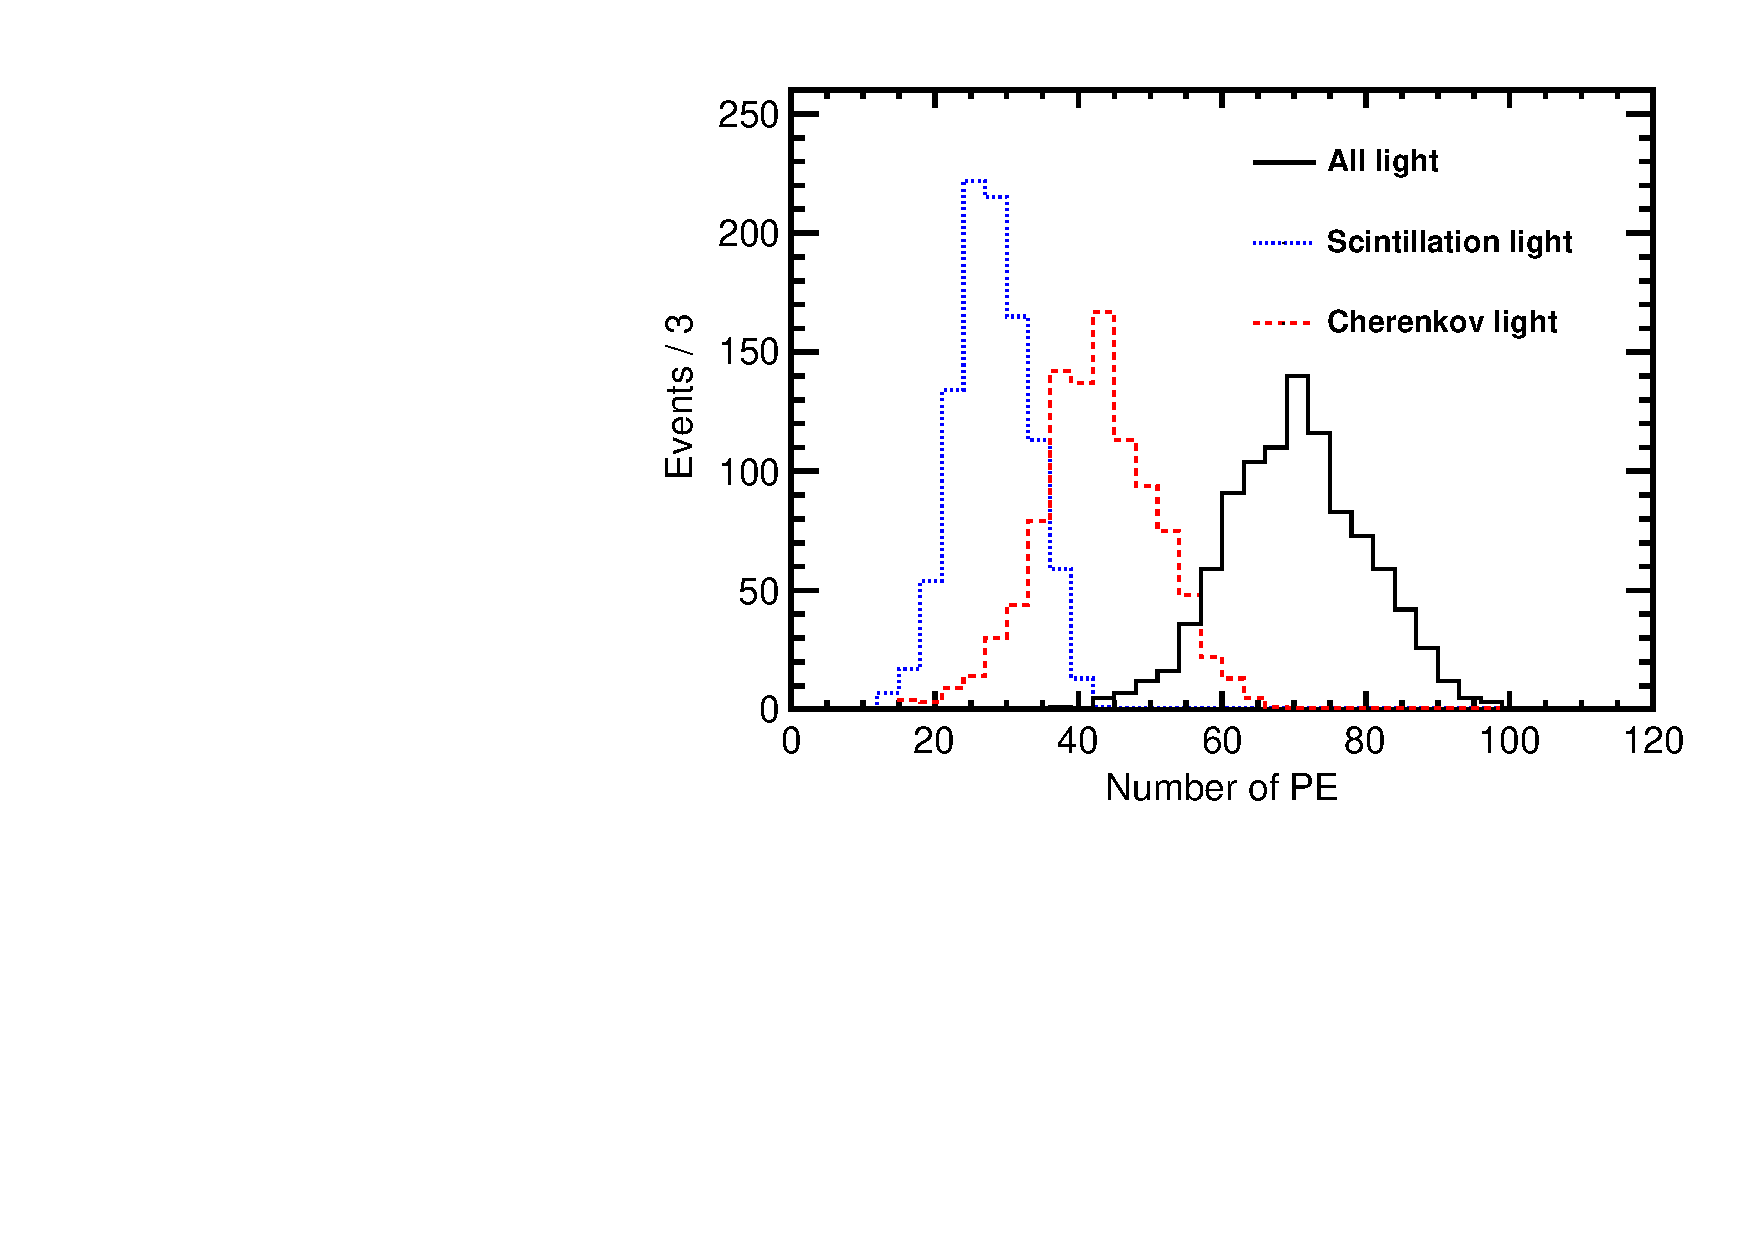
\includegraphics[angle=0,width=0.45\textwidth]{plots/hMomNPhot_1el_2p529MeV.pdf}
\caption{Number of Cherenkov (red dash line), scintillation (blue dotted line), and total (black solid line) PEs for the simulatio of 1000 $\Te$ $\vbb$-decay (left panel) and $\B$ (right panel) events.}
\label{fig:NPhot}
\end{figure}


\section{Event Topology and Spherical Harmonics Analysis}
\label{sec:topology_and_harmonics}

\subsection{Topology of $\vbb$-decay and $\B$ Events}
\label{subsec:topology}
%Signature of the $\vbb$-decay is two electrons with total kinetic energy equal to the isotope Q-value (e.g., 2.529~MeV for $\Te$). Therefore all $\vbb$-decay searches are designed to look for an excess of events in the energy spectrum around Q-value over the predicted number of background events. Backgrounds such as $\B$ solar neutrinos have distinct event topology that can be used to improve experimental sensitivity to the the $\vbb$-decay signal.

Electrons in the energy range around Q-value of all isotopes considered for $\vbb$-decay searches are above Cherenkov threshold in liquid scintillators. Each electron above the threshold will produce a fuzzy ring of Cherenkov light at the detector surface. The fuzziness of the ring depends on electron scattering. In most cases Cherenkov rings from low energy electrons degrade to randomly shaped clusters of Cherenkov photons around direction of the electron track. 

Large fraction of $\vbb$-decay events will have two Cherenkov clusters~\footnote{Only one Cherenkov cluster is produced when either the angle between the two $\vbb$-decay electrons is too small or when the energy splits between the electrons in such a way that one electron falls below the Cherenkov threshold.} as opposed to one cluster from $\B$ events. Therefore separation of $\vbb$-decay signal from $\B$ background depends on ability to identify topology of the Cherenkov light on the detector sphere on top of uniformly distributed scintillation light. We show that analysis of spherical harmonics of the early photons allows to achieve noticeable separation between $\vbb$-decay and $\B$ events.



%The simplest case for spherical harmonics analysis are events with the vertex located exactly in the center of the detector. For such event Cherenkov and scintillation light can be separated by applying a time cut on the photon arrival time as demonstrated in~\cite{Directionality}. To introduce the technique of spherical harmonics analysis we will follow the same strategy as in~\cite{Directionality} and use central events with a slightly different cut on the photon arrival time of 33.5~ns.

In order to illustrate differences between different event topologies we introduce three event topologies: two electrons produced back-to-back at 180$^{\circ}$ angle, two electrons at 90$^{\circ}$ angle, and a single electron. The two former are representative topologies of $\vbb$-decay signal events and the latter represents $\B$ background events. Figure~\ref{fig:Display_top_5MeV} shows Cherenkov photon distributions of 5~MeV electrons for each of the three topology. Overlay of 100 events with no QE applied is shown in order to make Cherenkov rings visible.

\begin{figure}[htb]
\centering
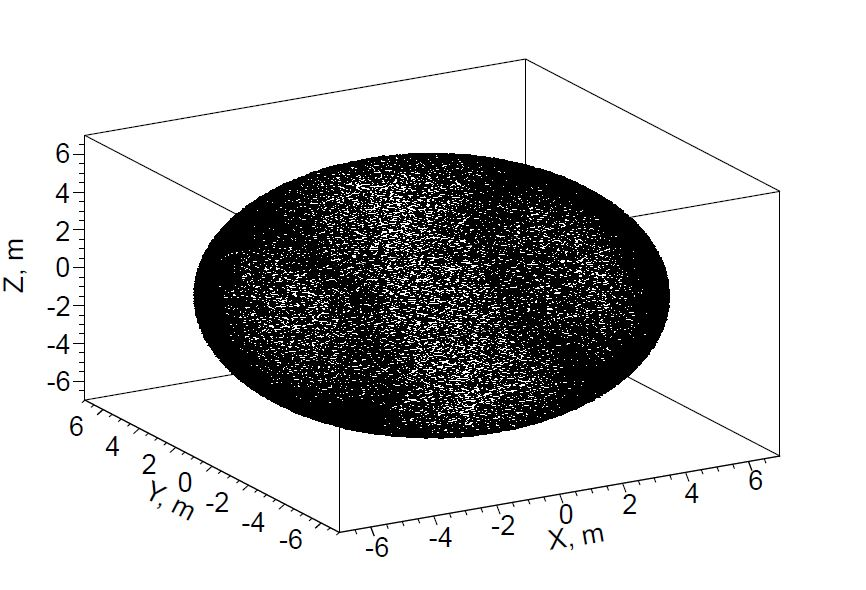
\includegraphics[angle=0,width=0.3\textwidth]{plots/hDisplay_topology180_5MeV.JPG}
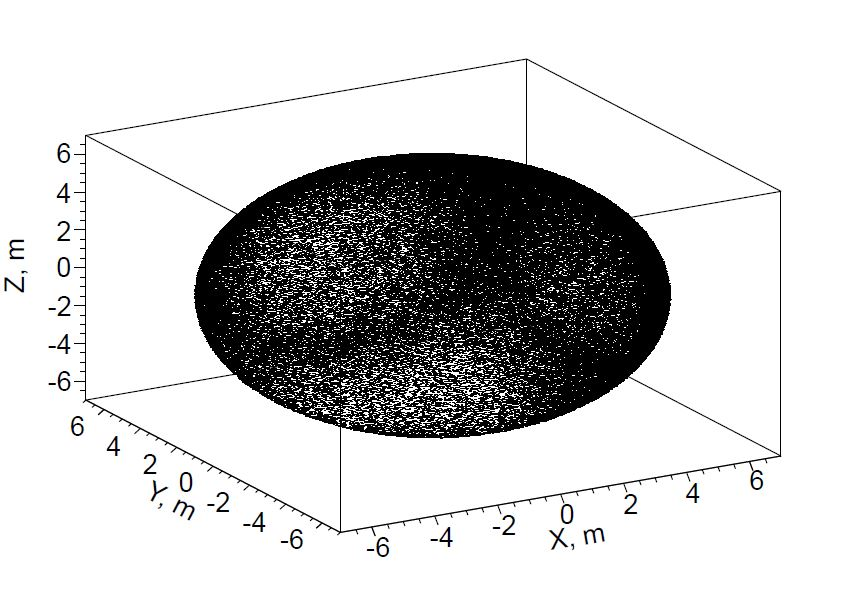
\includegraphics[angle=0,width=0.3\textwidth]{plots/hDisplay_topology90_5MeV.JPG}
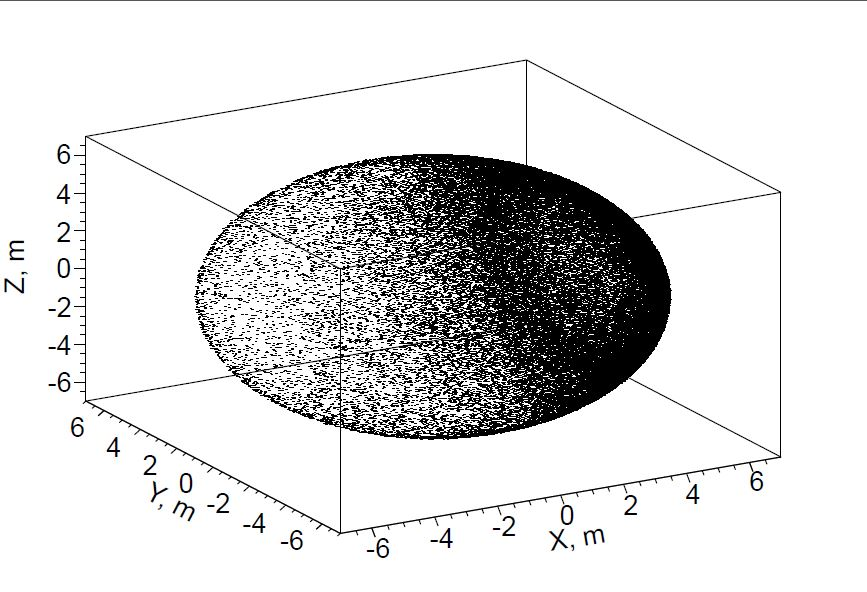
\includegraphics[angle=0,width=0.3\textwidth]{plots/hDisplay_1el_5MeV.JPG}
\caption{Cherenkov photons distributions on the detector sphere for the three representative event topologies: two back-to-back electrons (Left), two electrons at 90$^{\circ}$ angle (Middle), and a single electron (Center).  All electrons are 5~MeV and originate at the center of the detector. 100 events overlayed for better visibility of the Cherenkov rings. 100\% QE is assumed.}
\label{fig:Display_top_5MeV}
\end{figure}

Cherenkov clusters that form at lower energies are shown in Fig.~\ref{fig:Display_top_2p5MeV}. All Cherenkov photons produced in a single event are shown for the three event topologies with total kinetic energy of 2.529~MeV that corresponds to Q-value of $\Te$. One can try to guess the event topology by comparing different segments of the detector sphere.

\begin{figure}[htb]
\centering
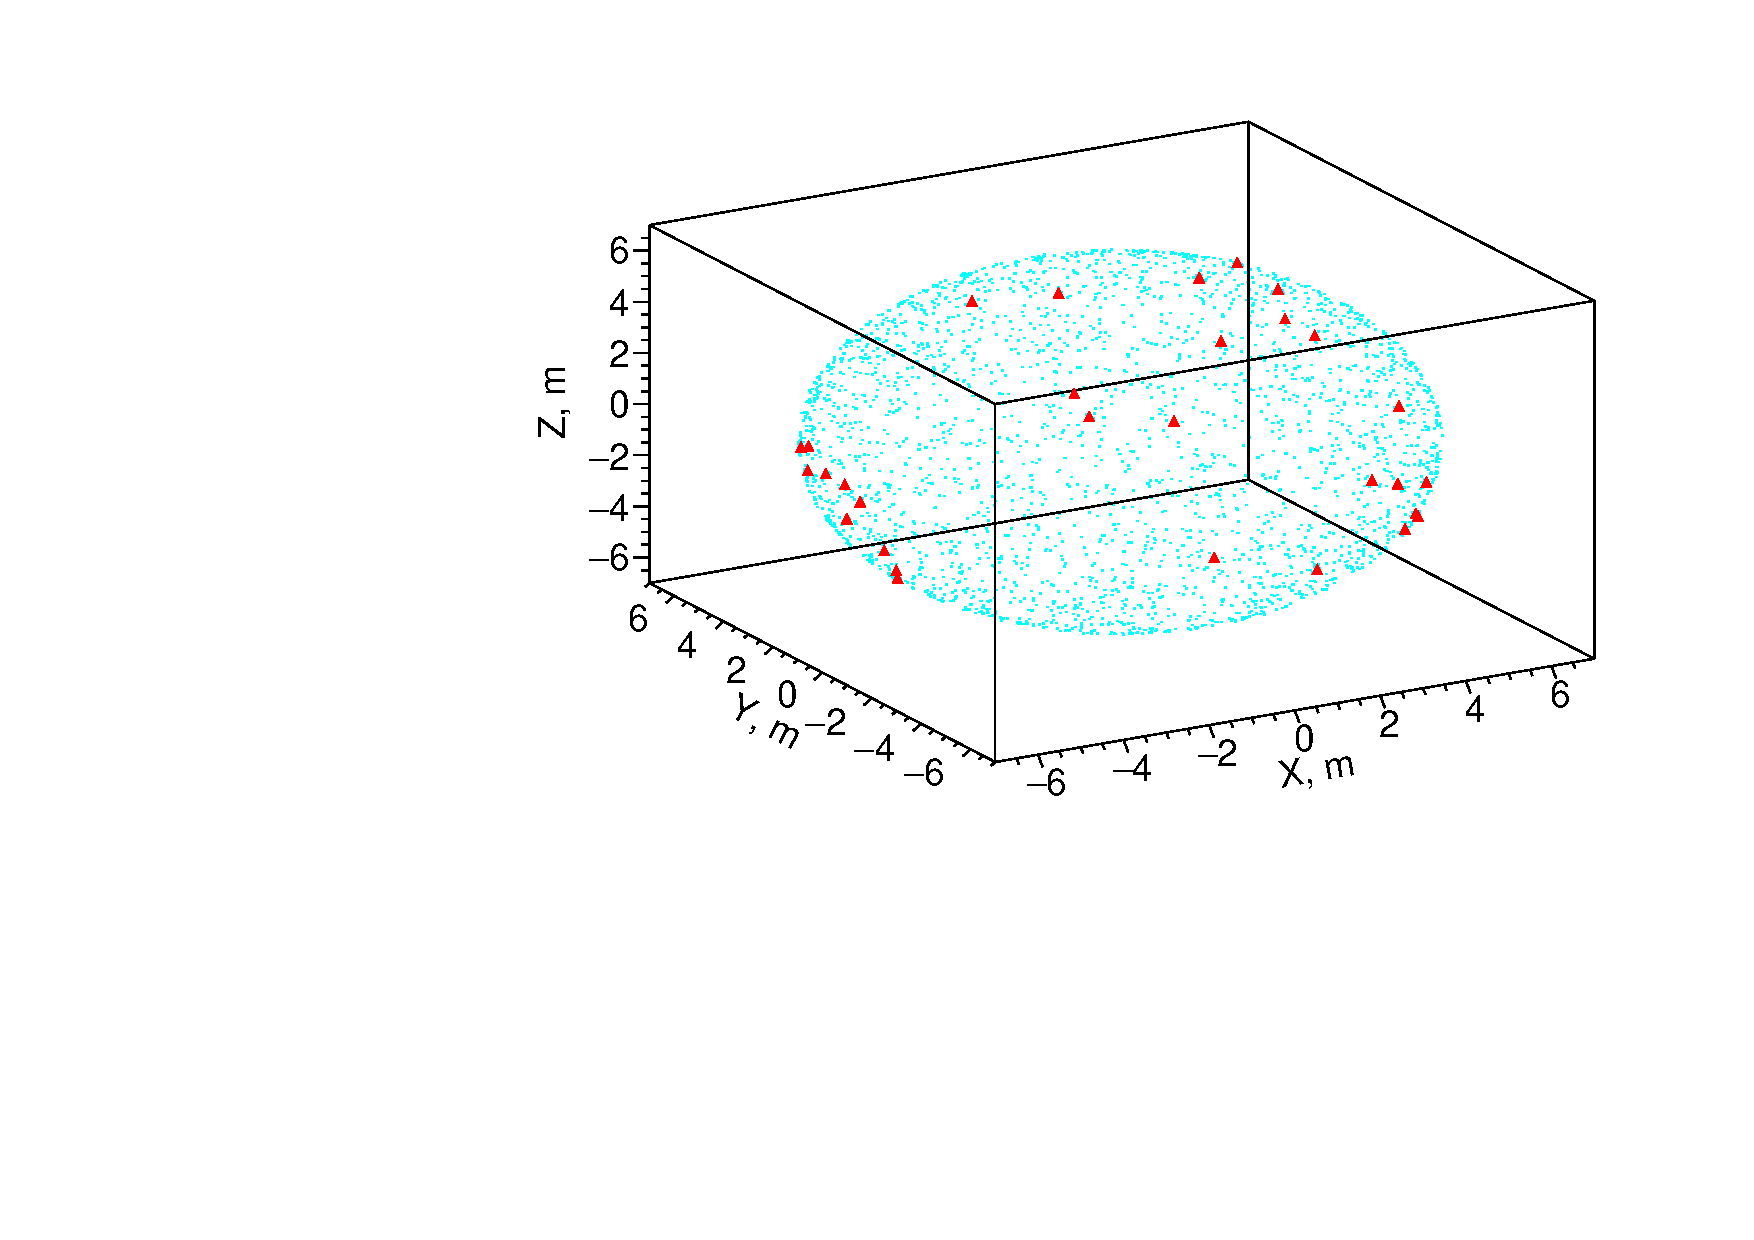
\includegraphics[angle=0,width=0.3\textwidth]{plots/hDisplay_topology180_2p529MeVTot}
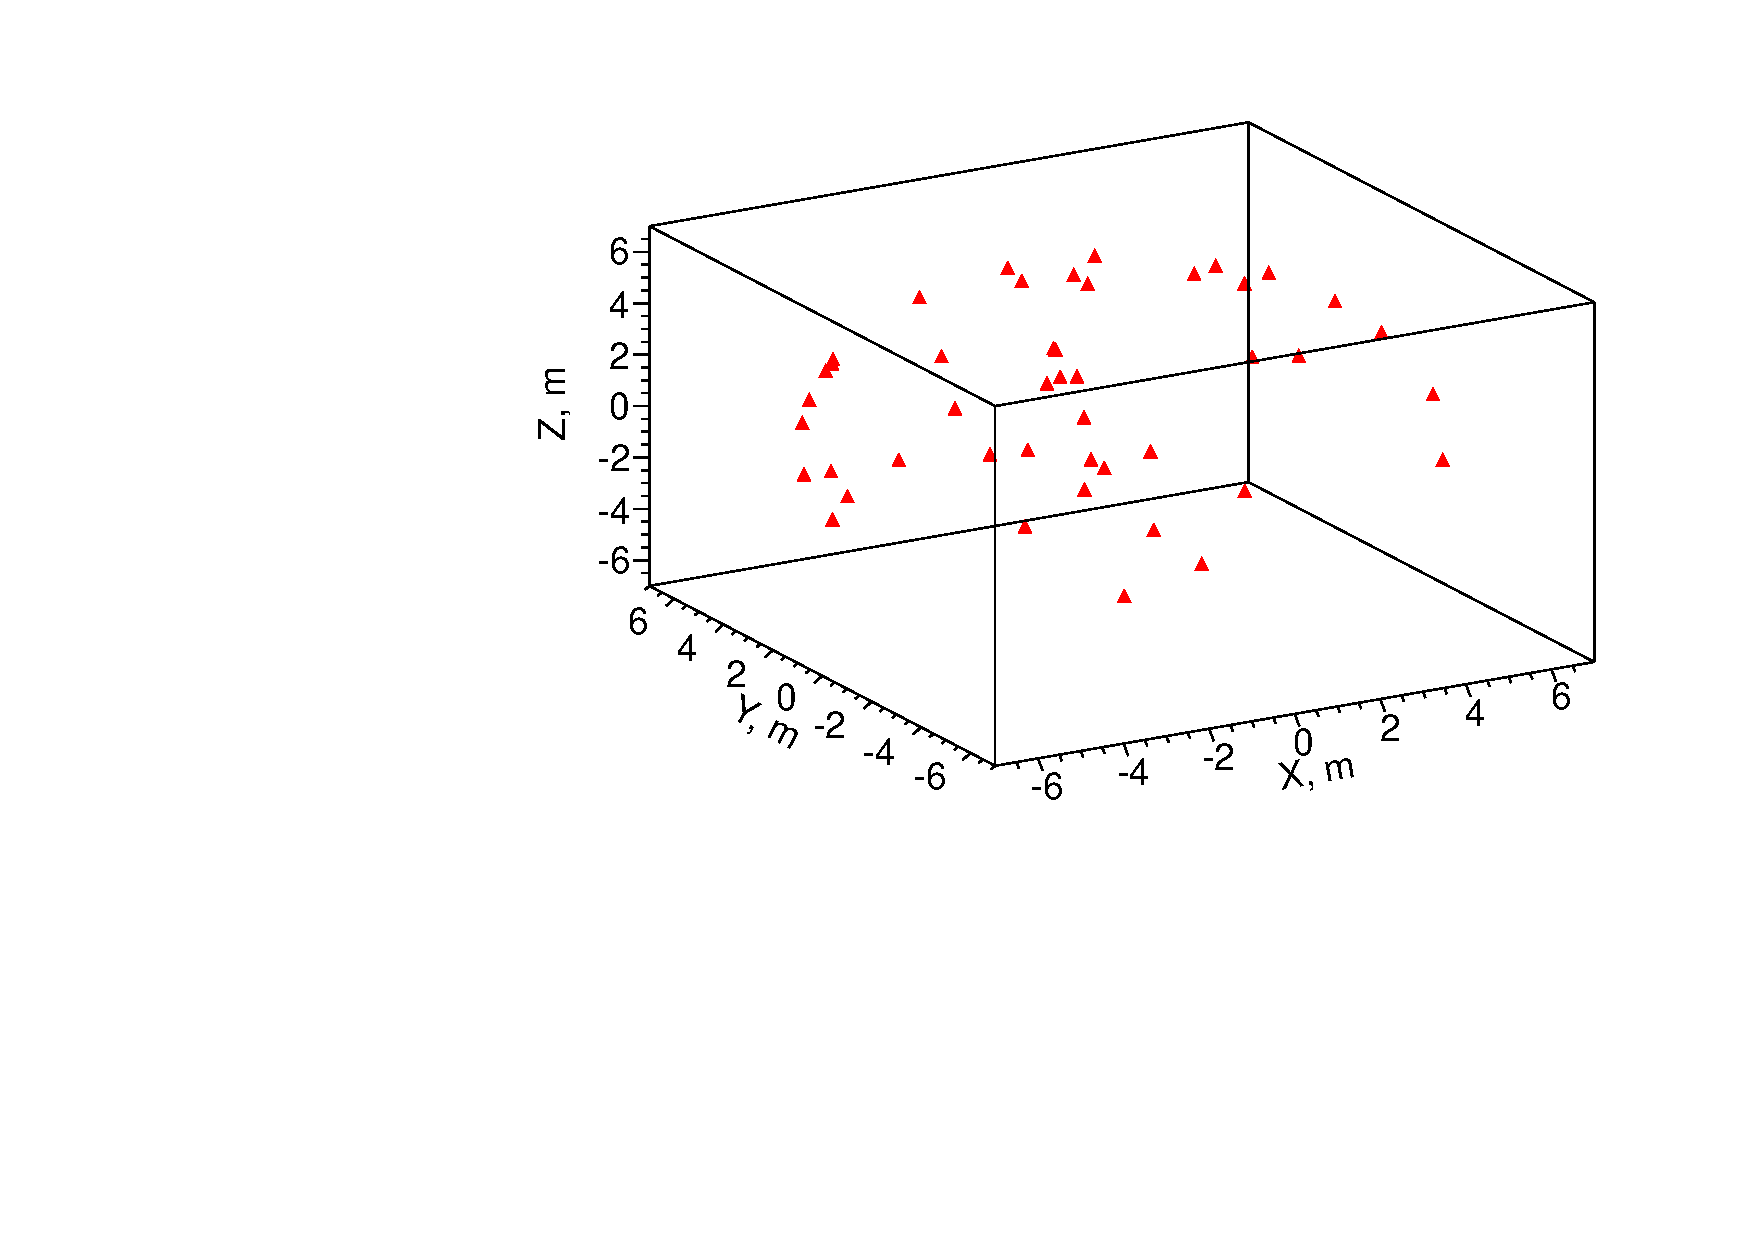
\includegraphics[angle=0,width=0.3\textwidth]{plots/hDisplay_topology90_2p529MeVTot}
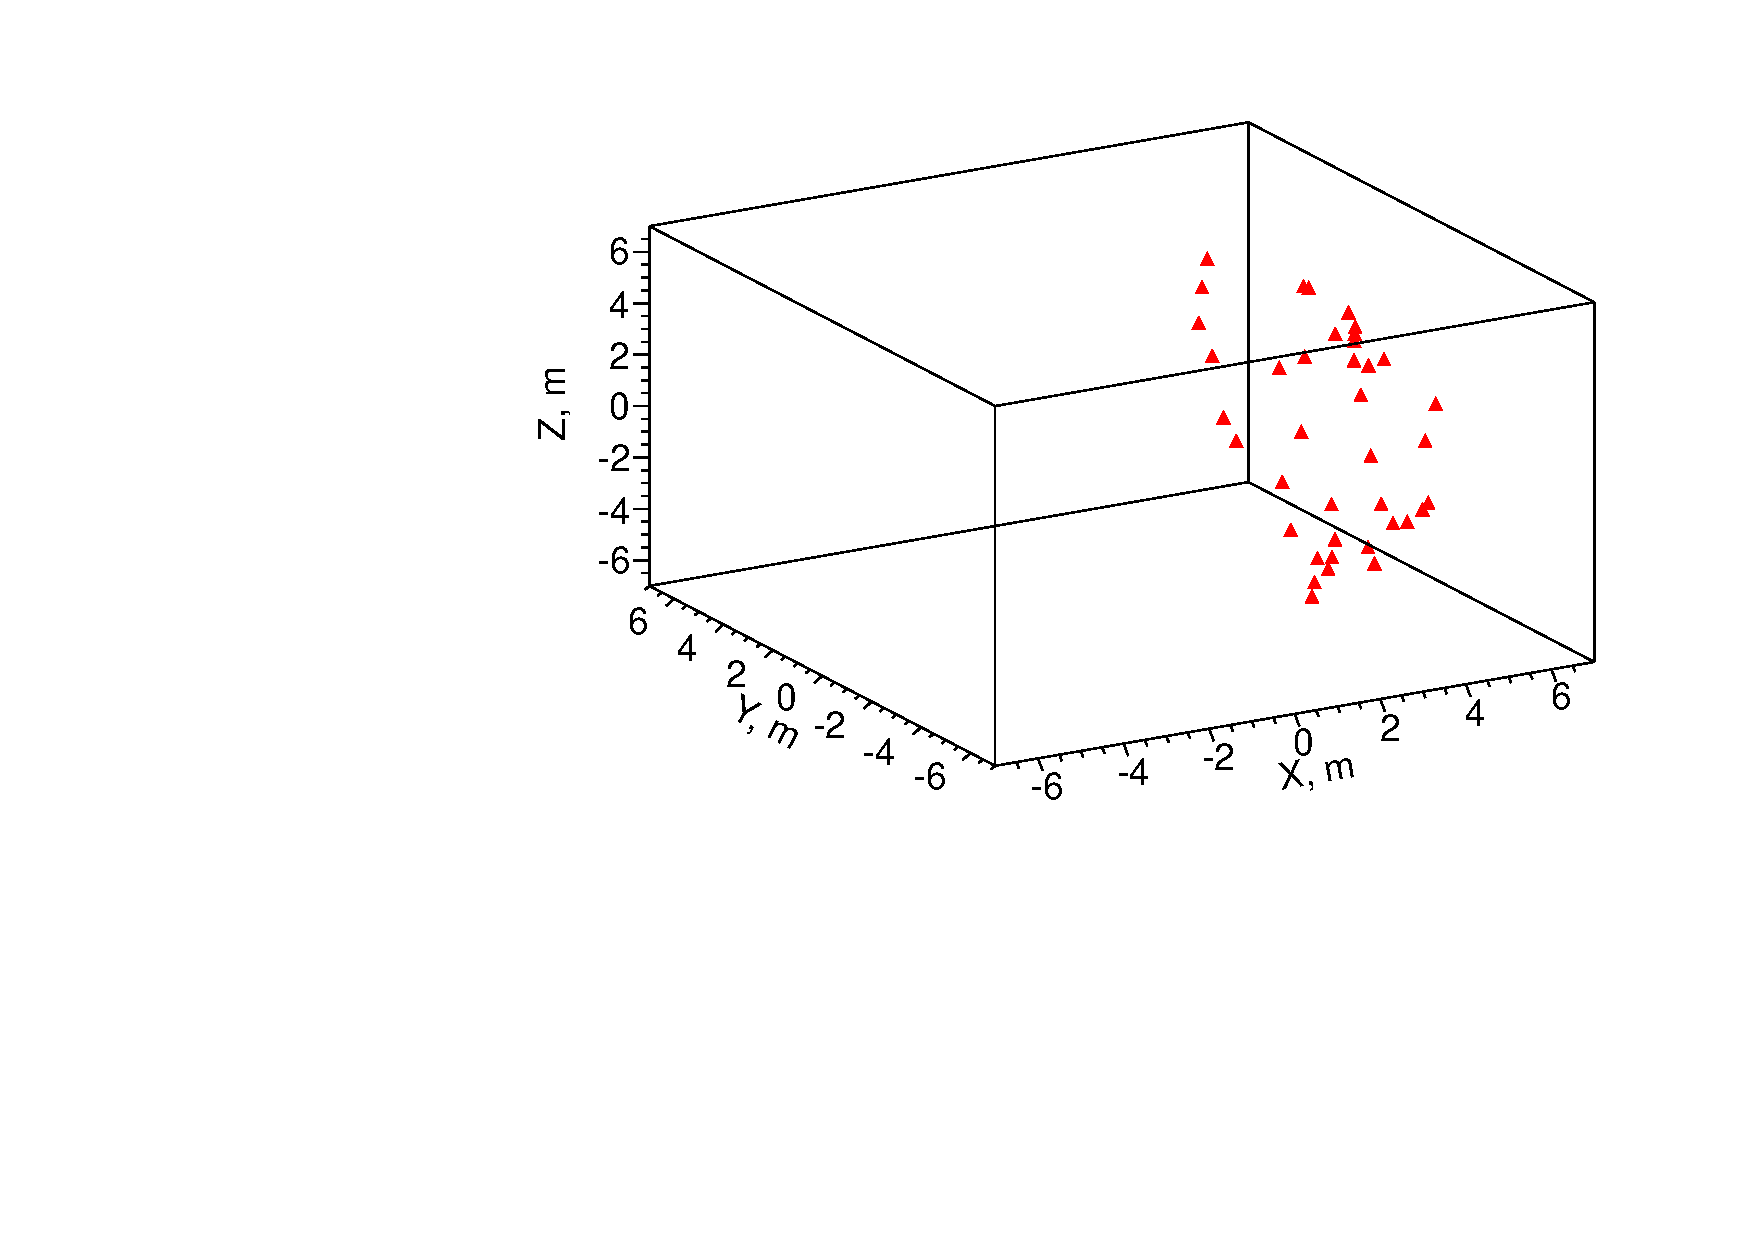
\includegraphics[angle=0,width=0.3\textwidth]{plots/hDisplay_1el_2p529MeV}
\caption{Cherenkov photons distributions on the detector sphere for the three representative event topologies: two back-to-back 1.26~MeV electrons (Left), two 1.26~MeV electrons at 90$^{\circ}$ angle (Middle), and a single 2.529~MeV electron (Center).  All electrons originate at the center of the detector. One randomly selected event is chosen for each category. Default QE is applied.}
\label{fig:Display_top_2p5MeV}
\end{figure}

More realistic examples of $\Te$ $\vbb$-decay and $\B$ events simulated at the center of the detector are shown in Fig.~\ref{fig:Display_Te130}. Early PEs from Cherenkov and scintillation light are shown. Default simulation QE is applied. Time cut of 33.5~ns on the photon arrival time is used to select early PEs. Uniformly distributed scintillation light make it more difficult to guess the event topology. Nevertheless we show that there is still sufficient difference in the spatial distribution of the early PEs to separate two track and single track events.

\begin{figure}[htb]
\centering
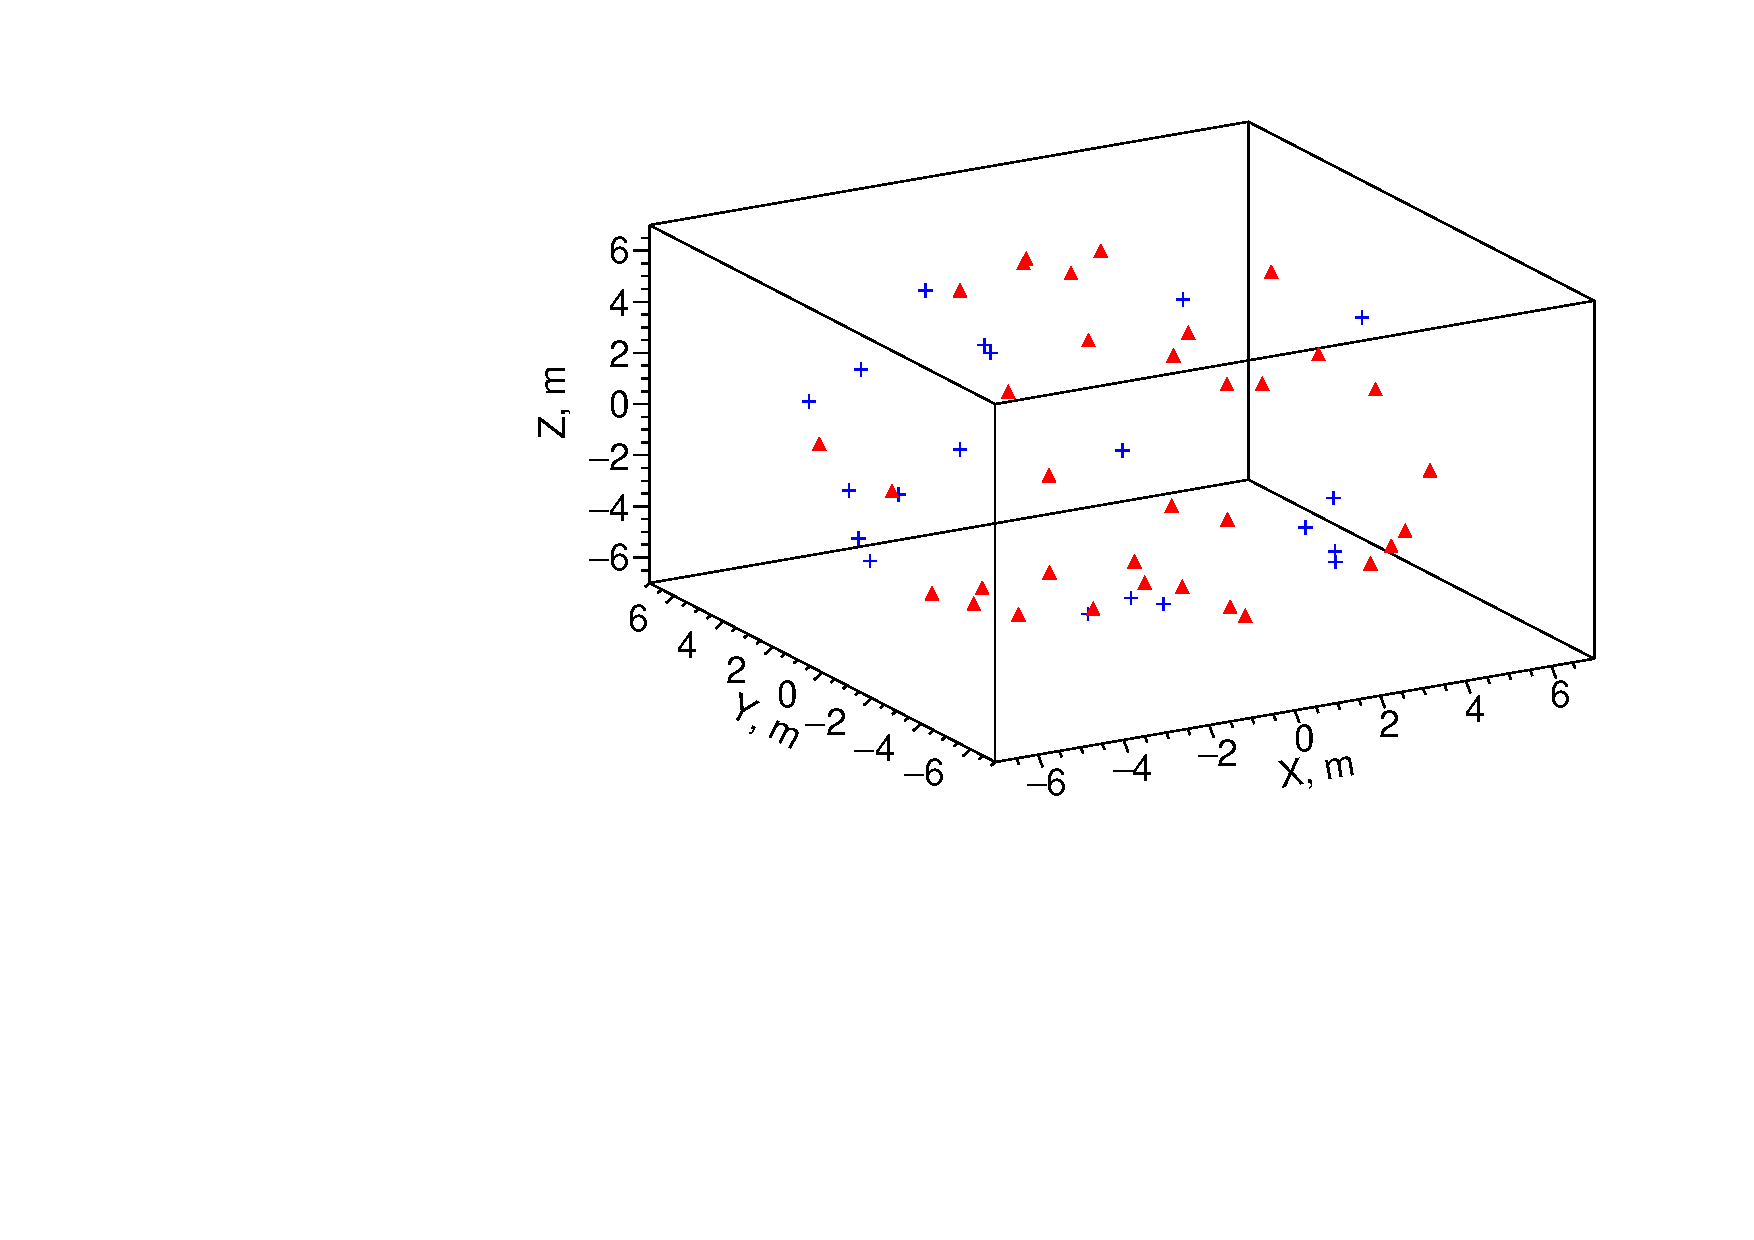
\includegraphics[angle=0,width=0.45\textwidth]{plots/hDisplay_Te130_evt124_e1257_e1270_cos-0908}
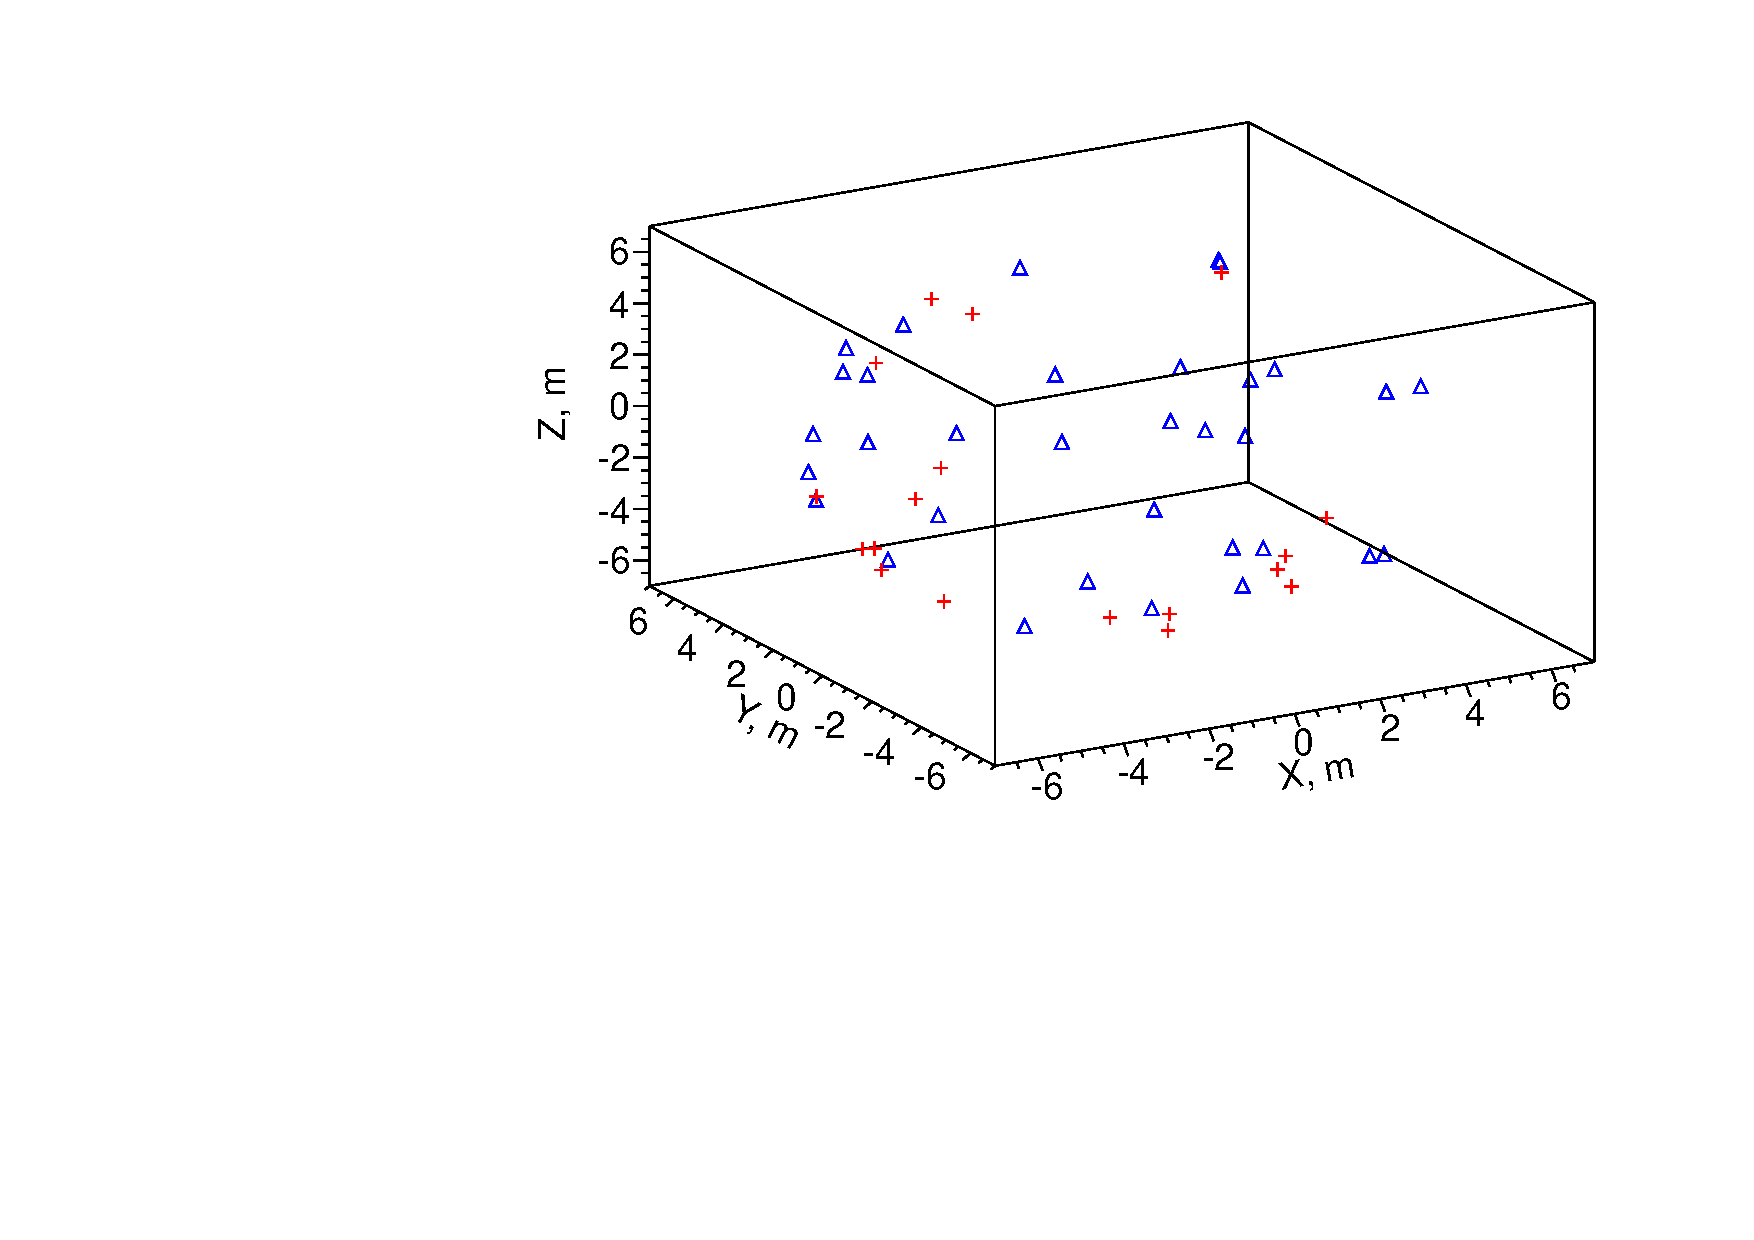
\includegraphics[angle=0,width=0.45\textwidth]{plots/hDisplay_Te130_evt131_e1264_e1263_cos-0029}
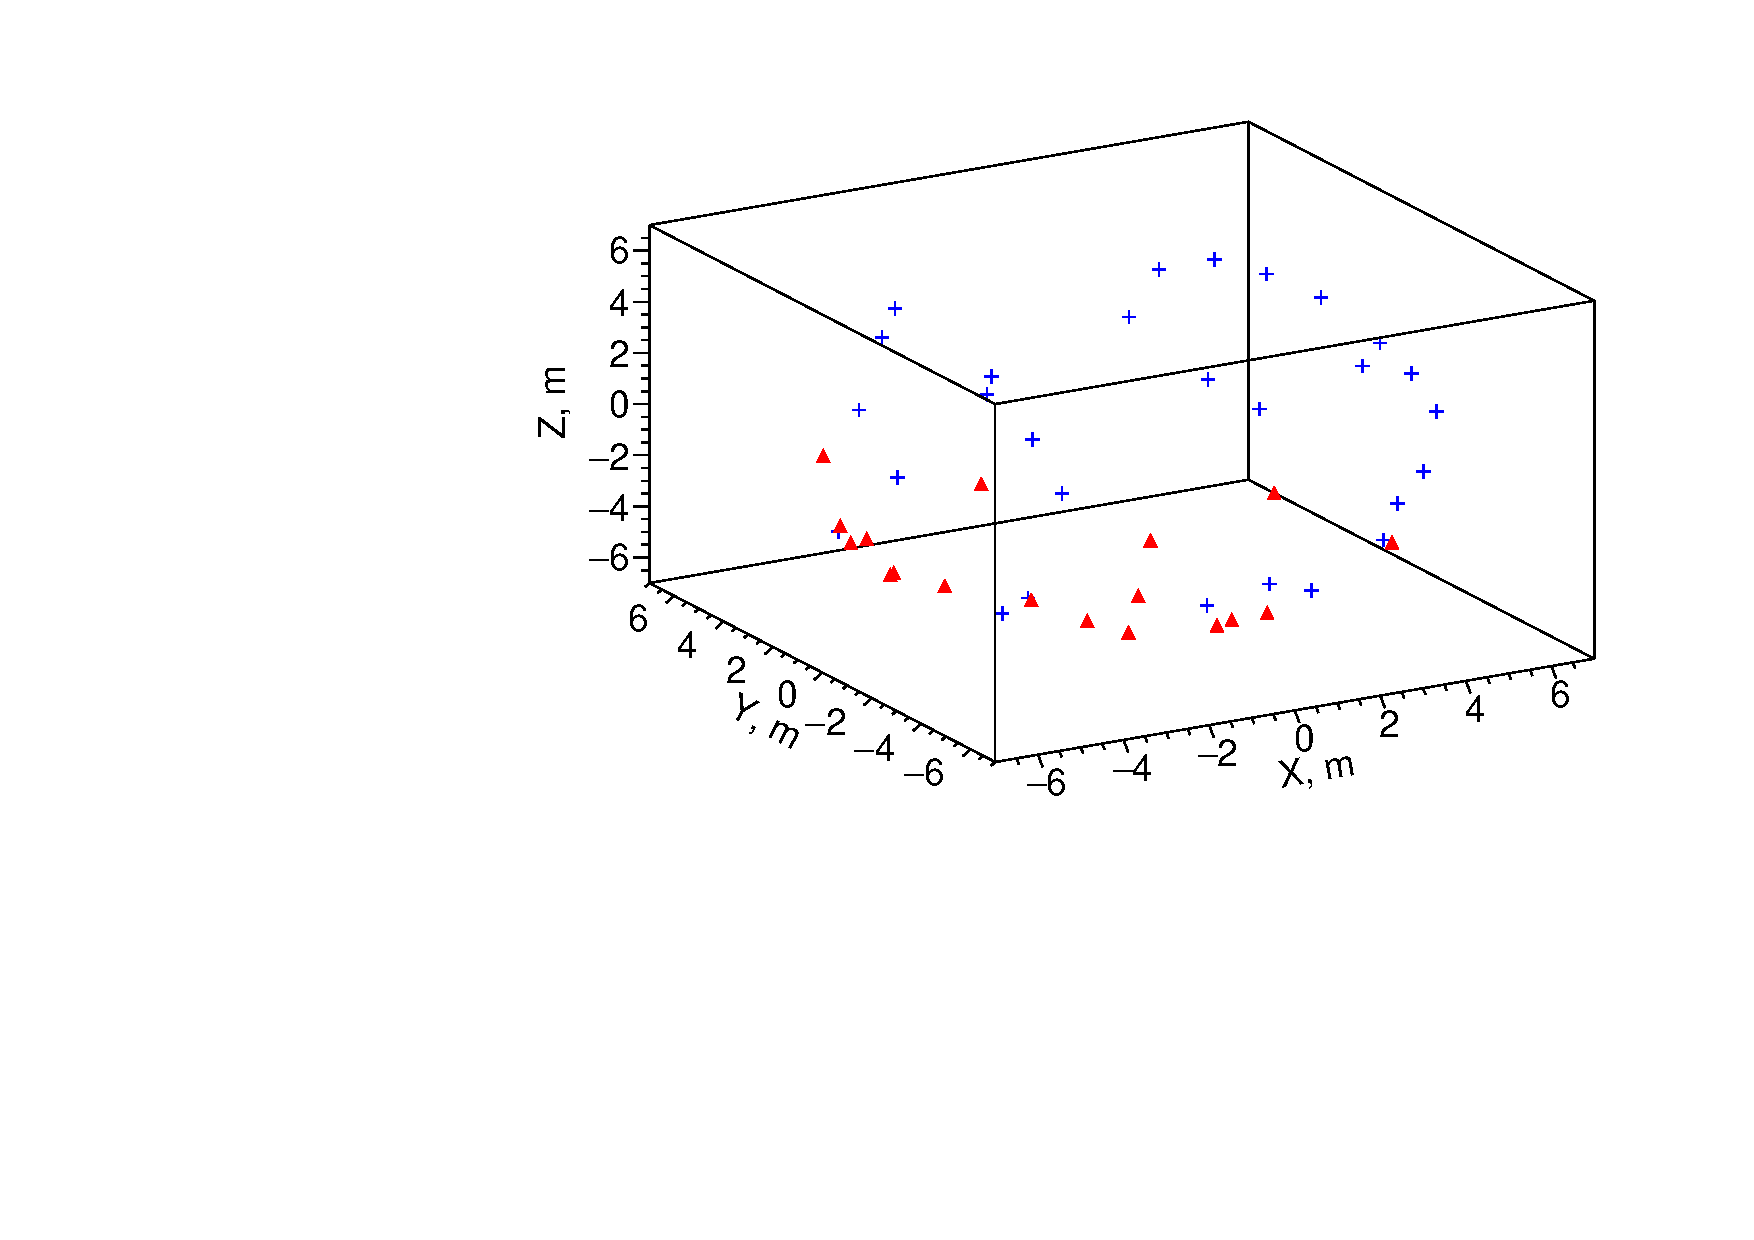
\includegraphics[angle=0,width=0.45\textwidth]{plots/hDisplay_Te130_evt352_e1186_e1340_cos0888}
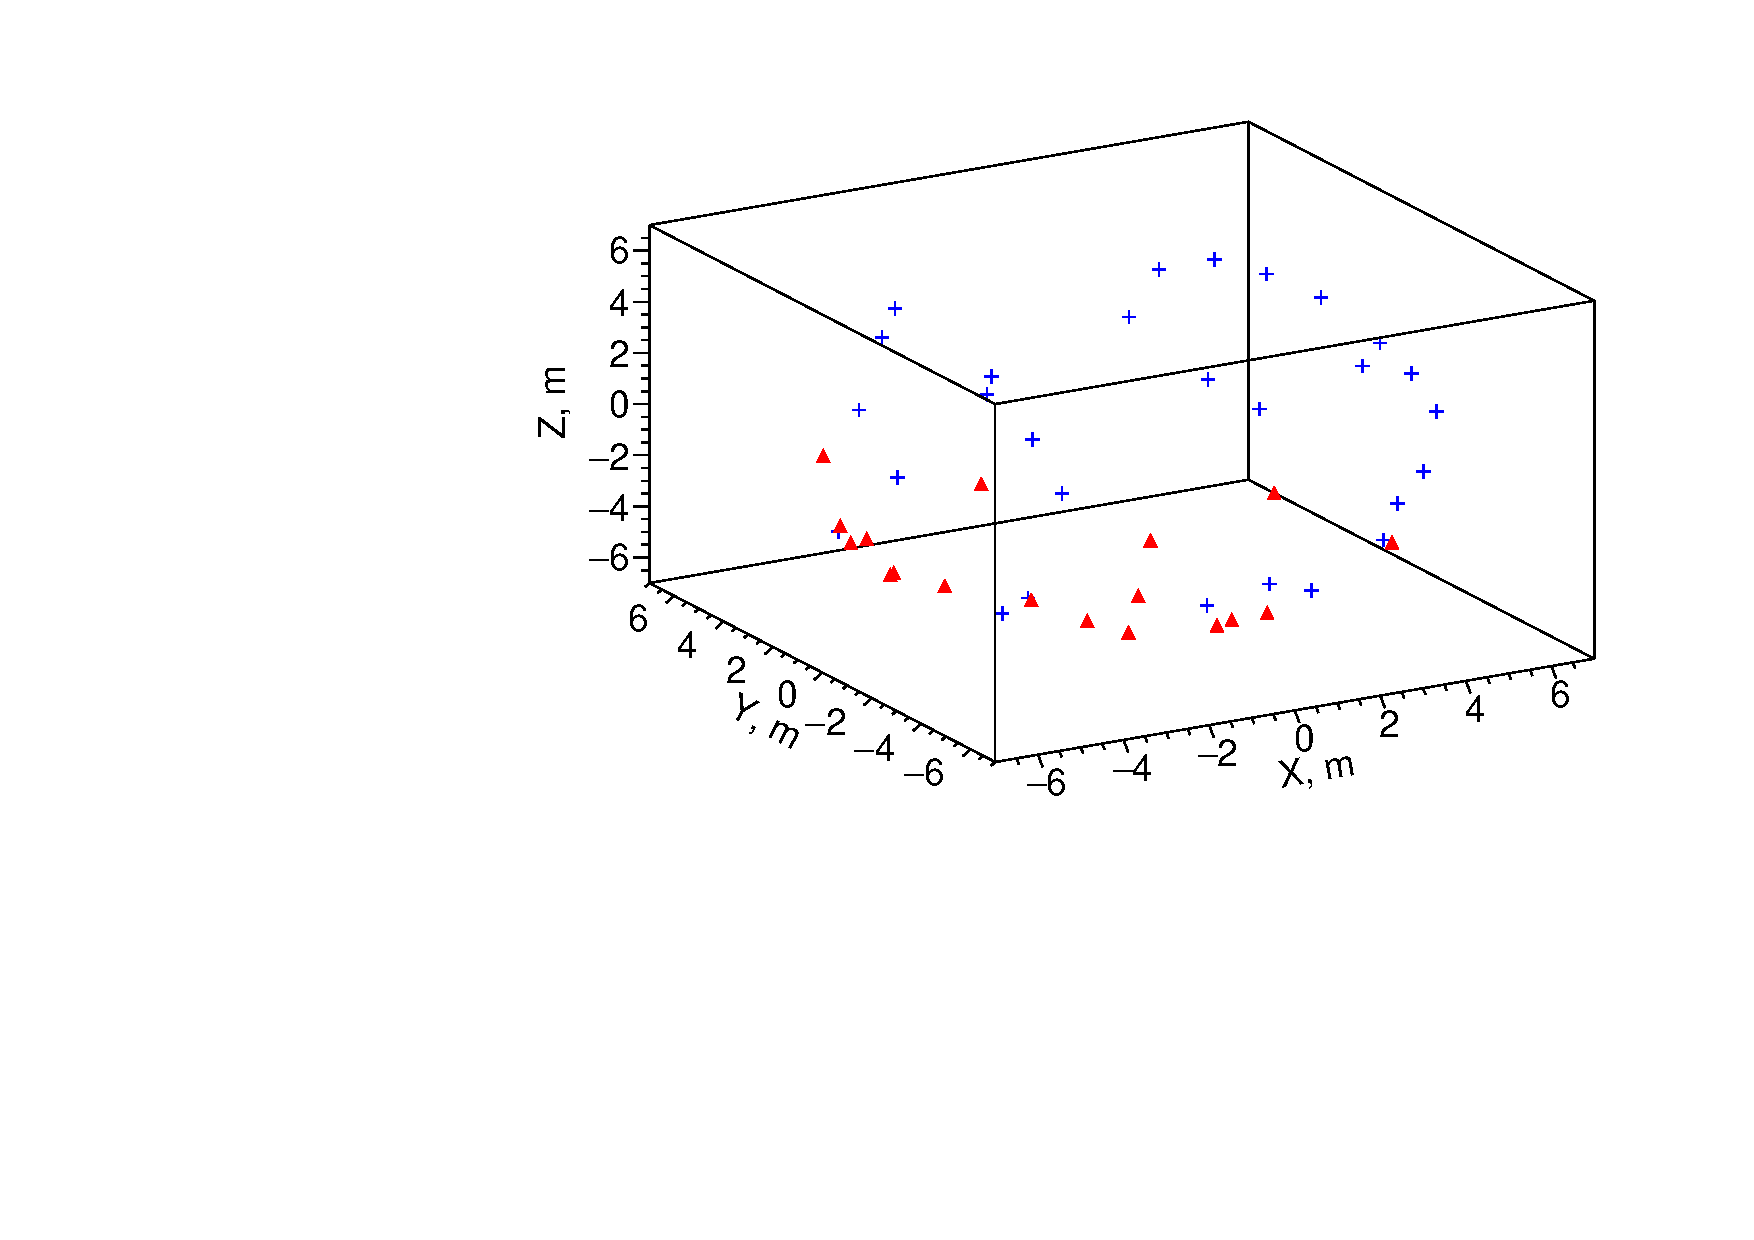
\includegraphics[angle=0,width=0.45\textwidth]{plots/hDisplay_Te130_evt352_e1186_e1340_cos0888}
\caption{Examples of PEs position on the detector sphere after time cut of 33.5ns. PEs from Cherenkov (red) and scintillation light (blue) are compared. (Top left) $\Te$ $\vbb$-decay back-to-back electrons: E$_1$=1.257~MeV, E$_2$=1.270~MeV, cos($\theta$)=-0.908. (Top right) $\Te$ $\vbb$-decay electrons at $\sim$90$^{\circ}$:  E$_1$=1.264~MeV, E$_2$=1.263~MeV, cos($\theta$)=-0.029. (Bottom left) $\Te$ $\vbb$-decay electrons at $\sim$0$^{\circ}$:  E$_1$=1.186~MeV, E$_2$=1.340~MeV, cos($\theta$)=0.888. (Bottom right) 2.529~MeV single electron. Events are simulated at the center of the detector. Default QE is applied.}
\label{fig:Display_Te130}
\end{figure}


%$\vbb$-decay events become indistinguishable from single track topology when the angle between two electrons is small
For quantitative description of the difference in the event topology we analyze spherical harmonics of the photon distributions on the detector sphere. We construct rotation invariant variables and compare them between signal and background events. As it is shown in the bottom part of Fig.~\ref{fig:Display_Te130} $\vbb$-decay become indistinguishable from single track topology when the angle between two electrons is small (two degenerate tracks). Event topologies of $\vbb$-decay and $\B$ events are also very similar when only one electron from $\vbb$-decay is above the Cherenkov threshold. Therefore spherical harmonics analysis is most efficient for events with large angular separation between the two electrons and when both electrons are above Cherenkov threshold. 

In this paper we focus on topological difference between two tracks and single track events and do not make any attempt to use absolute directional information to suppress single track events  where direction of the track is consistent with the direction of solar neutrinos. Once a single track topology is established one can use a centroid method (see Ref.~\cite{Directionality}) to reconstruct directionality of the track (or two degenerate tracks) and suppress events that are aligned with the direction of $\B$ solar neutrinos.

\subsection{Description of Spherical Harmonics Analysis}
A function $f(\theta,\phi)$ can be decomposed to a sum of spherical harmonics:

\begin{eqnarray}
\label{eq1}
f(\theta,\phi) = \sum_{l=0}^{\infty} \sum_{m=-l}^{l} f_{lm} Y_{lm}(\theta,\phi),
\end{eqnarray}

where $Y_{lm}$ are Laplace's spherical harmonics defined in real-value basis using Legendre polynomials $P_l$:

\begin{eqnarray}
\label{eq2}
Y_{lm} = LONGformulaHERE,
\end{eqnarray}

 where  coefficients $f_{lm}$ are defined as
 
\begin{eqnarray}
\label{eq3}
f_{lm} = LONGformulaHERE.
\end{eqnarray}

Equation~\ref{eq4} defines power spectrum of $f(\theta,\phi)$ in spherical harmonics representation, $s_l$, where $l$ is a multiple moment. The power spectrum $s_l$ is invariant under rotation. It is unique to each of the functions $f_i(\theta,\phi)$, $i=$1,2,3..., that can not be transformed into each other by rotation.

\begin{eqnarray}
\label{eq4}
s_l = \sum_{m=-l}^{m=l} |f_{lm}|^2
\end{eqnarray}

One can consider PEs distribution for each of $\vbb$-decay signal or background event as a function $f_i(\theta,\phi)$. Events with similar power spectrum would correspond to PE distributions on the detector sphere that can be closely aligned by a rotation. Such PE distributions belong to events with similar topology.

Topology of $\vbb$-decay signal or background in a spherical detector determines the distribution of the PE's on the detector sphere and therefore a set of $s_l$'s can serve as a quantitative figure of merit for different event topologies. Rotation invariance of $s_l$'s ensures that this figure of merit does not depend on the orientation of the event with respect to the chosen coordinate frame.


Sum of $s_l$'s over all multiple moments equals to L2 norm of the function $f(\theta,\phi)$:

\begin{eqnarray}
\label{eq5}
\sum_{l=0}^{\infty} s_l = \int_{\Omega} |f(\theta,\phi)|^2 d\Omega.
\end{eqnarray}

Therefore normalized power spectrum 

\begin{eqnarray}
\label{eq5}
S_l = \frac{s_l}{\sum_{l=0}^{\infty} s_l} =  \frac{s_l}{\int_{\Omega} |f(\theta,\phi)|^2 d\Omega}
\end{eqnarray}

can be used to compare shapes of various functions $f(\theta,\phi)$ with different normalization. The total number of PEs detected on the detector sphere fluctuates from event to event, therefore in all of the following we use normalized power $S_l$.

Figure~\ref{fig:Moments} compares normalized power spectrum for the three representative event topologies that have been already shown in Fig.~\ref{fig:Display_top_5MeV}. We note that most of the information contains in the power spectrum with $l<$6. In most cases we found that there is no need to calculate $S_l$ for $l>$3 to achieve maximal separation between $\vbb$-decay and $\B$ events, because fluctuations in the PE distribution produce a lot of noise in the power spectrum for higher orders of multiple moments.

\begin{figure}[htb]
\centering
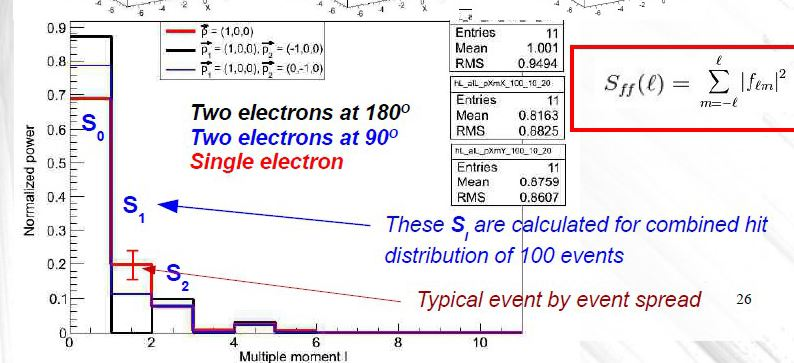
\includegraphics[angle=0,width=0.95\textwidth]{plots/Multiple_moment.JPG}
\caption{Average S$_l$ values for two electrons at 180 degree (color1) and 90 degree (color2) 1.5~MeV each and a single electron (color3) with the energy of 3~MeV. Error bars are RMS values of each corresponding individual S$_l$ distribution (each consists of 1000 events simulated at the center of the detector) indicating typical event-by-event variation.}
\label{fig:Moments}
\end{figure}




\subsection{Spherical Harmonics Analysis and Off-center Events}

In order to compare spherical harmonics for events with vertices located off-center anywhere inside the detector volume a coordinate transformation for each photon hit is needed. The necessary transformation applied for each PE within an event is illustrated in Fig.~\ref{fig:SphH_transform}. Solid circle with radius R schematically shows actual detector boundaries. Dotted circle shows a new sphere with the same radius R, which now has the event vertex in its center. The radius vector of each PE is stretched or shorten to its intersection with this new sphere using transformation $\vec{r}^{,}_{PE} = \frac{\vec{a}}{|\vec{a}|} \cdot R$. Where $\vec{r}^{,}_{PE}$ is a new radius vector of a PE and $\vec{a}=\vec{r}_{PE} - \vec{r}_{vtx}$ with $\vec{r}_{PE}$ and $\vec{r}_{vtx}$ being radius vectors of the PE and the vertex in the original coordinates respectively.

\begin{figure}[htb]
\centering
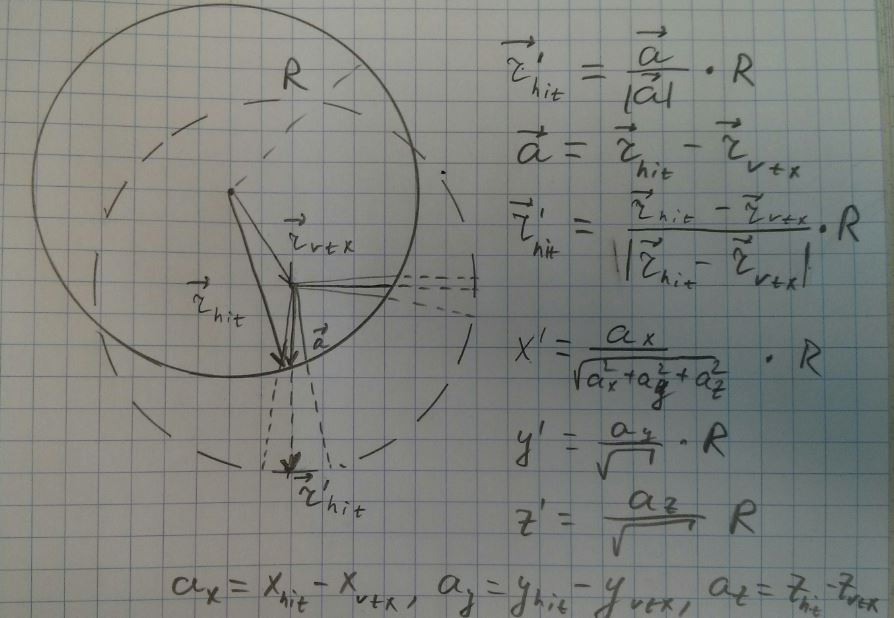
\includegraphics[angle=0,width=0.95\textwidth]{plots/SphH_transform_sketch.JPG}
\caption{Coordinate transformation applied to events that are off-center. Solid circle with radius R schematically shows actual detector boundaries. Dotted circle shows a new sphere with the same radius R, which now has the event vertex in its center. The radius vector of each PE is stretched or shorten to its intersection with this new sphere using transformation $\vec{r}^{,}_{PE} = \frac{\vec{a}}{|\vec{a}|} \cdot R$. Where $\vec{r}^{,}_{PE}$ is a new radius vector of a PE and $\vec{a}=\vec{r}_{PE} - \vec{r}_{vtx}$ with $\vec{r}_{PE}$ and $\vec{r}_{vtx}$ being radius vectors of the PE and the vertex in the original coordinates respectively.}
\label{fig:SphH_transform}
\end{figure}


\subsection{Implementation of the spherical harmonics analysis}
{\bf A few words on the implementation. Calculation of $S_l$'s requires numerical integration that needs to be explained.}

To illustrate spherical harmonics analysis technique we compare distributions of $S_0$, $S_1$, $S_2$, and $S_3$ for the three representative event topologies described in Sec.~\ref{subsec:topology}. Almost all the information about event topology is carried by Cherenkov light. Therefore we first show spherical harmonics for back-to-back,  90$^{\circ}$ and single track topologies based on Cherenkov PEs only (see Fig.~\ref{fig:SL_topologies_CHE}).

Two top panels of Fig.~\ref{fig:SL_topologies_CHE} show 2-dimensional distributions, S0 vs S1 and S2 vs S3, to demonstrate that all four $S_l$'s provide separation between event topologies. No QE is applied in simulation of these events. We also introduce a 1-dimensional variable, S01 (bottom panel of Fig.~\ref{fig:SL_topologies_CHE}), that has the best separation power for majority of event topologies considered in this paper. $S_{01}$ is defined as a projection of S$_1$ vs S$_2$ distribution onto a linear fit of this 2-D distribution.

\begin{figure}[htb]
\centering
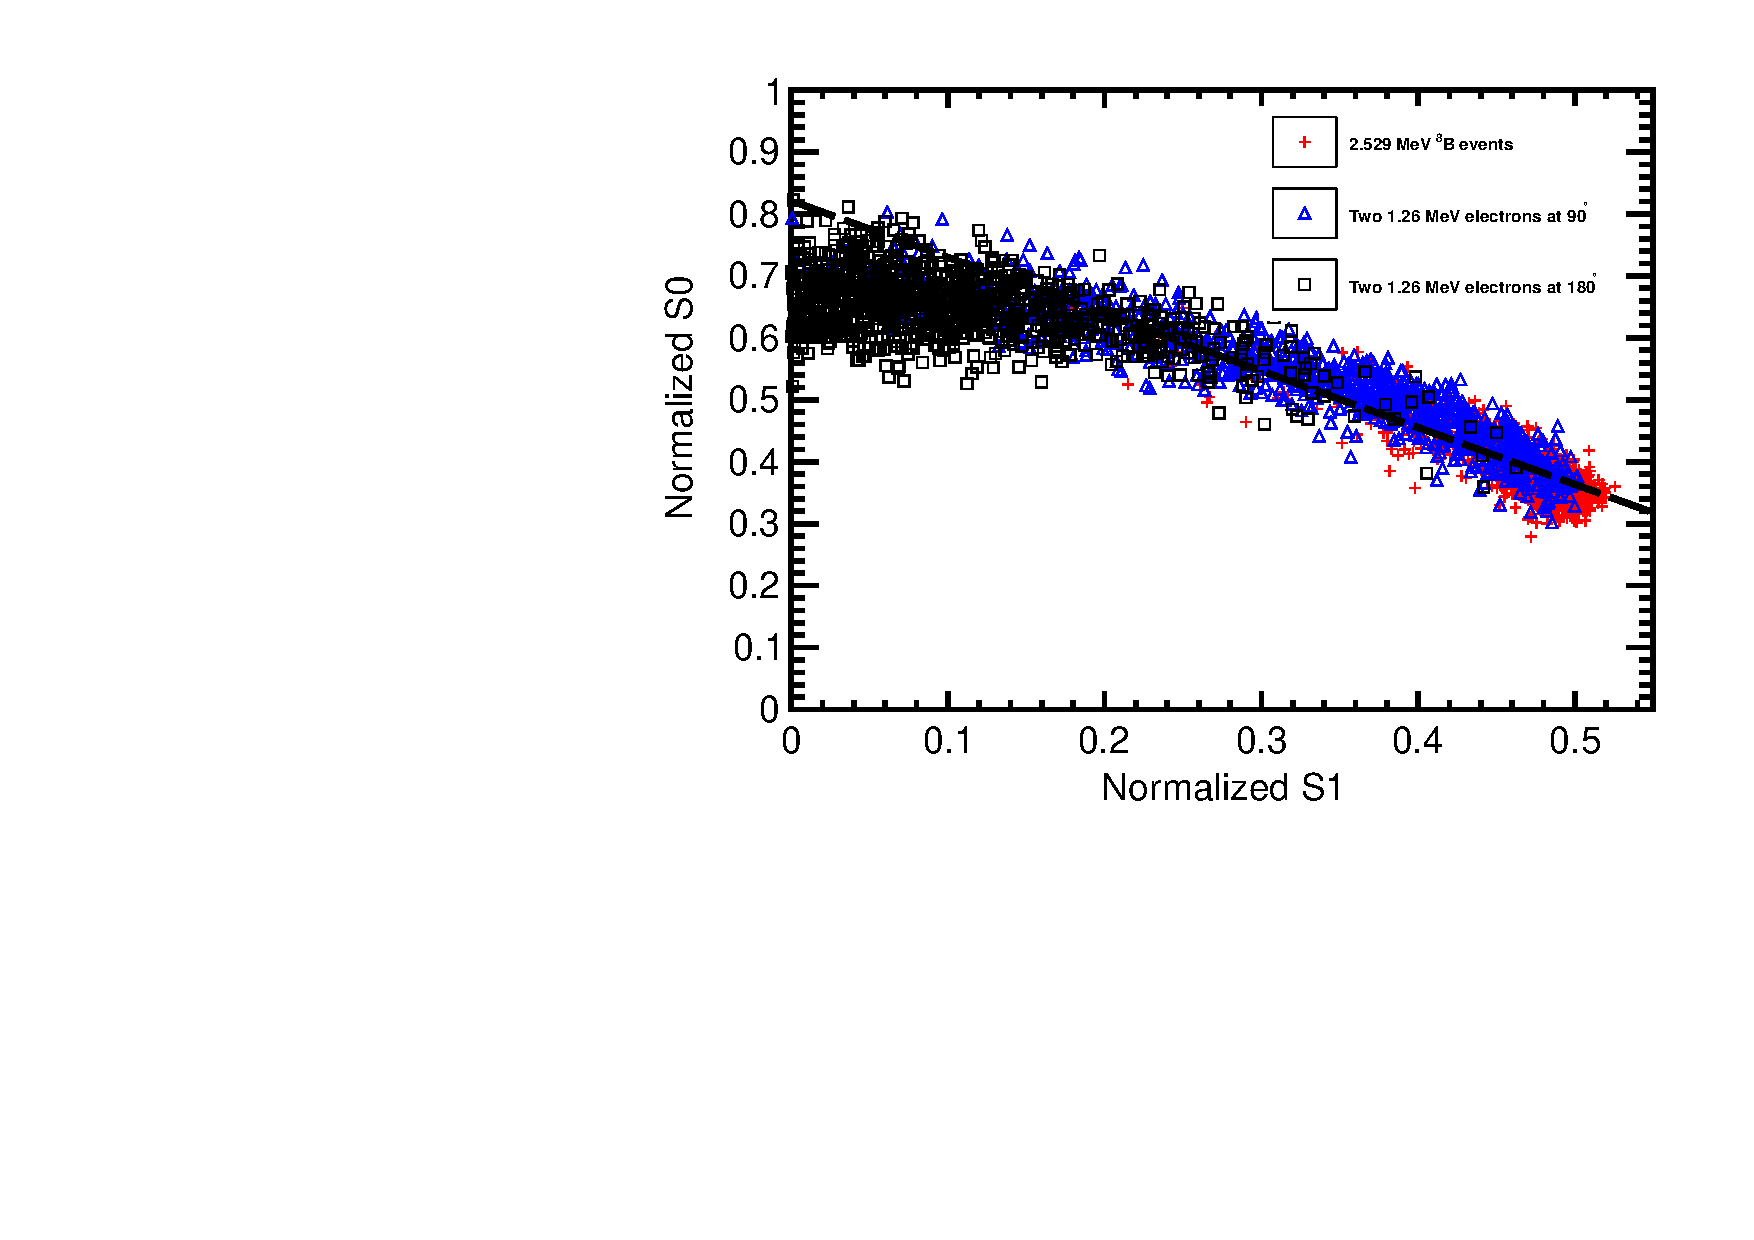
\includegraphics[angle=0,width=0.49\textwidth]{plots/ALL/hS0vsS1_topologies_CHELight_VtxSmear0cm_VtxShiftX0cm_33p5ns_center.pdf}
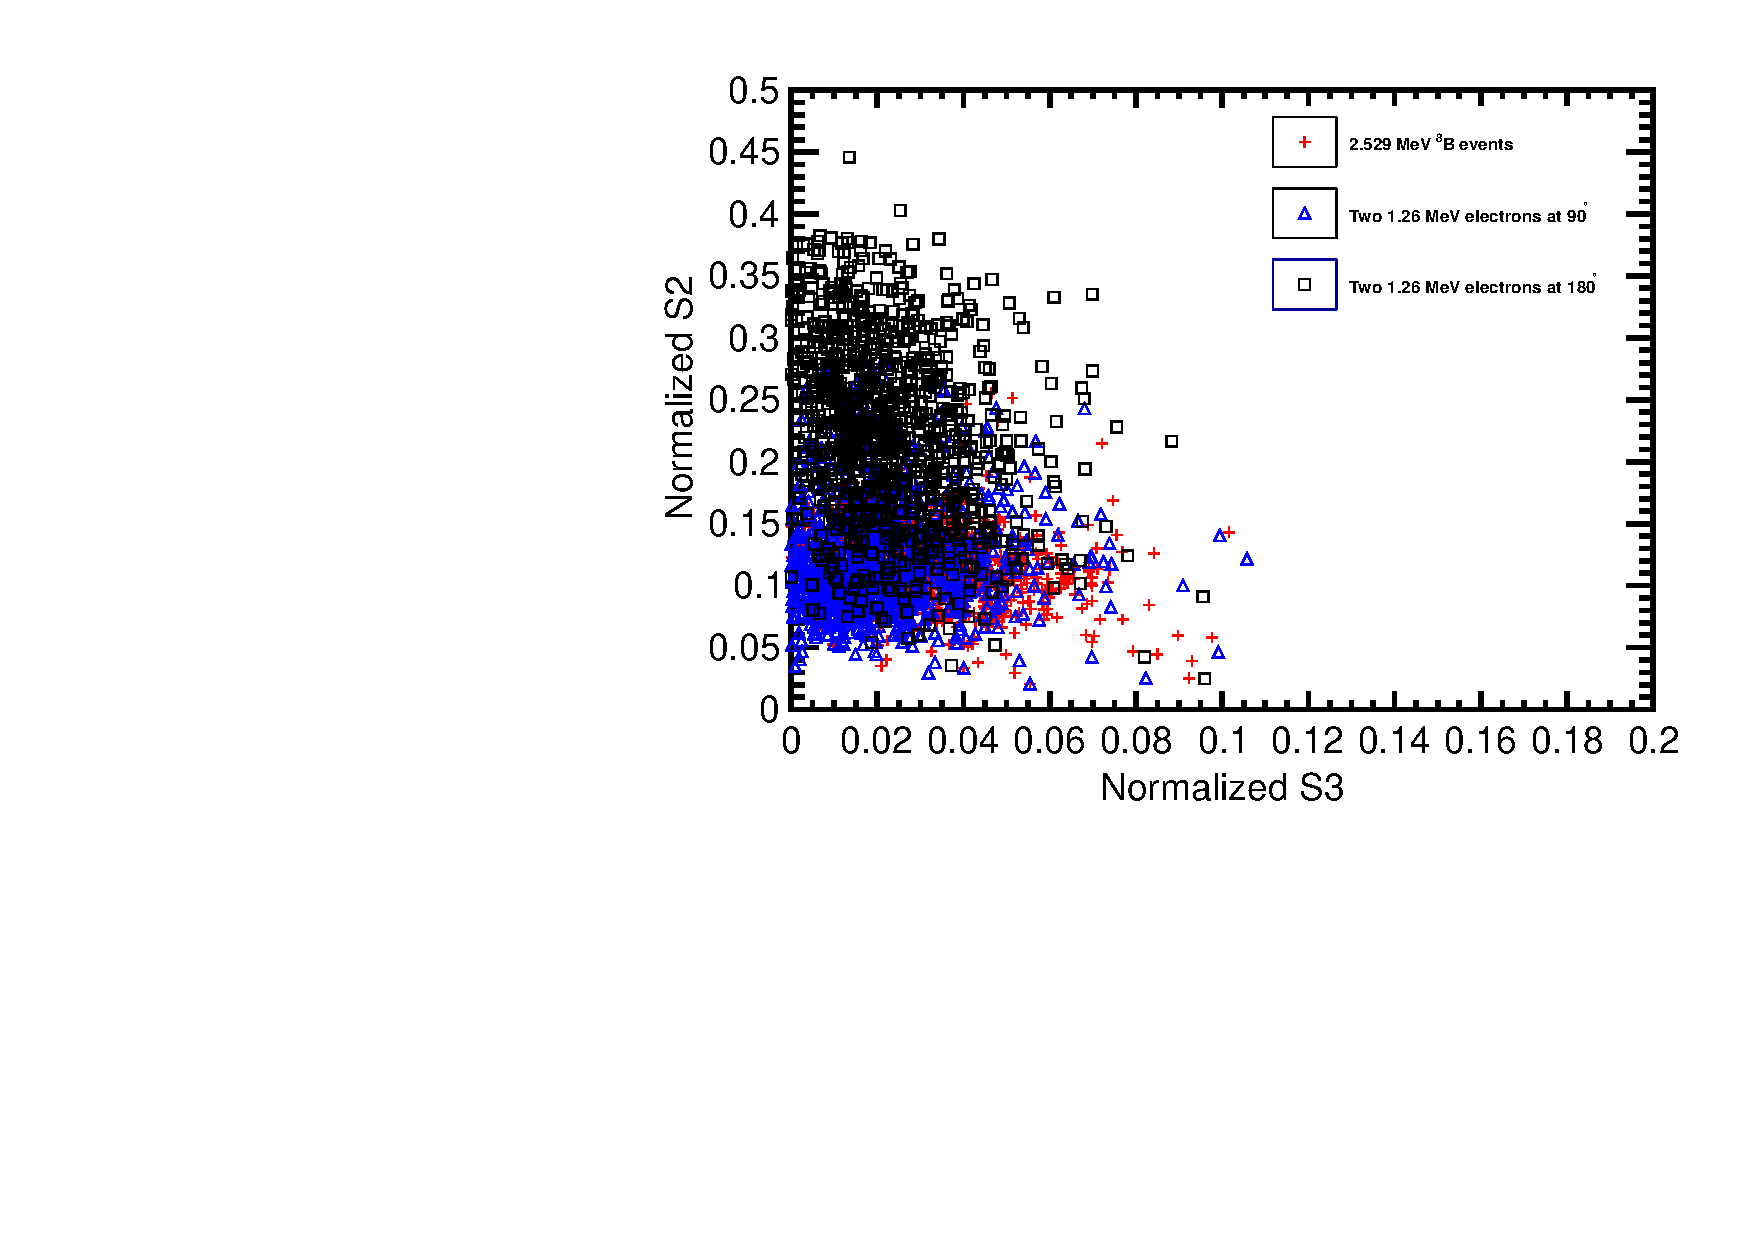
\includegraphics[angle=0,width=0.49\textwidth]{plots/ALL/hS2vsS3_topologies_CHELight_VtxSmear0cm_VtxShiftX0cm_33p5ns_center.pdf}
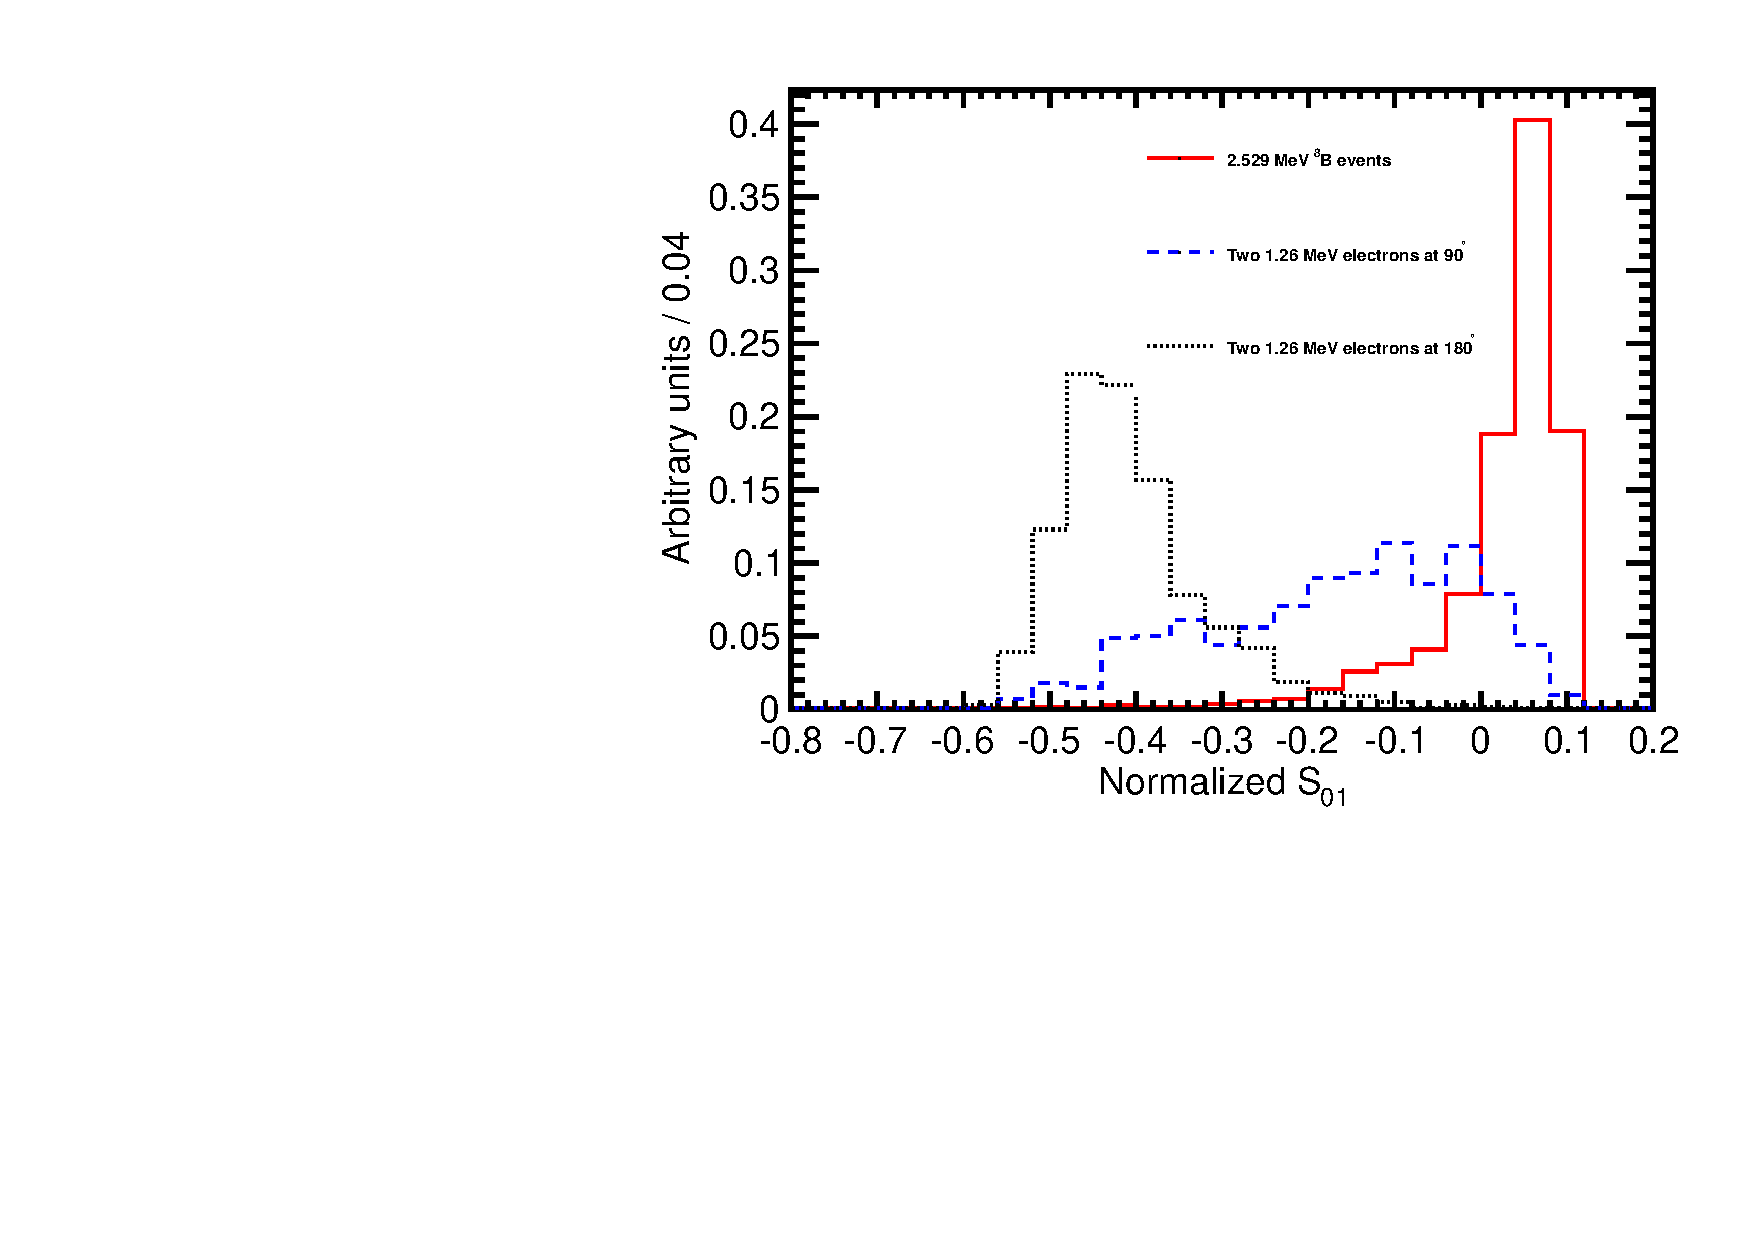
\includegraphics[angle=0,width=0.9\textwidth]{plots/ALL/hS01_topologies_CHELight_VtxSmear0cm_VtxShiftX0cm_33p5ns_center.pdf}
\caption{Spherical harmonics for three event topologies: two back-to-back 1.26~MeV electrons (black squares and black dotted line), two 1.26~MeV electrons at 90$^{\circ}$ angle (blue triangles and blue dashed line), and a single 2.529~MeV electron representing $\B$ background (red crosses and red solid line). Simulation of 1000 events originated at the center of the sphere. Perfect separation between Cherenkov and scintillation light is implemented in this simulation by using only Cherenkov photons. (Top left) S$_0$ versus S$_1$ scatter plot. Black dotted line is a linear fit of the 90$^{\circ}$ topology and $\B$ events. Variable S$_{01}$ is defined as a projection of 2D distribution onto this linear fit. (Top right) S$_2$ versus S$_3$ scatter plot. (Bottom) $S_{01}$ distributions for the three topologies. These distributions are normalized to unit area for shape comparison}
\label{fig:SL_topologies_CHE}
\end{figure}


The effects due to presence of scintillation light and applying default QE are shown in Fig.~\ref{fig:SL_topologies_all}. Spherical harmonics of the same three representative event topologies are now calculated using early light (photons with arrival time less than 33.5~ns) that contains both directional Cherenkov light and uniform scintillation light. Default QE is also applied. Higher order multiple moments, S2 and S3, no longer provide noticeable separation between different event topologies.


\begin{figure}[htb]
\centering
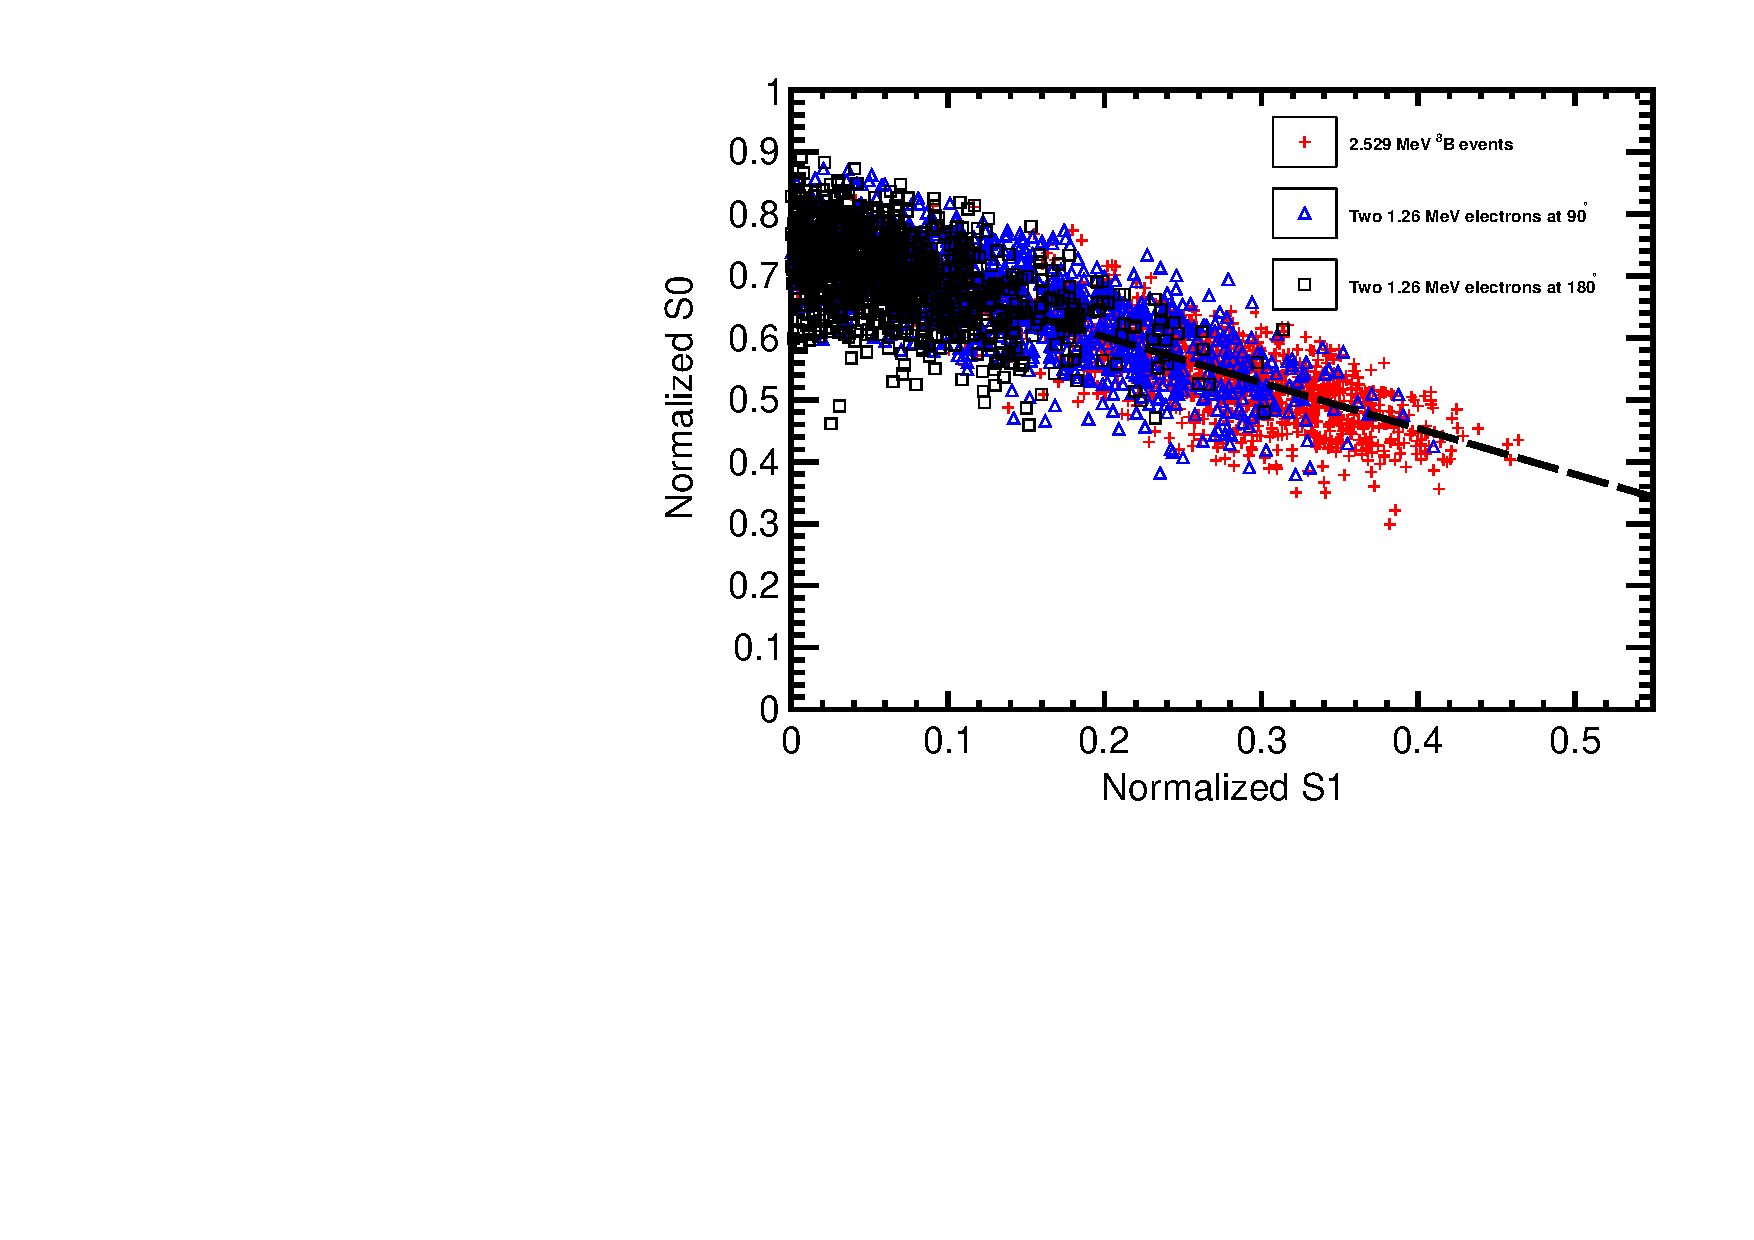
\includegraphics[angle=0,width=0.49\textwidth]{plots/hS0vsS1_topologies_allLight_VtxSmear0cm_VtxShiftX0cm_33p5ns_center.pdf}
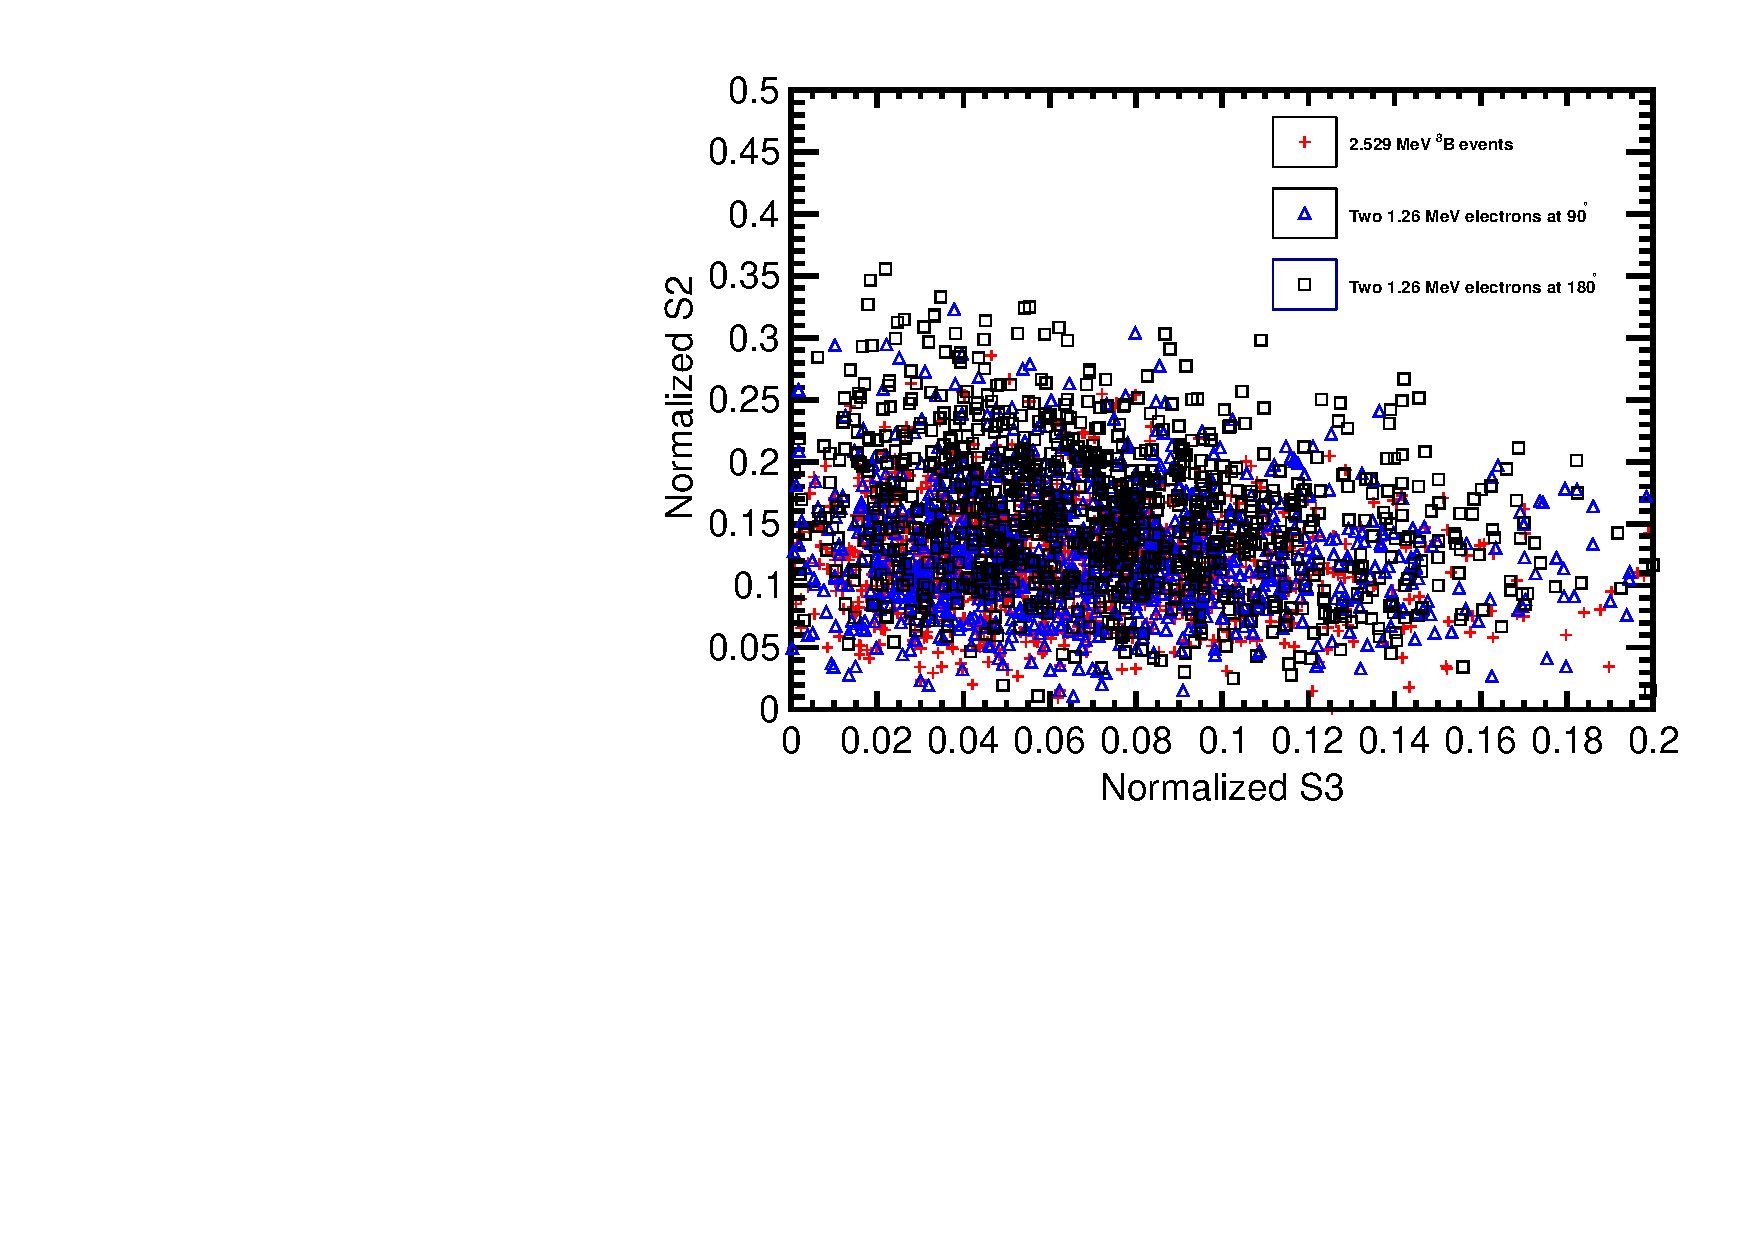
\includegraphics[angle=0,width=0.49\textwidth]{plots/hS2vsS3_topologies_allLight_VtxSmear0cm_VtxShiftX0cm_33p5ns_center.pdf}
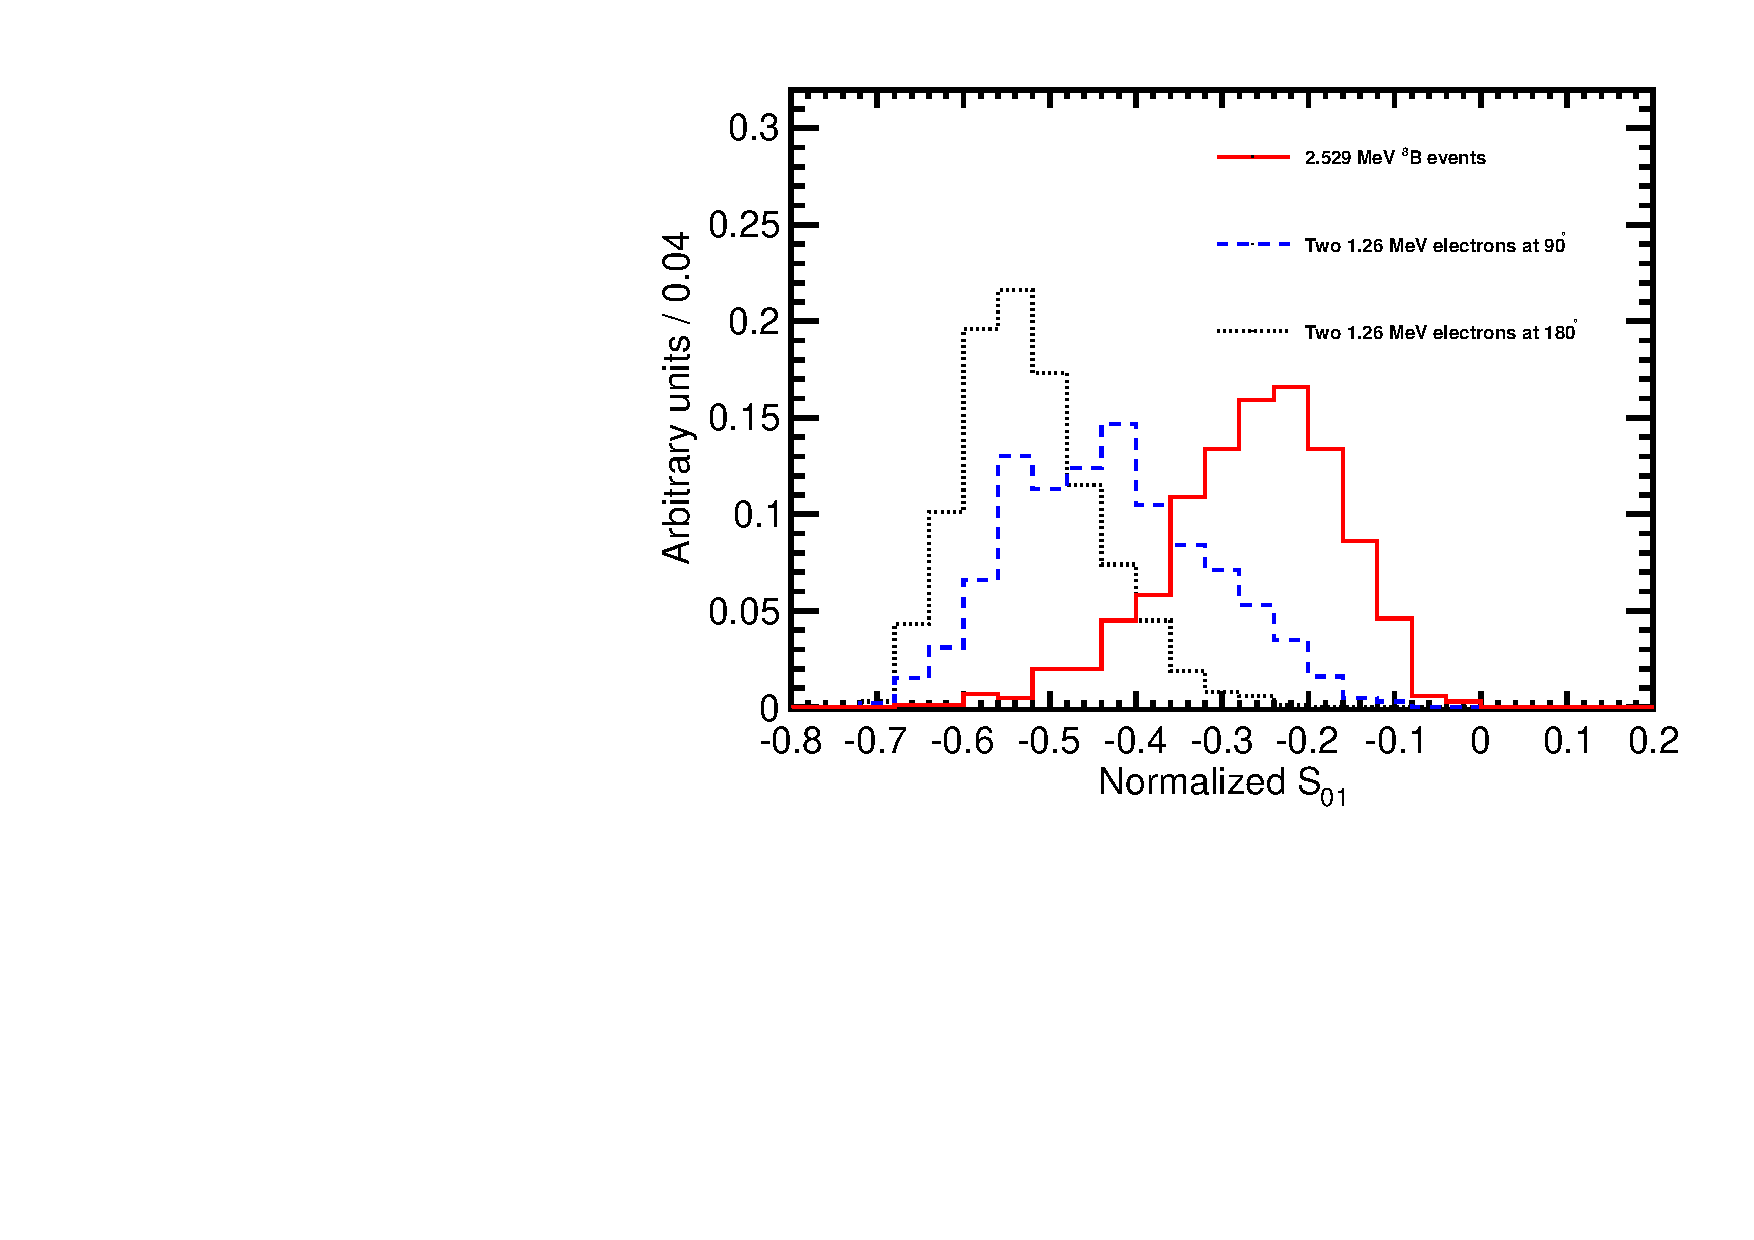
\includegraphics[angle=0,width=0.9\textwidth]{plots/hS01_topologies_allLight_VtxSmear0cm_VtxShiftX0cm_33p5ns_center.pdf}
\caption{Spherical harmonics for three event topologies: two back-to-back 1.26~MeV electrons (black squares and black dotted line), two 1.26~MeV electrons at 90$^{\circ}$ angle (blue triangles and blue dashed line), and a single 2.529~MeV electron representing $\B$ background (red crosses and red solid line). Simulation of 1000 events originated at the center of the sphere. Separation between Cherenkov and scintillation light is implemented 33.5~ns cut on the photon arrival time. Perfect vertex reconstruction - true vertex position is used. (Top left) S$_0$ versus S$_1$ scatter plot. Black dotted line is a linear fit of the 90$^{\circ}$ topology and $\B$ events. Variable S$_{01}$ is defined as a projection of 2D distribution onto this linear fit. (Top right) S$_2$ versus S$_3$ scatter plot. (Bottom) $S_{01}$ distributions for the three topologies. These distributions are normalized to unit area for shape comparison}
\label{fig:SL_topologies_all}
\end{figure}


\section{Performance and Experimental Challenges}
\label{sec:performance_and_challenges}

\subsection{Performance of the spherical harmonics analysis on $\vbb$-decay and $\B$ events.}

Comparison of $S_0$ and $S_1$ distributions between $\vbb$-decay and $\B$ events is shown in Fig.~\ref{fig:S_vs_energy}. There is a noticeable separation between the signal and background. We also note that in the energy range of interest $S_l$'s do not have strong dependence on the energy deposited in the detector, which makes them reliable discriminators at the end point of the $\vbb$-decay energy spectrum. The information about the event topology is complimentary to the energy measurements.

\begin{figure}[htb]
\centering
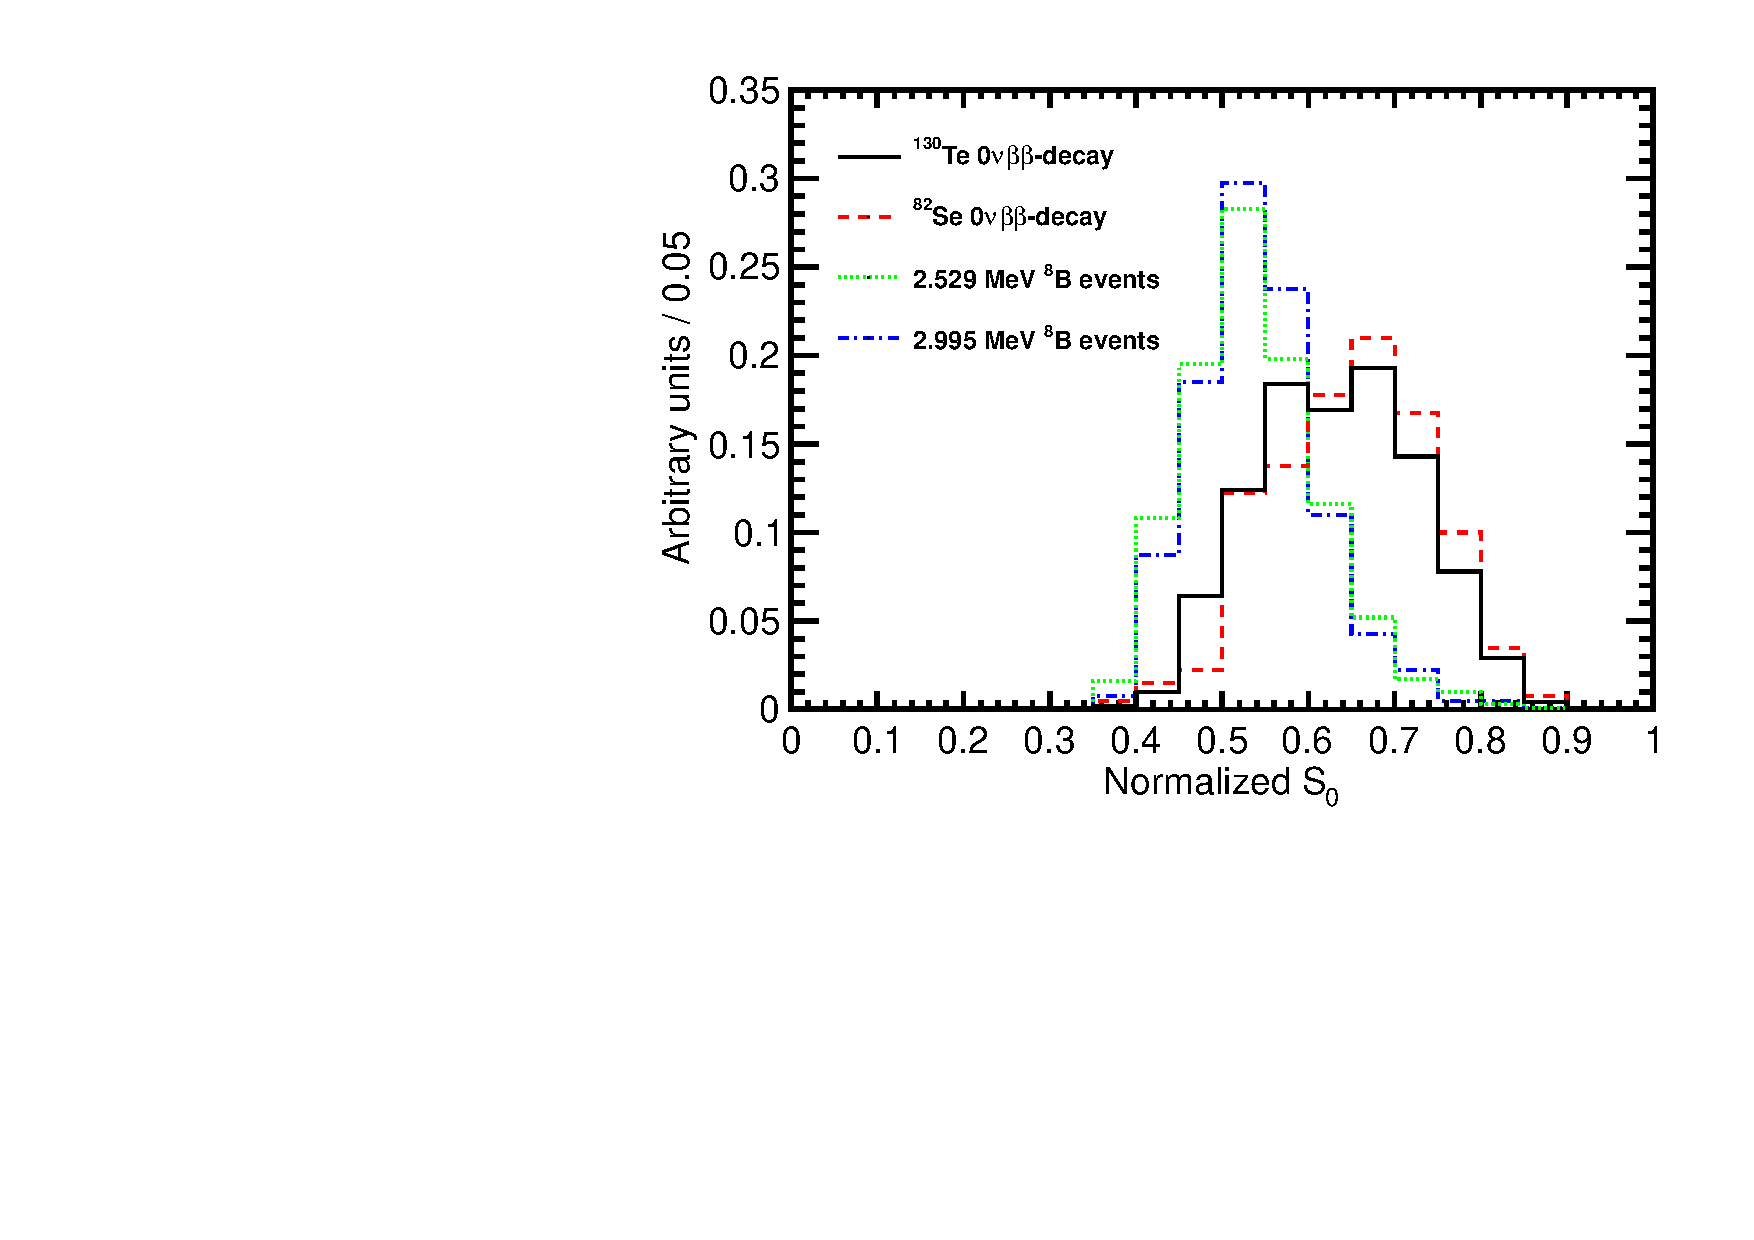
\includegraphics[angle=0,width=0.49\textwidth]{plots/hS0.pdf}
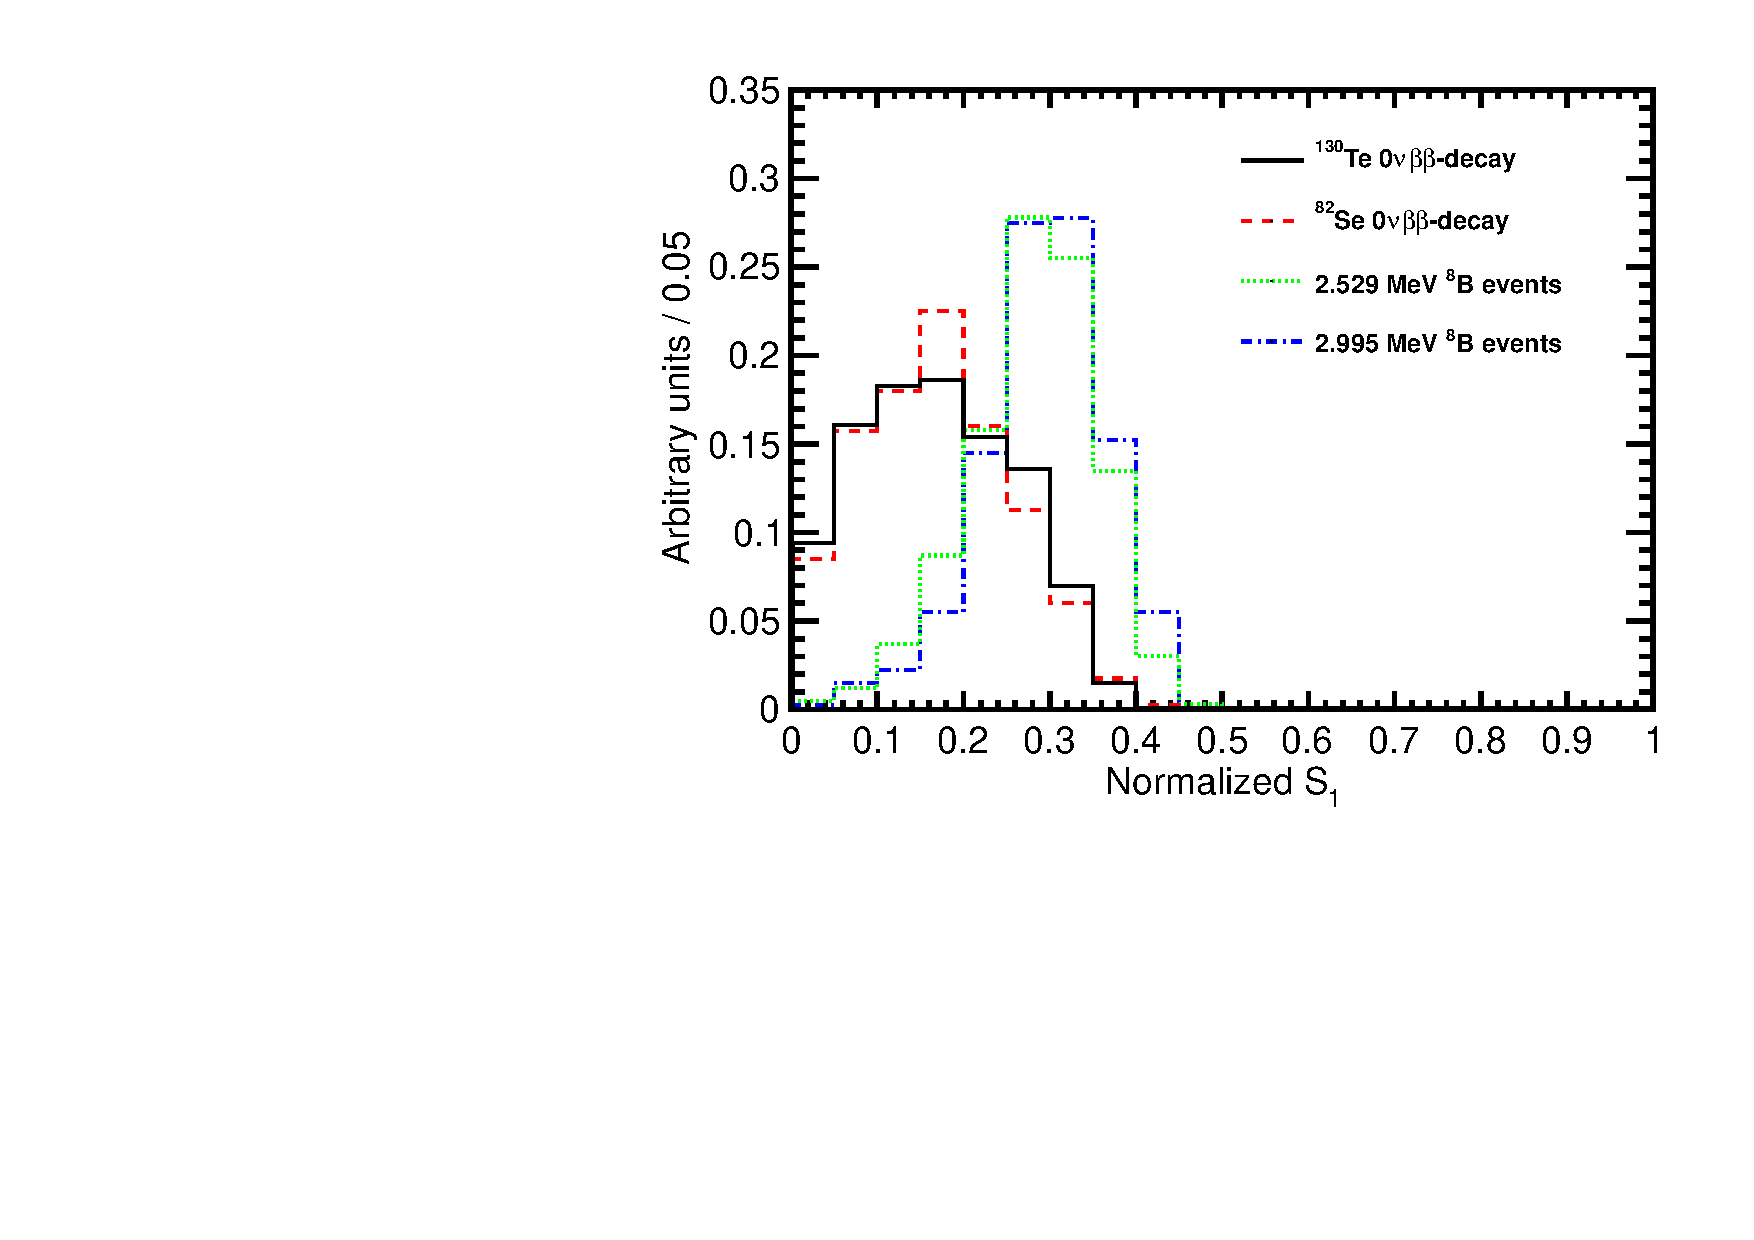
\includegraphics[angle=0,width=0.49\textwidth]{plots/hS1.pdf}
\caption{$S_0$ (left) and $S_1$ (right) distributions for events with two different event topologies and total kinetic energy. $^{130}Te$, $^{82}Se$ $\vbb$-decay, 2.529 MeV and 2.995 MeV events are compared. The simulation is done for events with the vertex in the center of the detector. $\B$ events are implemented as 2.529~MeV or 2.995~MeV electrons with initial direction along $x$-axis. Perfect vertex reconstruction - true vertex position is used. Time cut of 33.5~ns on the photon arrival time is applied.}
\label{fig:S_vs_energy}
\end{figure}


Figure~\ref{fig:SL_Te_33p5ns_center} shows separation between $\Te$ signal and $\B$ background events simulated at the center of the detector. True values of vertex position and time is used. Time cut of 33.5~ns on the photon arrival time is applied to separate Cherenkov and scintillation light. Most of the discrimination between signal and background comes from $S_0$ and $S_1$. In the following $S_2$ and $S_3$ are not used to separate $\Te$ and $\B$ events\footnote{$S_2$ and $S_3$ are helpful for separation of $\Te$ signal from $\Cten$ background. See Appendix.}. The scatter plot of $S_2$ vs $S_3$ is shown here for completeness. 

In order to optimize separation between $\Te$ signal and $\B$ background a linear combination of $S_0$ and $S_1$, $S_{01}$, is used. A linear fit, $S_0$ = $A \times S_1 + B$, of 2-dimensional $S_0$ vs $S_1$ scatter plot is performed as shown in Fig.~\ref{fig:SL_Te_33p5ns_center}. Then this 2-dimensional distribution is projected onto the fitted line. {\bf A little bit of math here to quantitatively describe $S_{01}$ via $S_0$ and $S_1$:} A new coordinate frame is obtained by rotation of the original $S_0$-$S_1$ frame at angle $\theta$ obtained from the fit: $tan(\theta)$=$A$. A transformation, $S_{01} = S_1 \cdot cos(\theta) + S_0 \cdot sin(\theta)$, defines the $S_{01}$ variable.

Bottom plot in Fig.~\ref{fig:SL_Te_33p5ns_center} shows performance of the $S_{01}$ variable to separate $\Te$ signal and $\B$ background. A fit to this distribution can be done to optimize the discrimination power in a particular experimental settings. Here we refrain from quantitative estimates on the improvements in sensitivity to $\vbb$-decay search using this method of spherical harmonics as a reliable estimate would require a dedicated analysis taking into account all the details of a particular experiment.

\begin{figure}[htb]
\centering
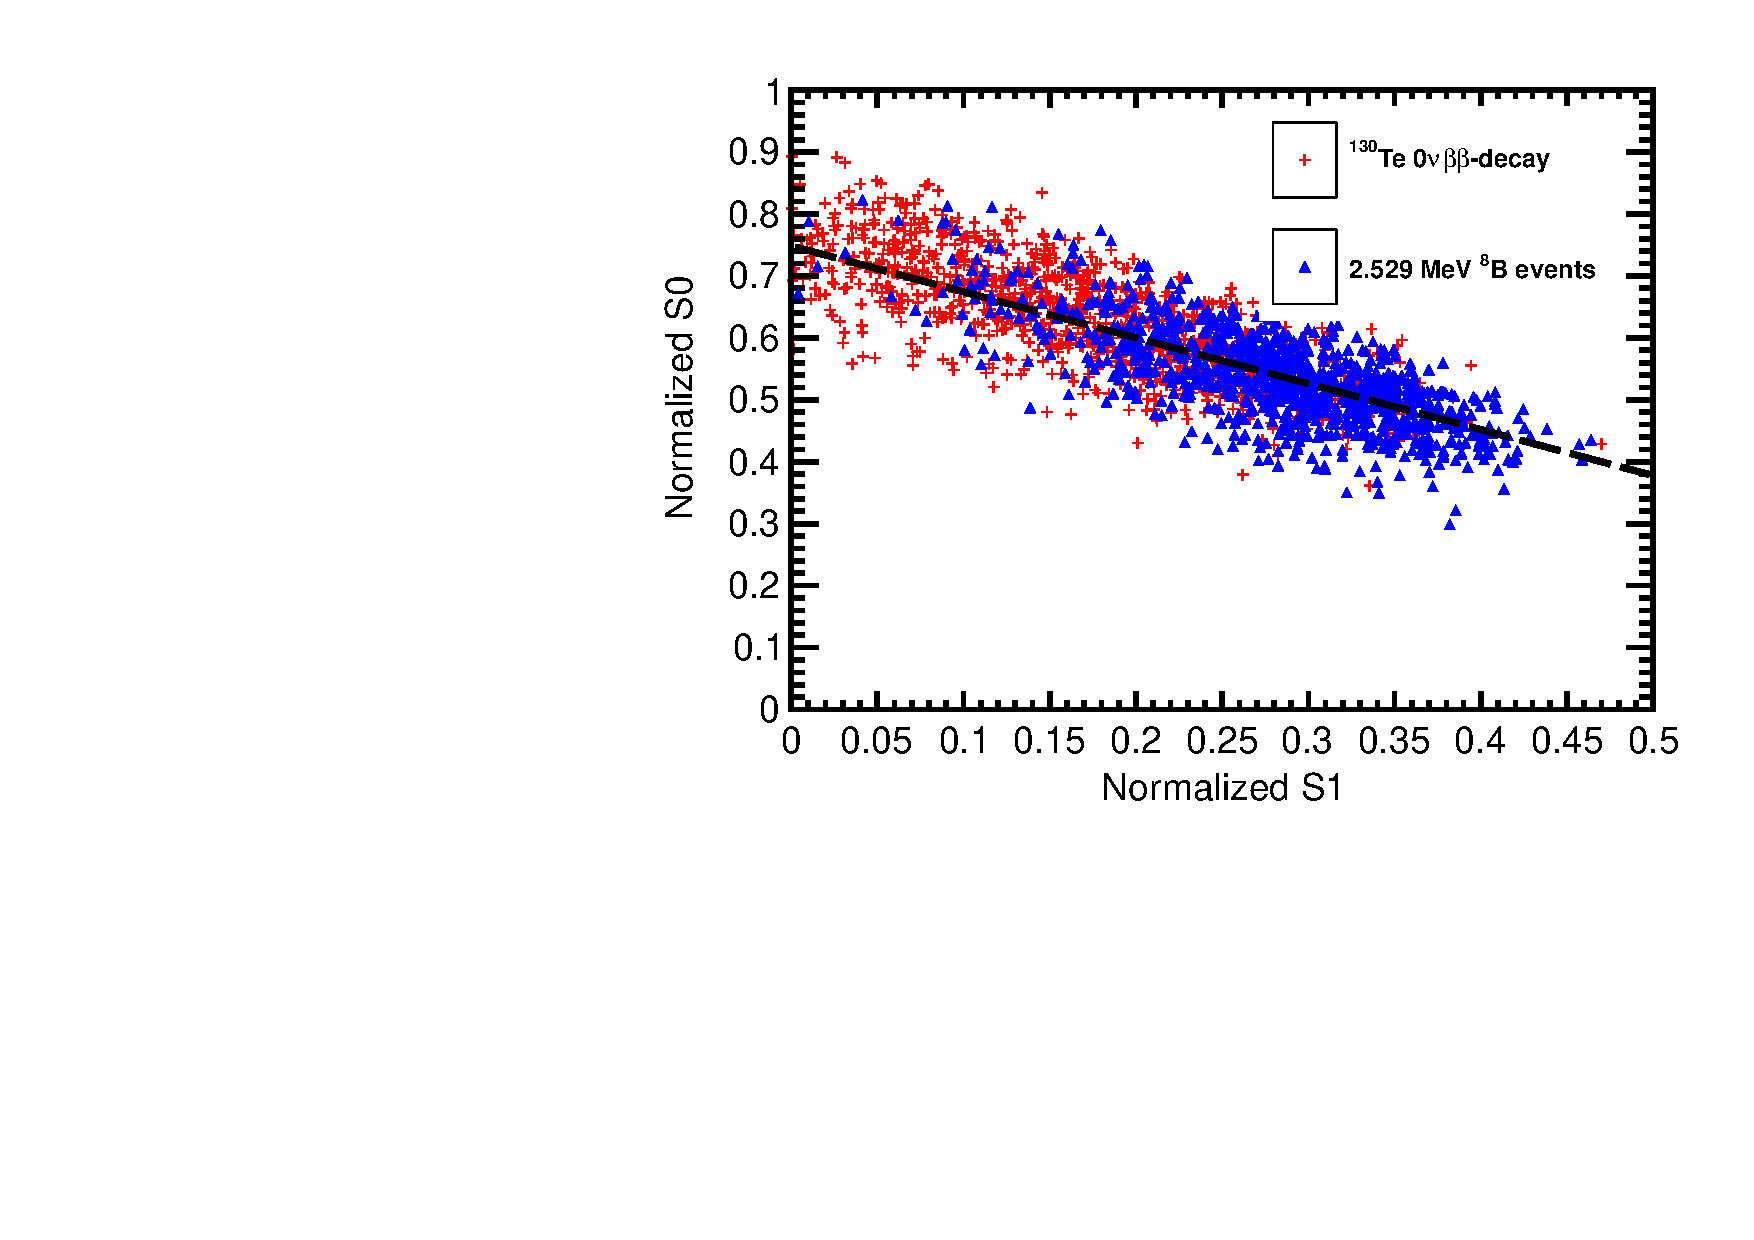
\includegraphics[angle=0,width=0.49\textwidth]{plots/hS0vsS1_Te130_1el_allLight_VtxSmear0cm_VtxShiftX0cm_33p5ns_center.pdf}
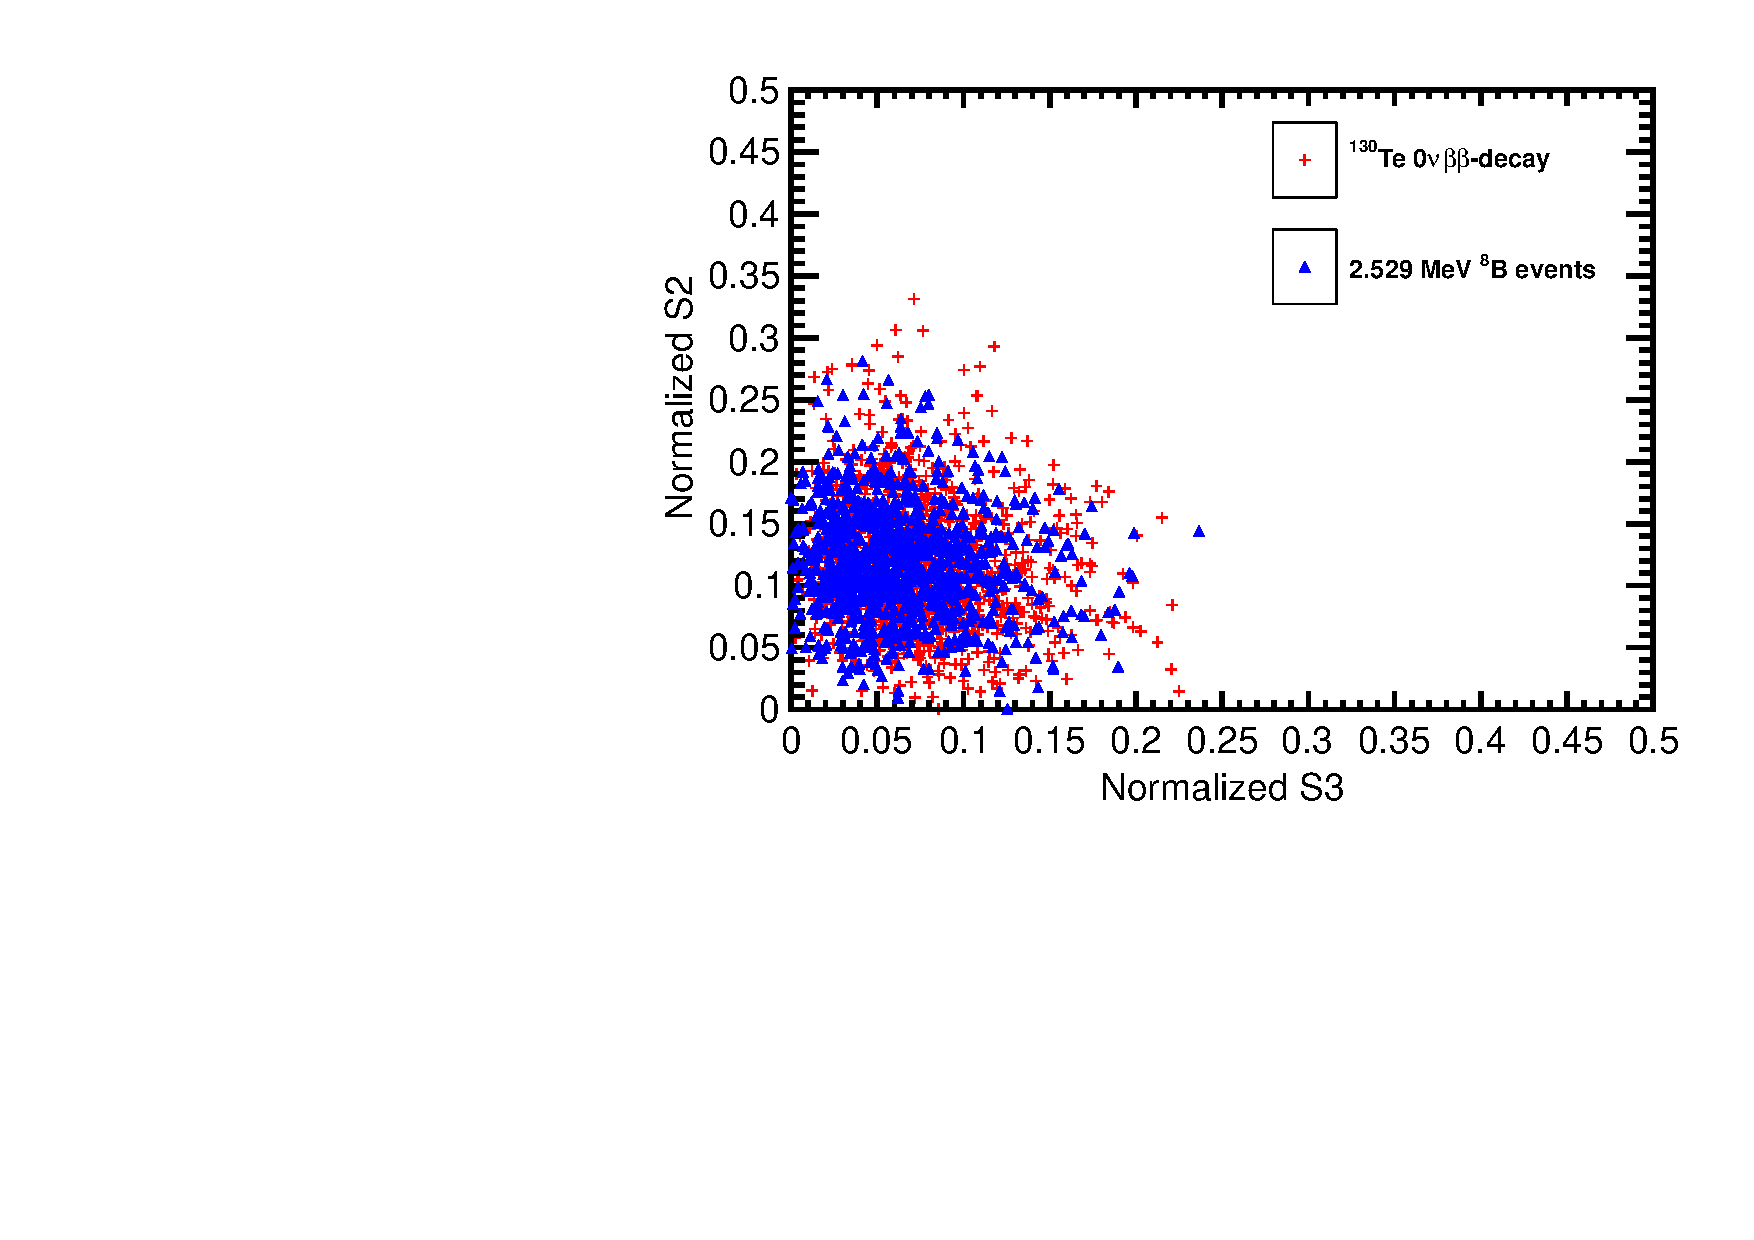
\includegraphics[angle=0,width=0.49\textwidth]{plots/hS2vsS3_Te130_1el_allLight_VtxSmear0cm_VtxShiftX0cm_33p5ns_center.pdf}
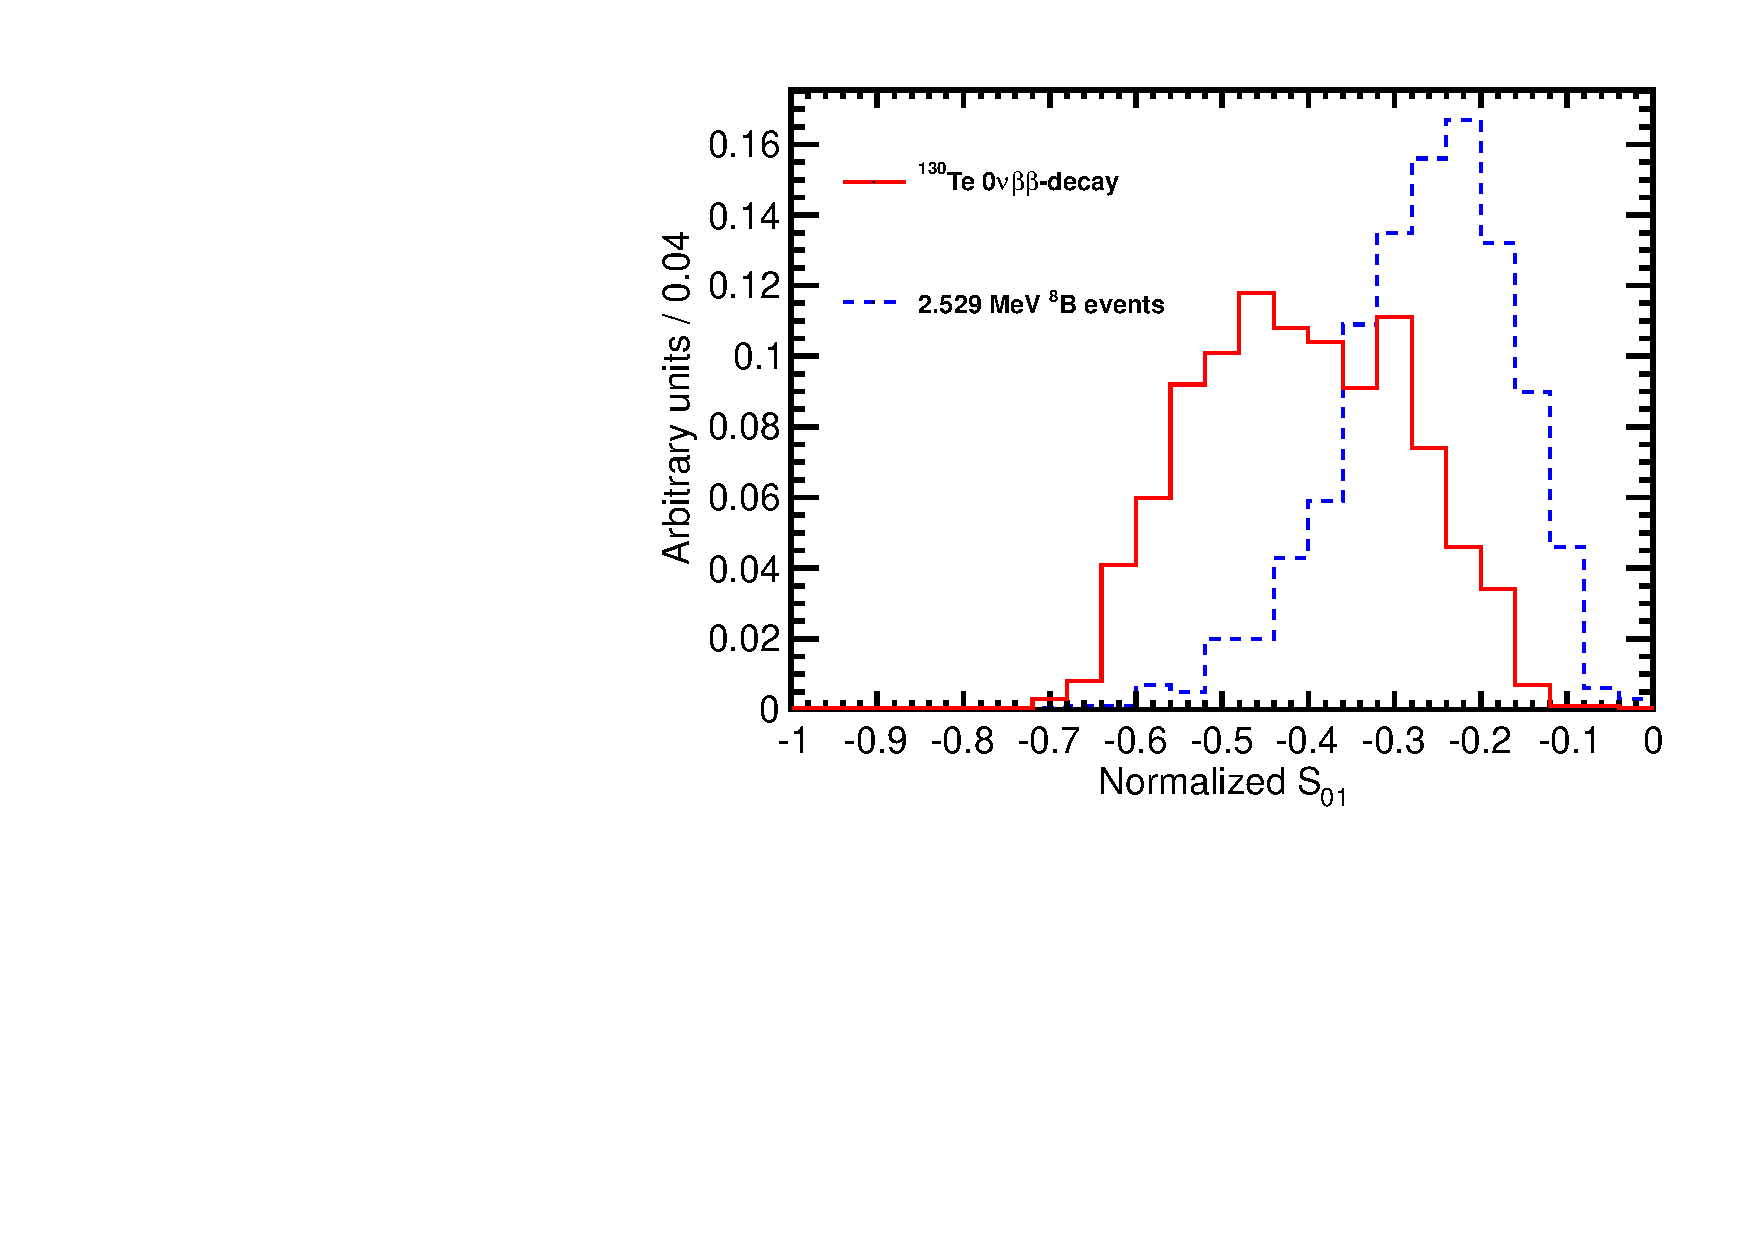
\includegraphics[angle=0,width=0.9\textwidth]{plots/hS01_allLight_VtxSmear0cm_VtxShiftX0cm_33p5ns_center.pdf}
\caption{Spherical harmonics comparison between $\Te$ $\vbb$-decay signal (Q$=$2.529~MeV) (red) and $\B$ solar neutrinos background (blue) for 1000 simulated events originated at the center of the sphere. $\B$ events are implemented as 2.529~MeV electrons with initial direction along $x$-axis. Perfect vertex reconstruction - true vertex position is used. Time cut of 33.5~ns on the photon arrival time is applied. (Top left) S$_0$ versus S$_1$ scatter plot. Black dotted line is a linear fit of these 2D histograms. Variable S$_{01}$ is defined as a projection of 2D distribution onto this linear fit. (Top right) S$_2$ versus S$_3$ scatter plot. (Bottom) $S_{01}$ distribution for the signal and background.}
\label{fig:SL_Te_33p5ns_center}
\end{figure}


\subsection{Experimental challenges}

So far only events at the center of the detector have been considered. In this section we discuss performance of the spherical harmonics analysis for events distributed within the fiducial volume of the detector taking into account finite resolution on vertex position reconstruction.

When the vertex is not at the center, a uniform time cut on the photon arrival time is no longer effective in the selection of Cherenkov photons. In the case of off-center vertex, even significantly delayed scintillation photons can reach the side of the detector that is closer to the vertex much earlier than Cherenkov photons traveling to the opposite side of the detector. Therefore, the time cut has to be position dependent and take into account the total distance traveled by each individual photon.

We found that the time cut defined as $\Delta t$=$t^{phot}_{measured} - t^{phot}_{predicted}$$<$1~ns selects photons with sufficient fraction of Cherenkov photons. Predicted time, $ t^{phot}_{predicted}$=$l/v^{phot}$, depends on total distance, $l$, traveled by the photon and proper assignment of the velocity for each photon, $v^{phot}$, that depends on index of refraction\footnote{We use average index of refraction of n=1.53}. Therefore the relative Cherenkov/scintillation composition of the light selected with this $\Delta t$ time cut depends on the vertex location and chromatic dispersions. 

Due to chromatic dispersion, even with perfect vertex reconstruction one cannot achieve the same level of separation between Chrerenkov and scintillation light compared to the central events considered above in Section 4. This in turn reduces the effectiveness of the spherical harmonics analysis in separating of $\vbb$-decay and $\B$ events (see Fig.~\ref{fig:SL_Te_SmearX0cm_momDT1ns_rndVtx_3p0m}). However next generation detectors can recover losses due to chromatic dispersion by choosing liquid scintillators with a more narrow emission spectrum.


\begin{figure}[htb]
\centering
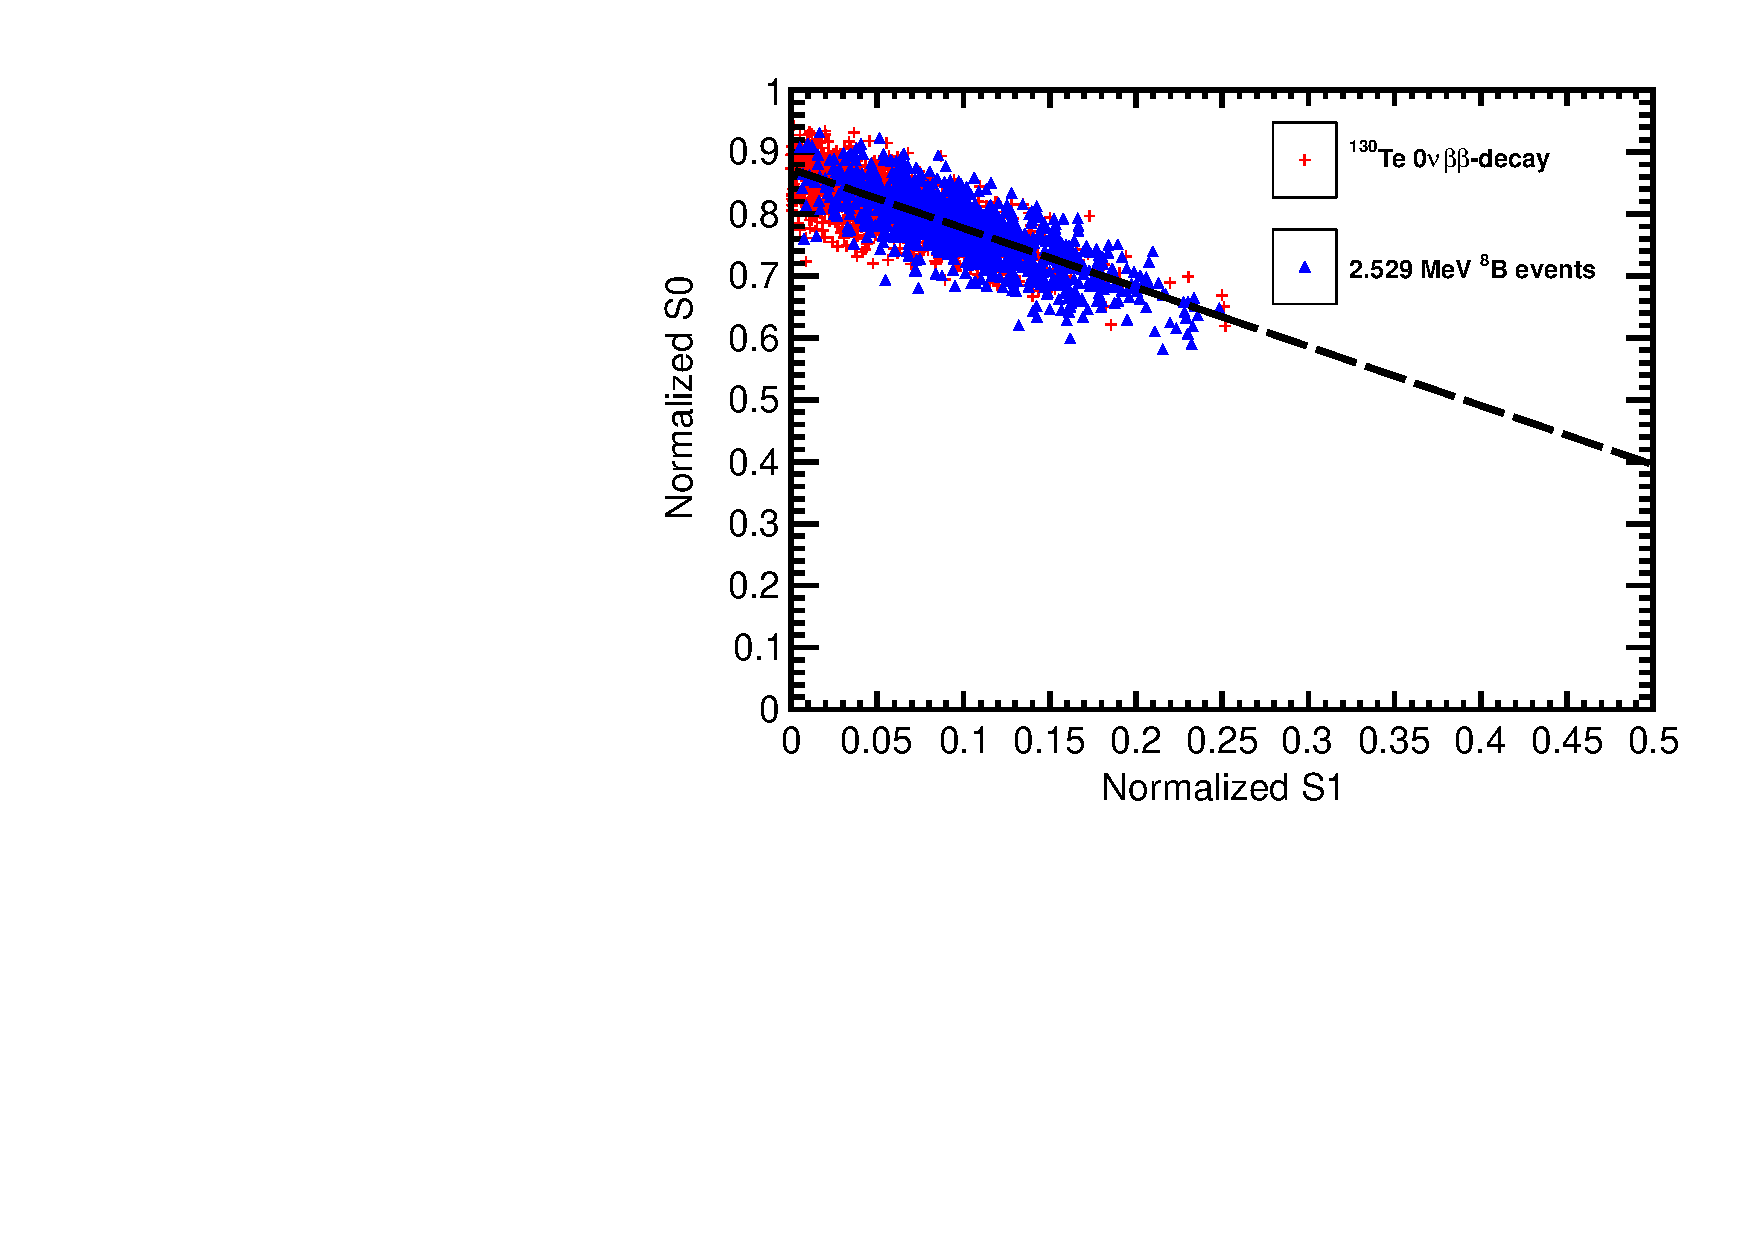
\includegraphics[angle=0,width=0.49\textwidth]{plots/hS0vsS1_Te130_1el_allLight_VtxSmear0cm_VtxShiftX0cm_momDT1p0ns_rndVtx_3p0mSphere.pdf}
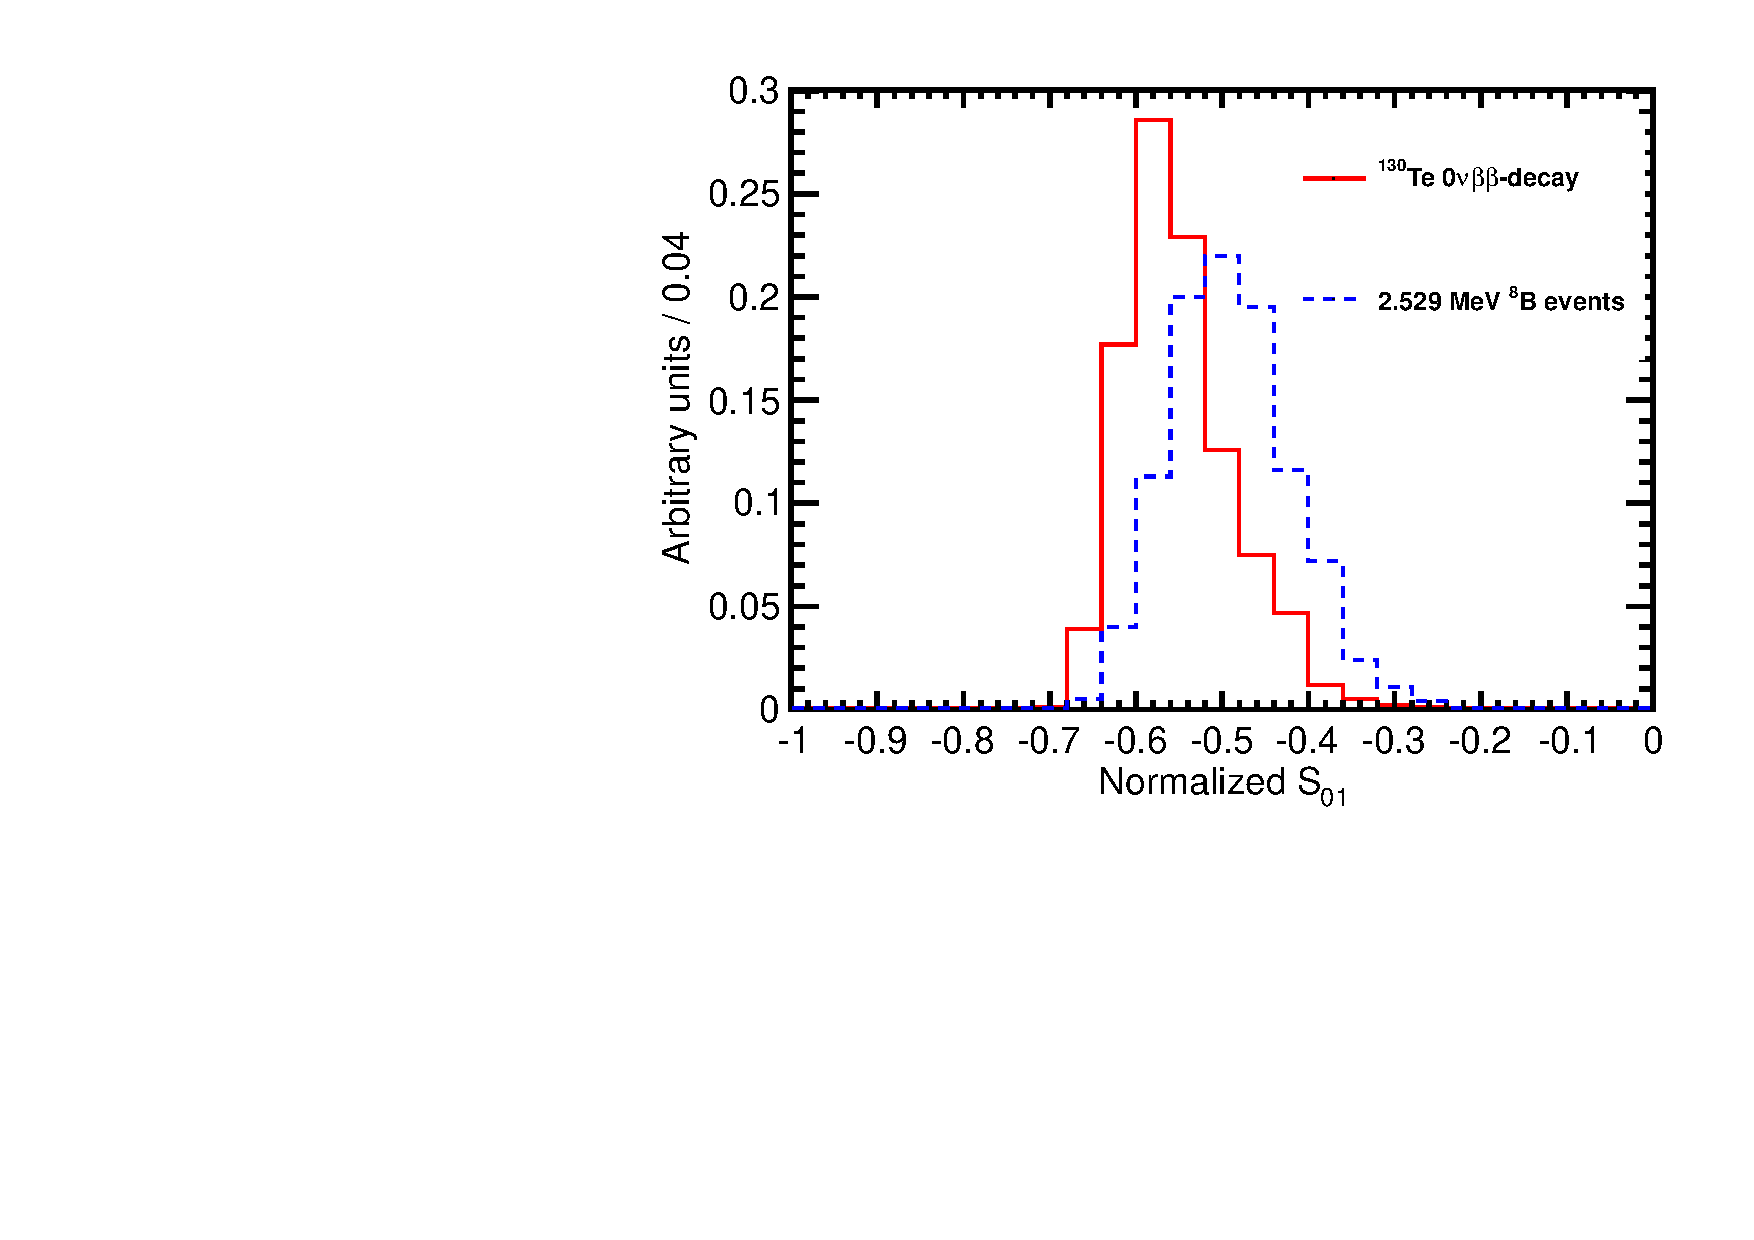
\includegraphics[angle=0,width=0.49\textwidth]{plots/hS01_allLight_VtxSmear0cm_VtxShiftX0cm_momDT1p0ns_rndVtx_3p0mSphere.pdf}
\caption{Spherical harmonics comparison between $\Te$ $\vbb$-decay signal (Q$=$2.529~MeV) (red) and $\B$ solar neutrinos background (blue) for 1000 simulated events.Verticies are uniformly distributed within the fiducial volume, R$<$3~m. $^8$Be events are implemented as 2.529~MeV electrons with the initial momentum direction uniformly distributed within 4$\pi$ solid angle. Perfect vertex reconstruction - true vertex position is used. (Left) S$_0$ versus S$_1$ scatter plot. Black dotted line is a linear fit of these 2D histograms. Variable S$_{01}$ is defined as a projection of 2D distribution onto this linear fit. (Right) S$_{01}$}
\label{fig:SL_Te_SmearX0cm_momDT1ns_rndVtx_3p0m}
\end{figure}



Imprecise knowledge of the vertex position due to finite resolution is another factor affecting performance of the spherical harmonics analysis. Small deviations in vertex reconstruction cause large effect on $S_0$ and $S_1$ for single electron event topology. For the verticies shifted along the direction of the electron the $\Delta t$ cut makes uniform scintillation light distribution less uniform. The $\Delta t$ cut selects more forward emitted photons in the case when the reconstructed vertex is shifted to the direction opposite to the electron momentum (enhancing forward region populated by Cherenkov photons - more asymmetric photon distribution causing higher values of $S_1$). It selects more backward emitted photons in the case when the reconstructed vertex is shifted in the direction along the electron momentum (counter balancing forward region populated by Cherenkov photons - more symmetric photon distribution causing smaller values of $S_1$).

\begin{figure}[htb]
\centering
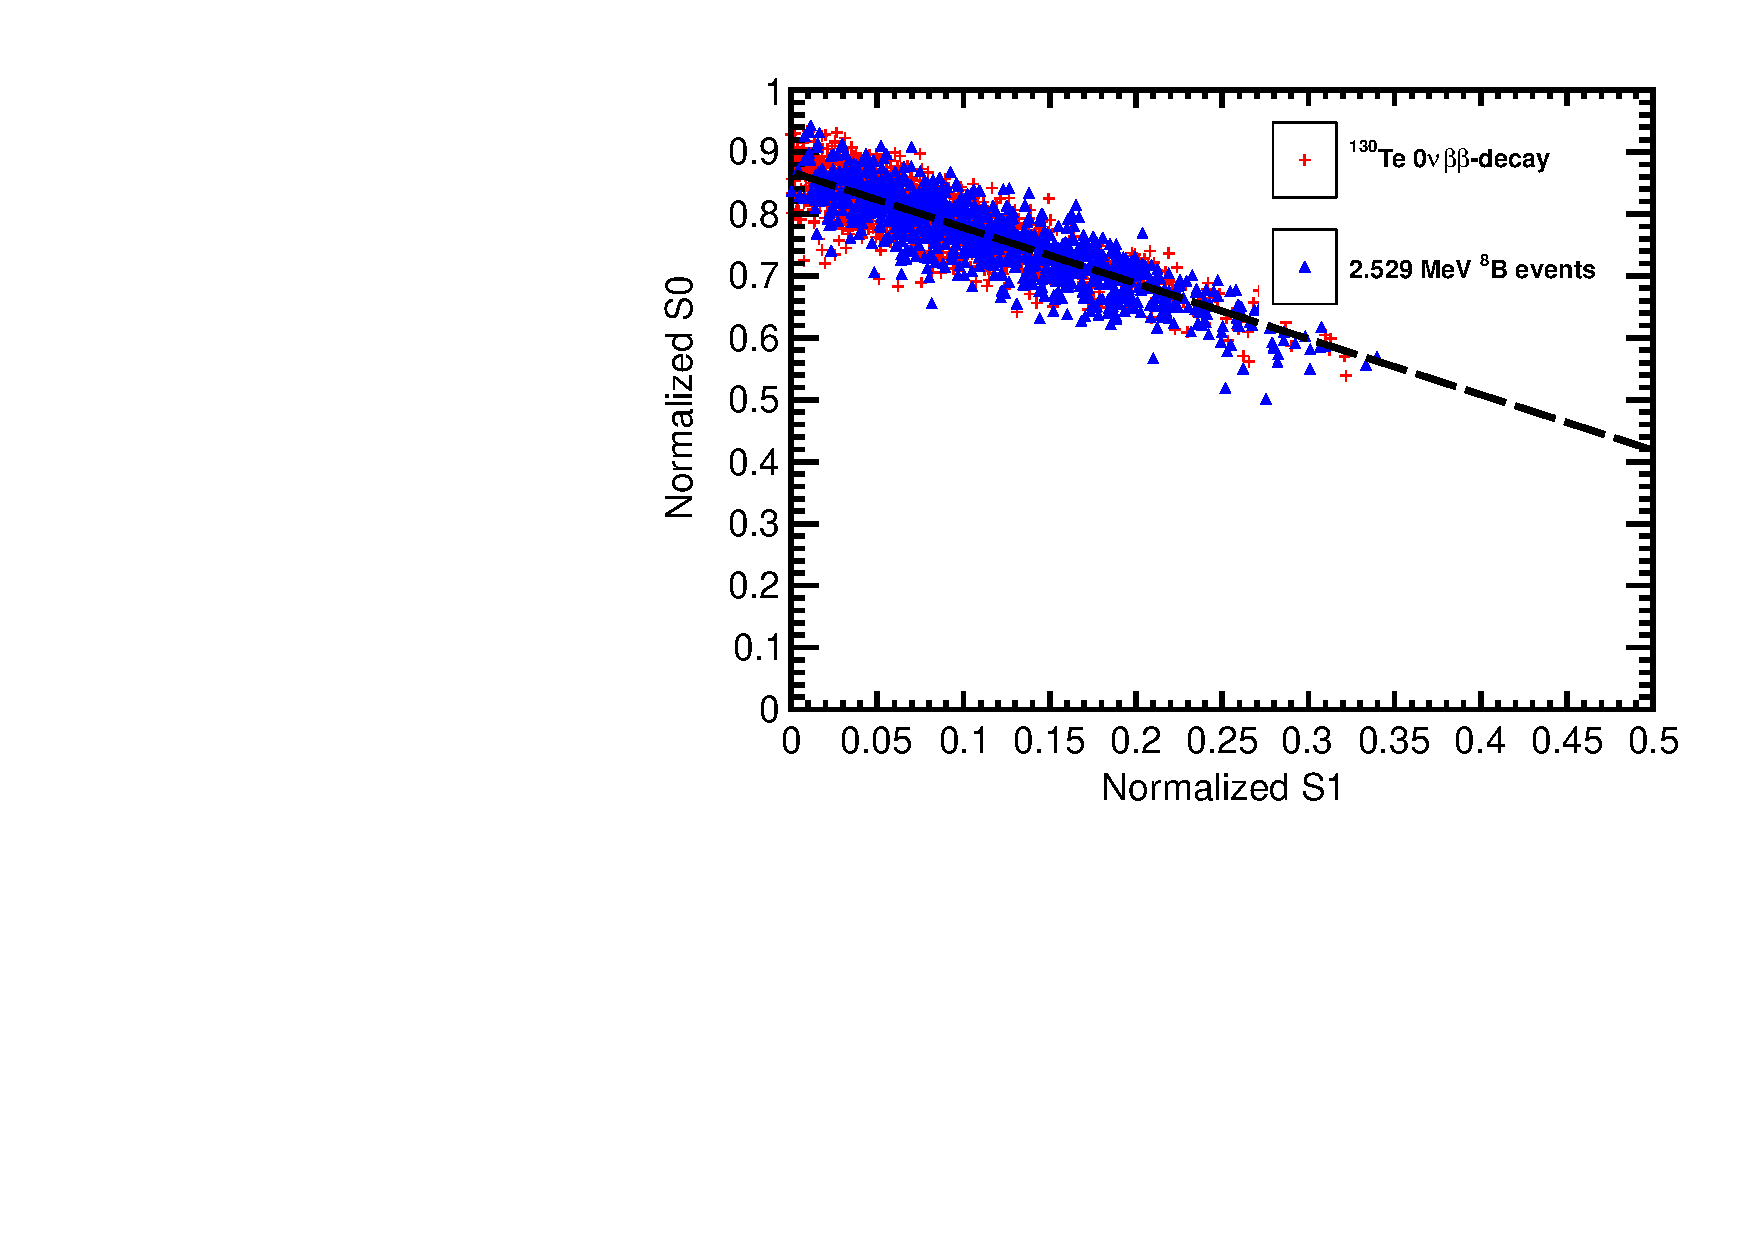
\includegraphics[angle=0,width=0.49\textwidth]{plots/hS0vsS1_Te130_1el_allLight_VtxSmear3cm_VtxShiftX0cm_momDT1p0ns_rndVtx_3p0mSphere.pdf}
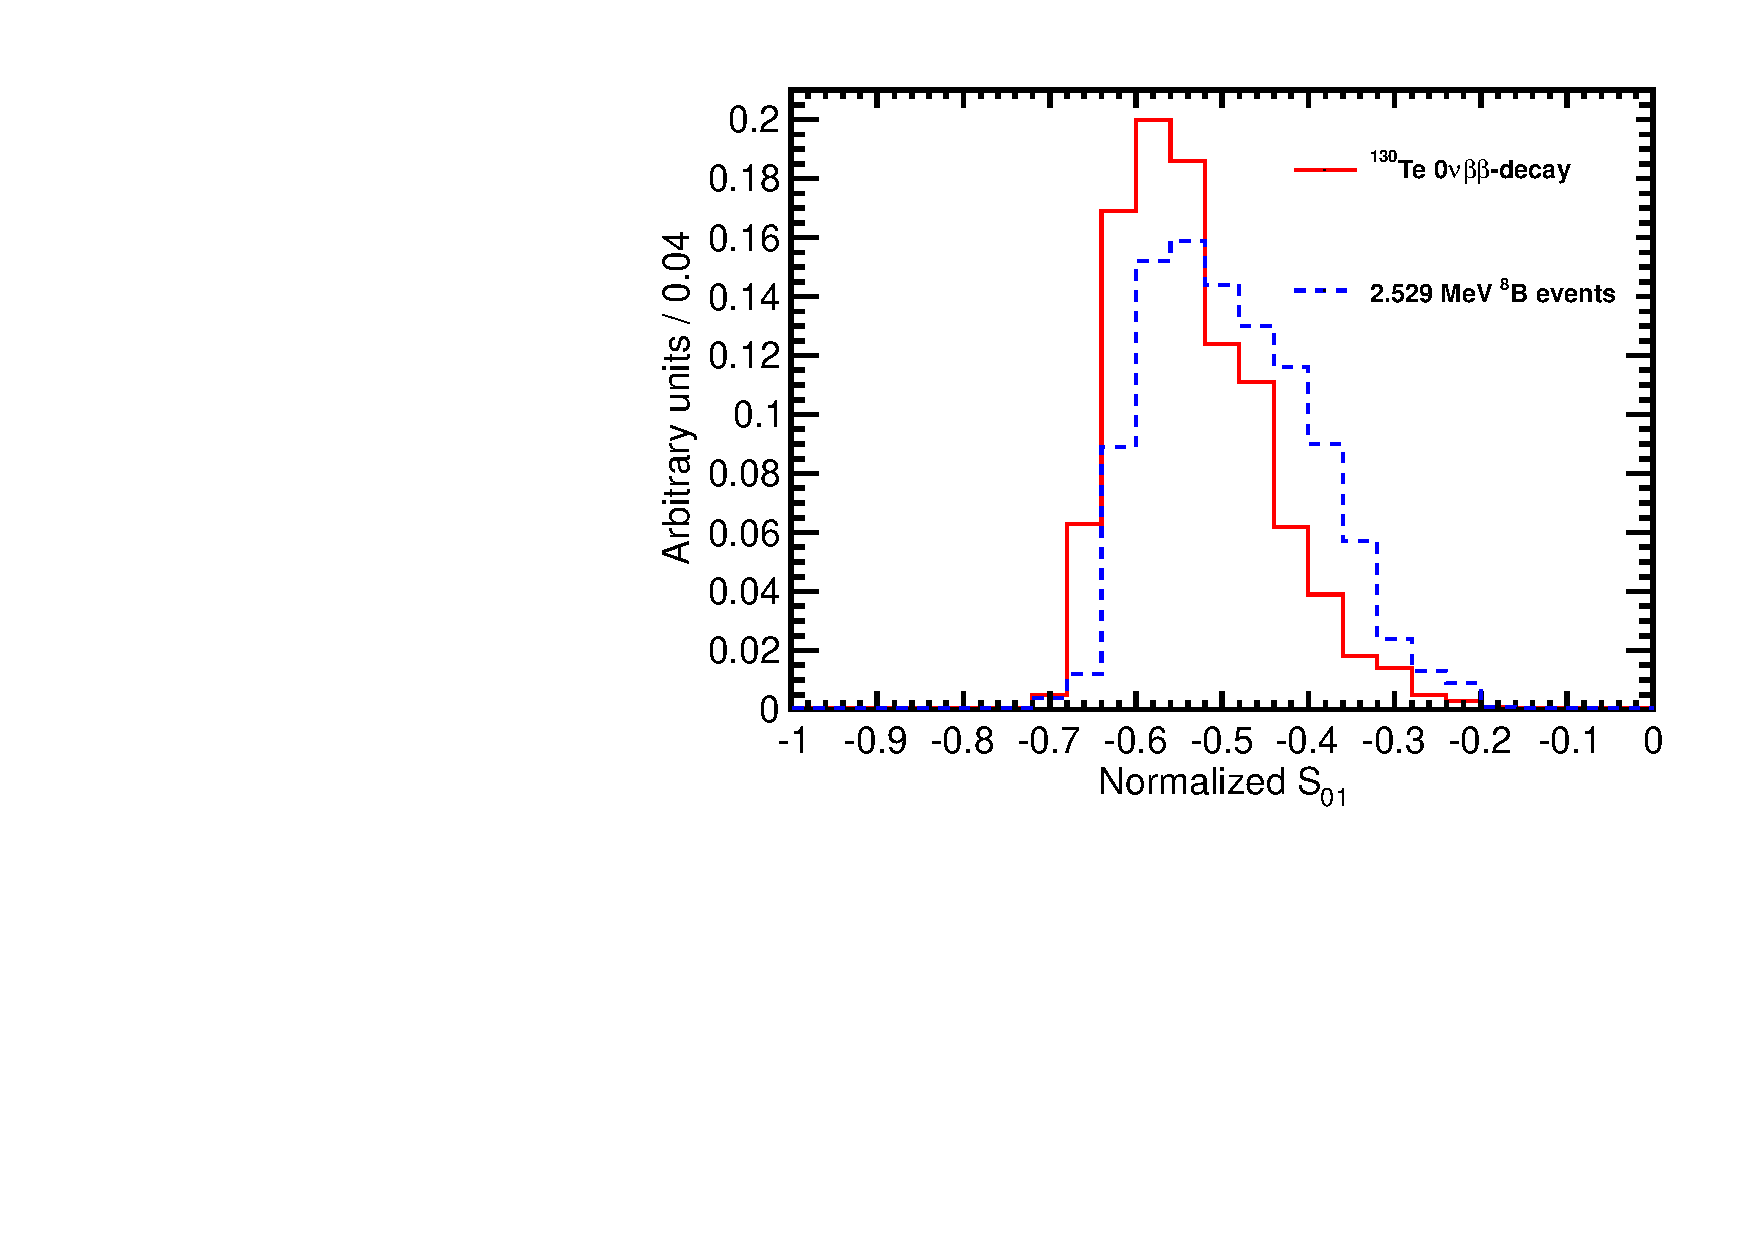
\includegraphics[angle=0,width=0.49\textwidth]{plots/hS01_allLight_VtxSmear3cm_VtxShiftX0cm_momDT1p0ns_rndVtx_3p0mSphere.pdf}
\caption{Spherical harmonics comparison between $\Te$ $\vbb$-decay signal (Q$=$2.529~MeV) (red) and $\B$ solar neutrinos background (blue) for 1000 simulated events.Verticies are uniformly distributed within the fiducial volume, R$<$3~m. $^8$Be events are implemented as 2.529~MeV electrons with the initial momentum direction uniformly distributed within 4$\pi$ solid angle. Vetrex is smeared with 3~cm resolution. (Left) S$_0$ versus S$_1$ scatter plot. Black dotted line is a linear fit of these 2D histograms. Variable S$_{01}$ is defined as a projection of 2D distribution onto this linear fit. (Right) S$_{01}$}
\label{fig:SL_Te_SmearX3cm_momDT1ns_rndVtx_3p0m}
\end{figure}


{\bf Solution to this problem would be a better selection criteria of early light. It has to preserve high admixture of the Cherenkov photons, but needs to select scintillation photons in a more uniform manner. Working on it, but may not be simple so I don't want to include it in this paper.}

Good vertex resolution is essential for spherical harmonics analysis. Such strong dependence on the vertex resolution can be addressed by choosing a different liquid scintillator mixture with a more delayed emission of the scintillation  light. Figure~\ref{fig:SL_Te_momDT1ns_sci0p5ns_rndVtx_3p0m} shows spherical harmonics calculated for the time profile which has scintillation component delayed by 0.5ns with respect to what is shown in Fig.~\ref{fig:Arrival_time}


\begin{figure}[htb]
\centering
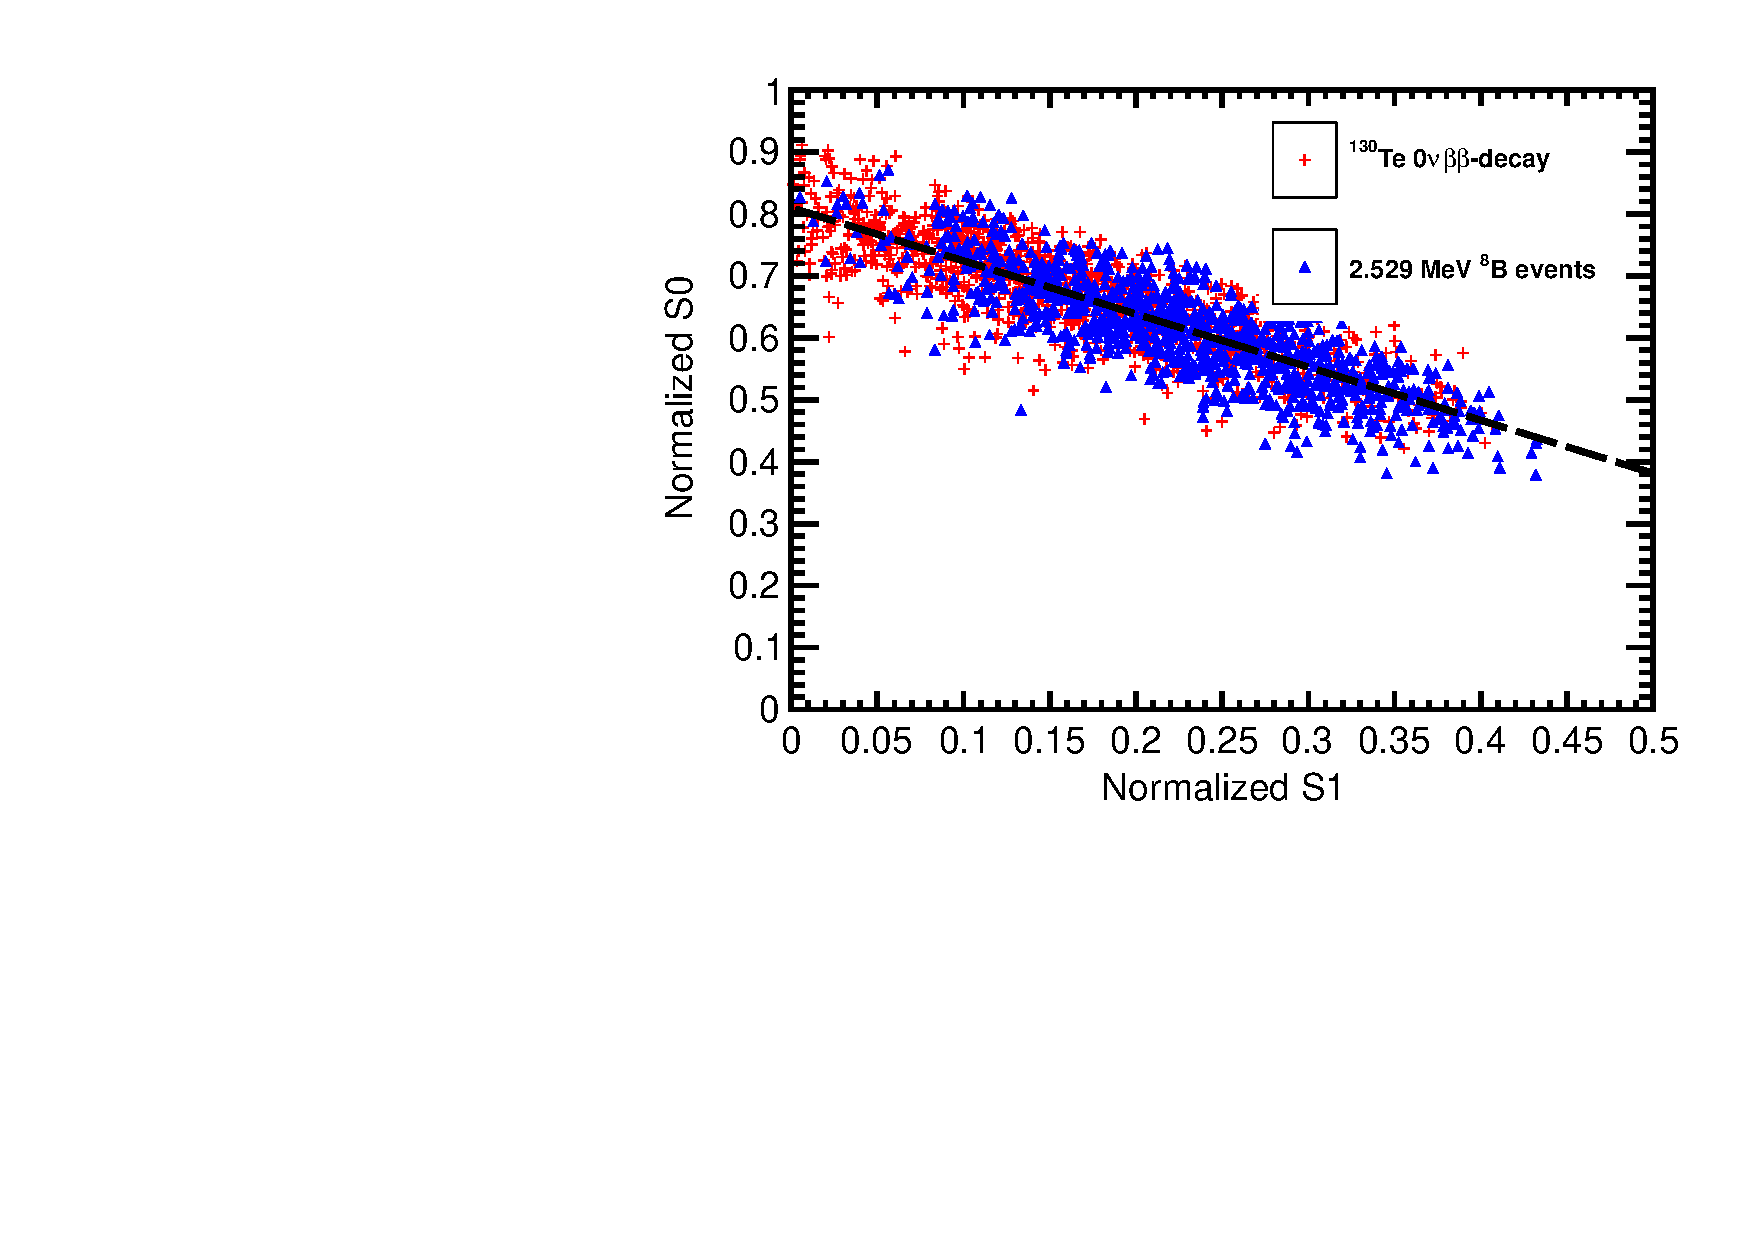
\includegraphics[angle=0,width=0.49\textwidth]{plots/hS0vsS1_Te130_1el_allLight_VtxSmear3cm_VtxShiftX0cm_momDT1p0ns_sci0p5ns_rndVtx_3p0mSphere.pdf}
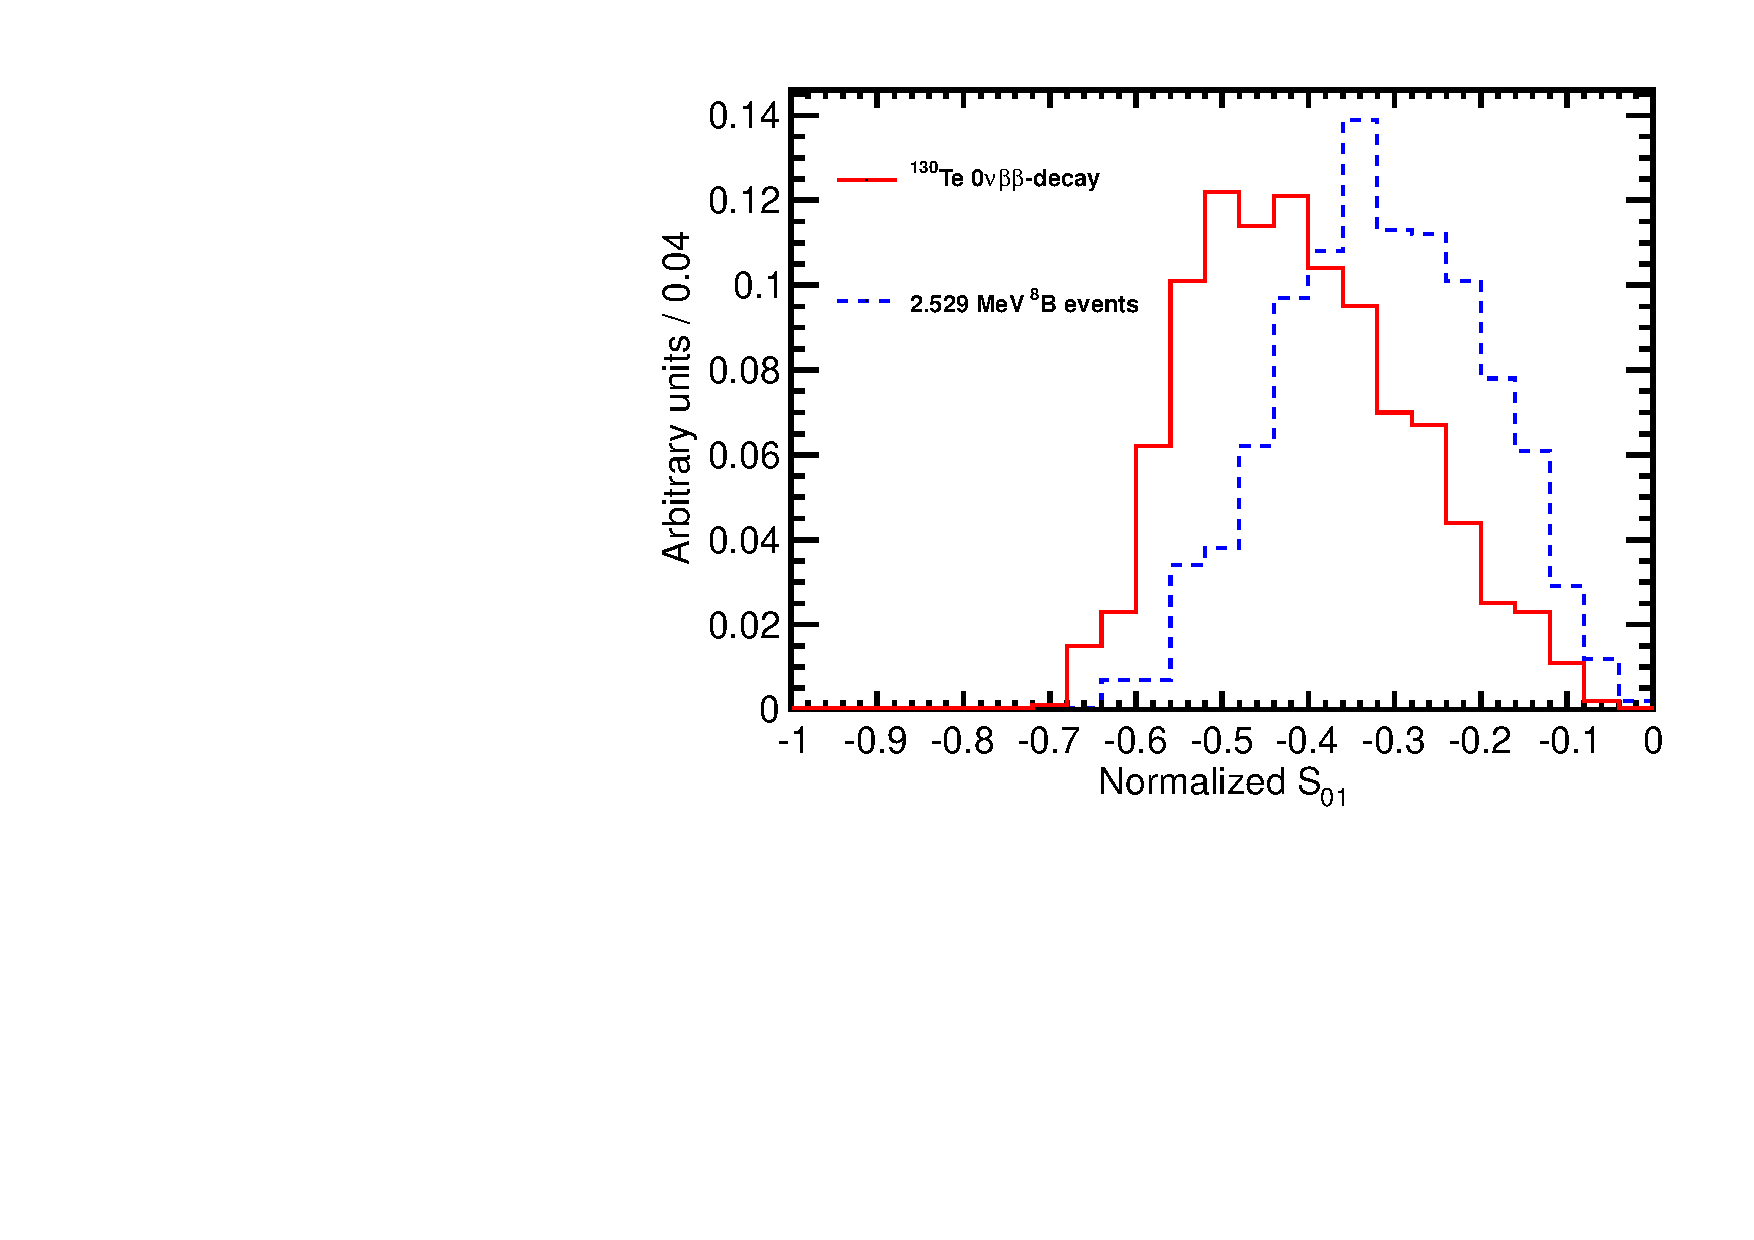
\includegraphics[angle=0,width=0.49\textwidth]{plots/hS01_allLight_VtxSmear3cm_VtxShiftX0cm_momDT1p0ns_sci0p5ns_rndVtx_3p0mSphere.pdf}
\caption{Spherical harmonics comparison between $\Te$ $\vbb$-decay signal (Q$=$2.529~MeV) (red) and $\B$ solar neutrinos background (blue) for 1000 simulated events.Verticies are uniformly distributed within the fiducial volume, R$<$3~m. $^8$Be events are implemented as 2.529~MeV electrons with the initial momentum direction uniformly distributed within 4$\pi$ solid angle. Vetrex is smeared with 3~cm resolution. {\bf Scintillation light is delayed by additional 0.5~ns.} (Left) S$_0$ versus S$_1$ scatter plot. Black dotted line is a linear fit of these 2D histograms. Variable S$_{01}$ is defined as a projection of 2D distribution onto this linear fit. (Right) S$_{01}$}
\label{fig:SL_Te_SmearX3cm_momDT1ns_sci0p5ns_rndVtx_3p0m}
\end{figure}


\section{Conclusions}
A technique based on spherical harmonics analysis is discussed to separate $\vbb$-decay from $\B$ solar neutrino interactions. The separation is based on distinct event topologies of signal and background. This event topology information is available in addition to the measurements of the energy deposited in the detector. This technique may be further developed and adopted by future large scale liquid scintillator detectors to suppress background coming from $\B$ solar neutrino interactions in the detector volume. The performance of the technique is mostly affected by chromatic dispersions, vertex reconstruction and time profile of the emission of the scintillation light. We show that a liquid scintillator detector with a $\sim$1~ns total delay of the scintillation light with respect to the Cherenkov light allows for use of spherical harmonics analysis as an extra handle to extract $\vbb$-decay signal.


\section{Acknowledgments}
To be finalized based on opt-in for the author list.
%We thank G.~Orebi-Gann for discussions on the backgrounds and sensitivity of the SNO+ experiment. We thankful to Evan Angelico for help with investigation of how various detector parameters affect vertex reconstruction. We thank Chandler Schlupf for help with sensitivity calculations. We thank Christopher Aberle, Brian Naranjo, Eric Spieglan and Matt Wetstein for fruitful discussions on event topology and vertex reconstruction. This work was done with support from DOE (grant number) and NSF (grant number).


\appendix

\section{$\vbb$-decay vs $^{10}$C background}

Other common backgrounds to $\vbb$-decay search include radioactive decays of nuclei excited by cosmic muons and decays of Th and U naturally present in the materials. In a liquid scintillator detectors most of events from Th and U decays are happening in the materials of the scintillator enclosure. Typically they enter the fiducial volume as 2.6~MeV gammas. These gammas either shower too late or have mis-reconstructed vertex. Both effects depend on details of a particular experiment and therefore in this paper we make no attempt to introduce a topology reconstruction for the backgrounds coming from Th and U lines. Cosmic induced backgrounds, to the contrary, are more generic and originate inside the fiducial volume. In this section we discuss event topology of $\Cten$ events that are most relevant in the energy of 2-3~MeV.

Typical energy deposition by $\Cten$ events is shown in Fig.~\ref{fig:Edep_C10}. We propose to use spherical harmonics analysis to separate $\vbb$-decay events from $\Cten$ events that within energy resolution overlap with the $\vbb$-decay Q-value.



\begin{figure}[htb]
\centering
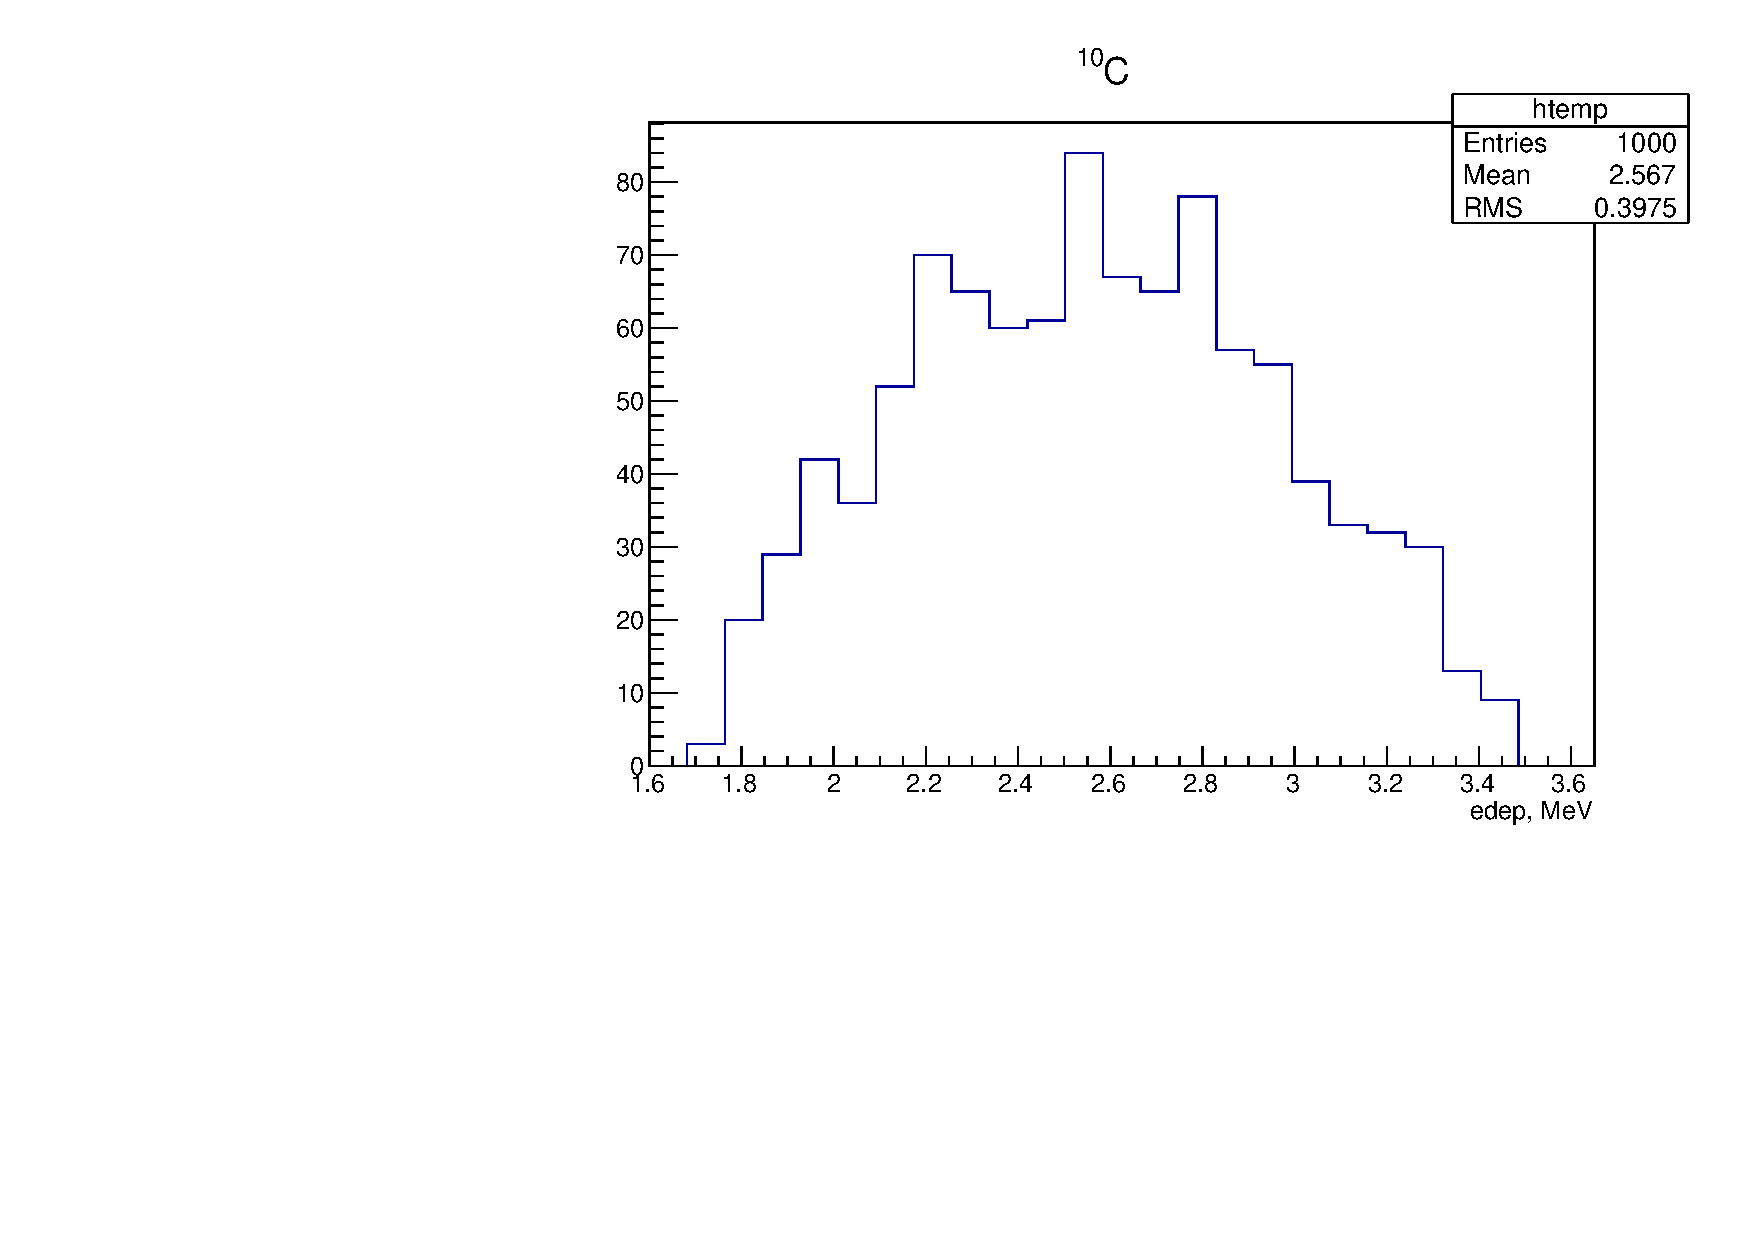
\includegraphics[angle=0,width=0.95\textwidth]{plots/hEdep_C10.pdf}
\caption{Energy deposition in $\Cten$ events.}
\label{fig:Edep_C10}
\end{figure}

\begin{figure}[htb]
\centering
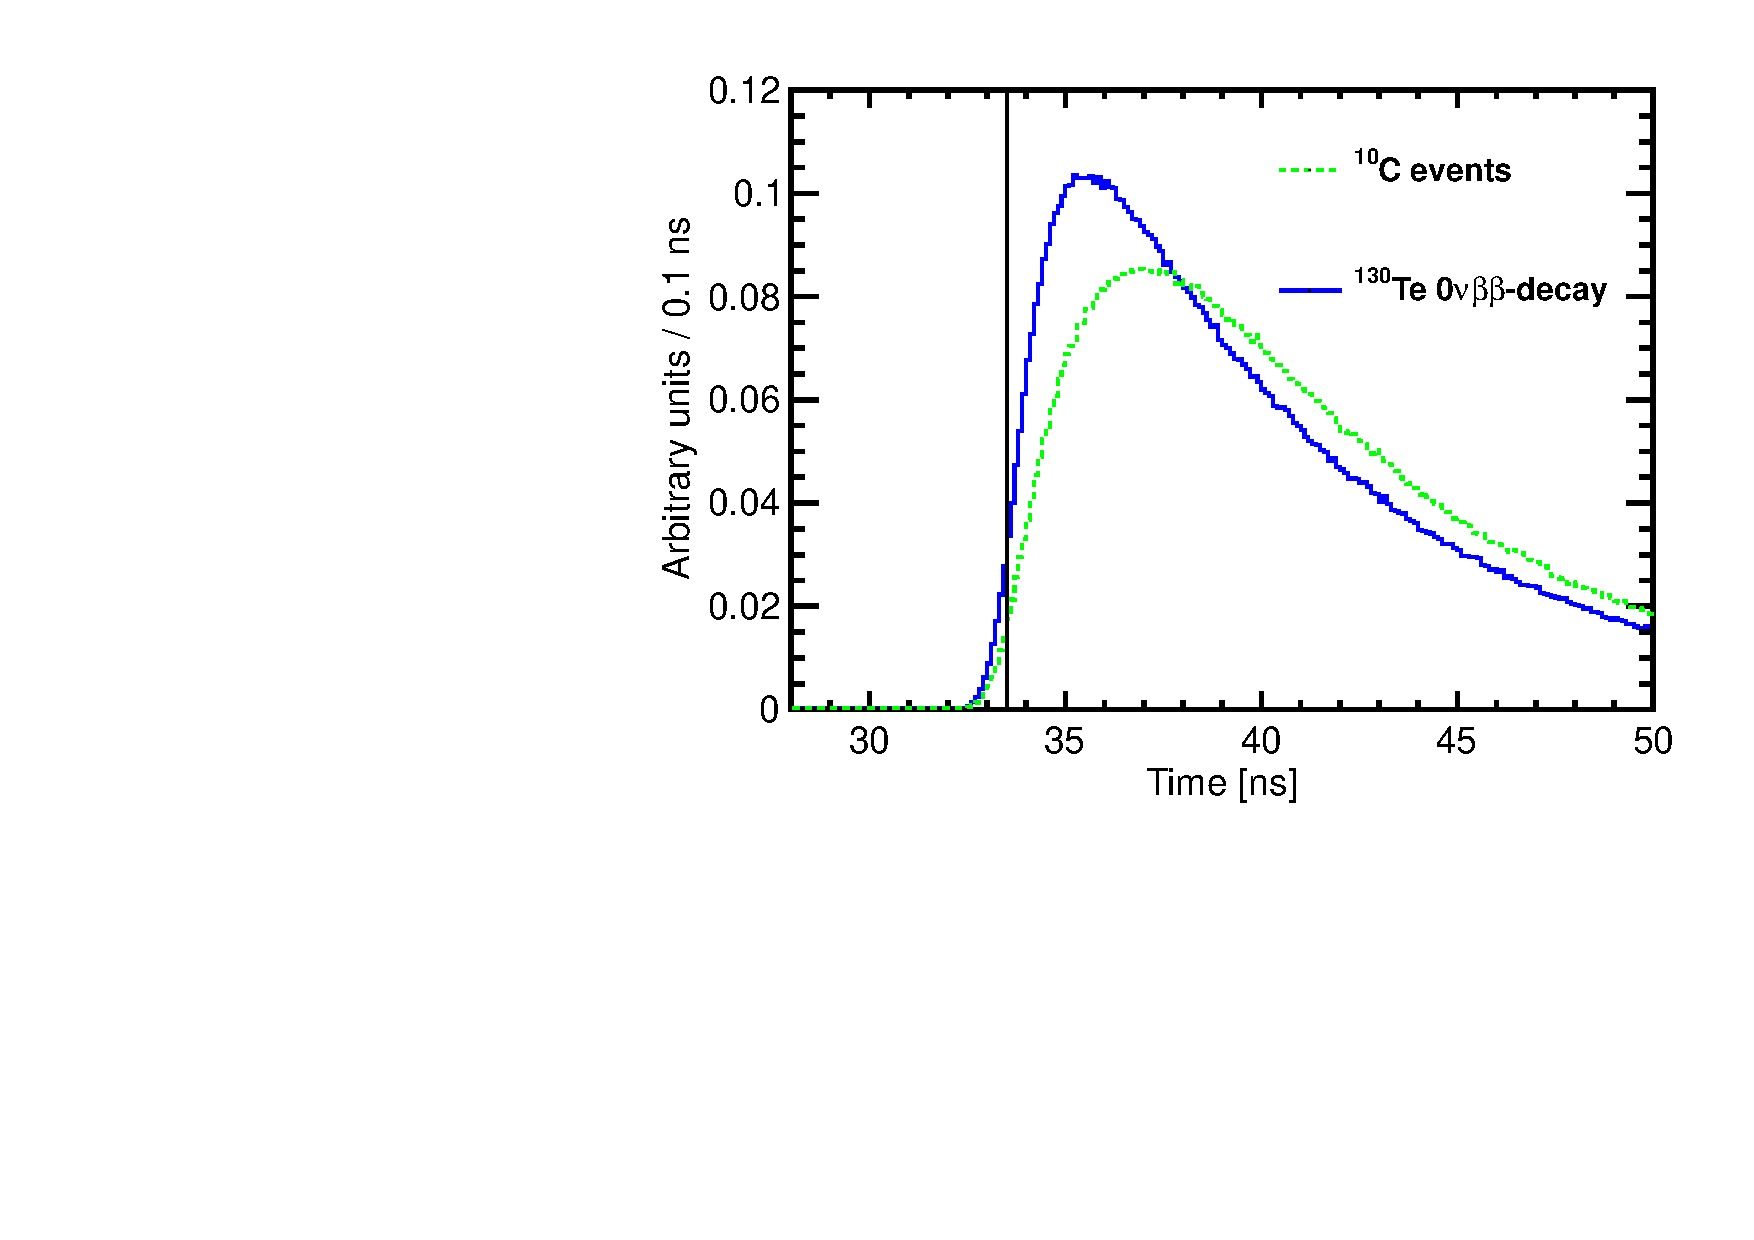
\includegraphics[angle=0,width=0.45\textwidth]{plots/hT_C10.pdf}
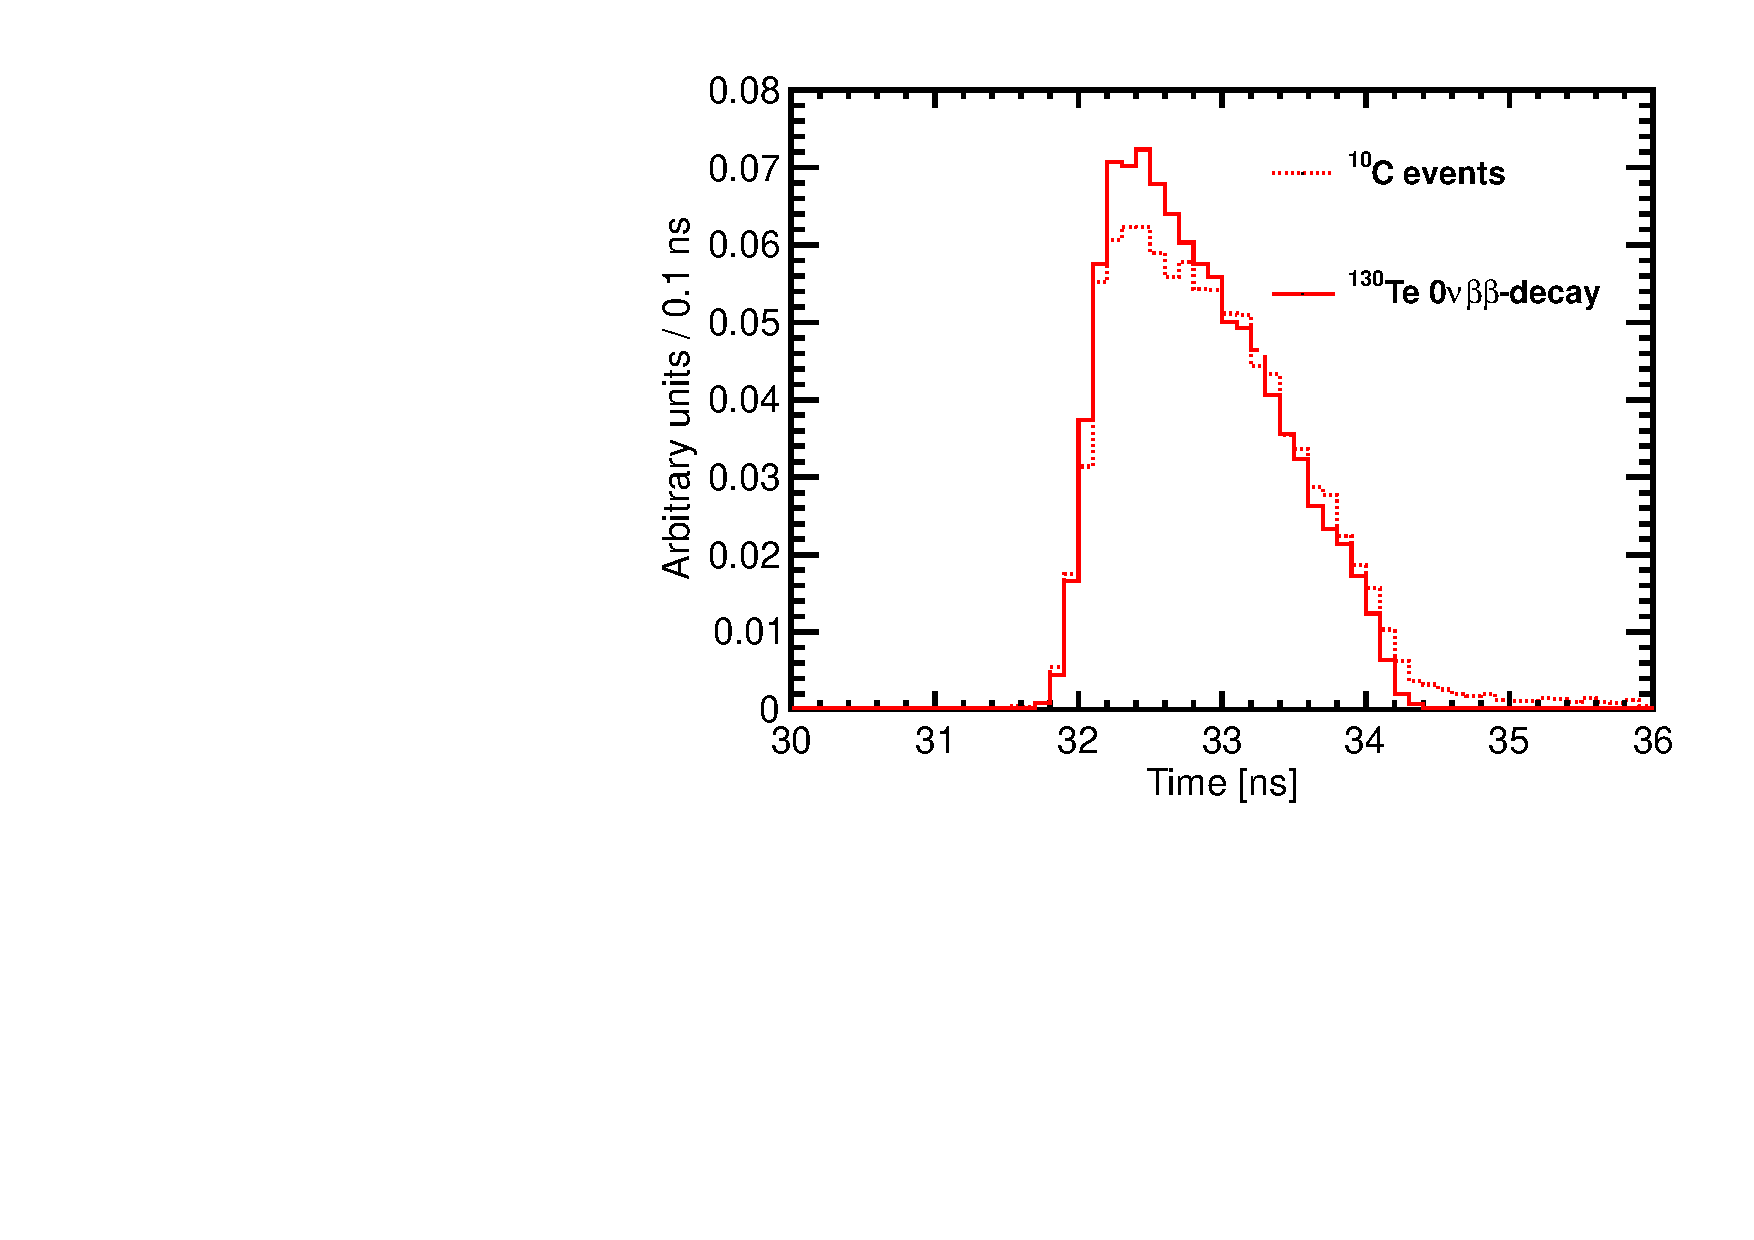
\includegraphics[angle=0,width=0.45\textwidth]{plots/hTche_C10.pdf}
\caption{Photo-electron (PE) arrival times after application of the photo-detector transit time spread (TTS) of 100~ps for the simulation of 1000 $\vbb$-decay events of $\Te$ (solid lines) and $\Cten$ (dotted lines) events at the center of the detector. All distributions are normalized for shape comparison. {\bf Absolute number of PEs per event depends on the total energy deposited in the detector. Figure~\ref{fig:Edep_C10} shows energy deposited in the detector in $\Cten$ events.} (Left) Scintillation PEs arrival time. The black vertical line illustrates a time cut at 33.5 ns. (Right) Cherenkov PEs arrival time.}
\label{fig:Arrival_time_C10}
\end{figure}

We note that 98\% of $\Cten$ decays through the excited state of $\Bten$(718) that has a half-life time of $\sim$1~ns. Therefore majority of $\Cten$ events have a prompt positron accompanied by a delayed 0.718~MeV gamma. This delayed gamma affects PEs arrival time distribution. Figure~\ref{fig:Arrival_time_C10} shows shape comparison of PEs arrival time distribution between $\Te$ $\vbb$-decay and  $\Cten$ events. Time profile of the scintillation photons can be used to separate signal from $\Cten$ events.


\begin{figure}[htb]
\centering
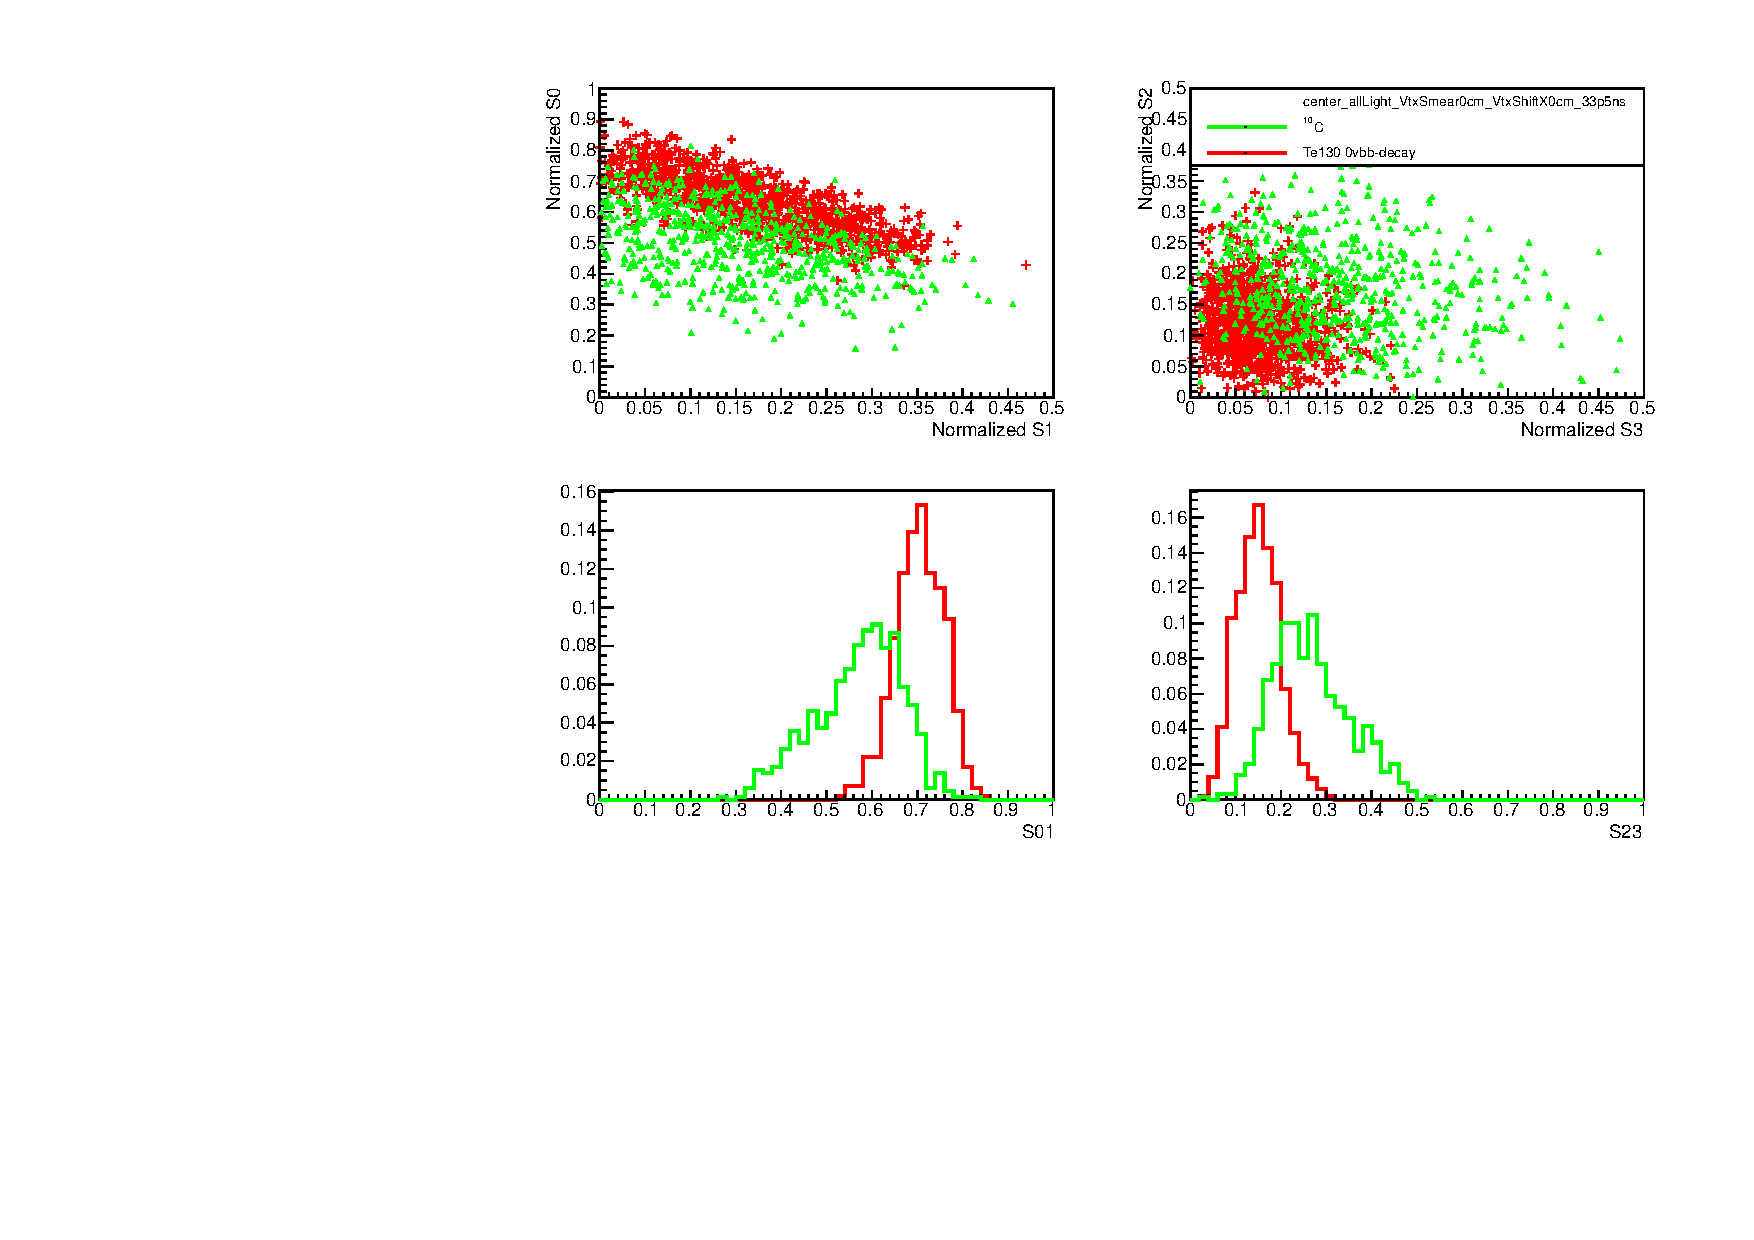
\includegraphics[angle=0,width=0.95\textwidth]{plots/hSLPlots_C10_allLight_VtxSmear0cm_VtxShiftX0cm_33p5ns_center.pdf}
\caption{Spherical harmonics comparison between $\Te$ $\vbb$-decay signal (Q$=$2.529~MeV) (red) and $\Cten$ solar neutrinos background (blue) for 1000 simulated events originated at the center of the sphere. $\Cten$ with energy deposition between 2.1~MeV and 2.9~MeV are considered. Perfect vertex reconstruction - true vertex position is used. Time cut of 33.5~ns on the photon arrival time is applied. (Top left) S$_0$ versus S$_1$ scatter plot. (Top right) S$_2$ versus S$_3$ scatter plot. (Bottom left) Distribution of the S$^{C10}_{01}$ variable calculated for signal (red) and background (green). (Bottom right) Distribution of the S$^{C10}_{23}$ variable calculated for signal (red) and background (green).}
\label{fig:SL_C10_33p5ns_center}
\end{figure}


Comparison of spherical harmonics is shown in Fig.~\ref{fig:SL_C10_33p5ns_center}. $\Cten$ events are generated at the center of the detector. True vertex position is used to apply a 33.5~ns time cut to select photons for the spherical harmonics analysis. The separation is seen in S0 vs S1 and S2 vs S3 scatter plots. We project both scatter plots to a line that gives maximum separation (two bottom panels in Fig.~\ref{fig:SL_C10_33p5ns_center}).

%\section{$\vbb$-decay vs backgrounds from Th and U series}

\begin{thebibliography}{00}
\bibitem{Directionality} C.~Aberle et al. JINST 9 P06012.
\bibitem{SNOp_paper} A good ref to SNO+ backgrounds description.
\end{thebibliography}

\end{document}
